%!TEX program = xelatex
\documentclass[fontset=fandol]{ctexart}
\setmainfont{Times New Roman}
\usepackage[a4paper,left=2.5cm,right=2.5cm,top=2cm,bottom=2cm]{geometry}
\usepackage{amsmath,amssymb,amsfonts,amsthm}
\usepackage{mathrsfs,bm,bbm}
\usepackage{fancyhdr}
\usepackage[colorlinks=true,linkcolor=black,citecolor=black,urlcolor=black]{hyperref}
\usepackage{enumitem}
\usepackage{booktabs,longtable,array,tabularx,multirow}
\usepackage{xparse,xstring}
\usepackage{lastpage}
\usepackage{color}
\usepackage{graphicx}
\usepackage{tikz}
\usetikzlibrary{arrows.meta,calc,angles,positioning,shapes.geometric,graphs}
\usepackage[framemethod=TikZ]{mdframed}

\lhead{\today}
\rhead{Page \thepage\ of \pageref{LastPage}}
\cfoot{}
\setlength{\headheight}{13pt}
\pagestyle{fancy}

\mdfdefinestyle{extrastyle}{%
    linecolor=gray,
    linewidth=0.8pt,
    frametitlerule=true,
    frametitlebackgroundcolor=gray!10,
    backgroundcolor=gray!5,
    skipabove=10pt,
    skipbelow=10pt,
    innertopmargin=6pt,
    innerbottommargin=6pt
}
\newenvironment{extra}{\begin{mdframed}[style=extrastyle, frametitle={* 选读内容（不要求掌握）}]}{\end{mdframed}}

\newcounter{DefinitionCounter}[section]
\newcounter{TheoremCounter}[section]
\newcounter{PropositionCounter}[section]
\newcounter{ExampleCounter}[section]
\newcounter{ExerciseCounter}[section]
\newcounter{ProblemCounter}[section]
\newcounter{ConclusionCounter}[section]
\NewDocumentEnvironment{definition}{O{}}
{\par\noindent\refstepcounter{DefinitionCounter}\textbf{定义\theDefinitionCounter\IfStrEq{#1}{}{}{ #1}}\quad}
{\par\vspace{0.8em}}
\NewDocumentEnvironment{theorem}{O{}}
{\par\noindent\refstepcounter{TheoremCounter}\textbf{定理\theTheoremCounter\IfStrEq{#1}{}{}{ #1}}\quad}
{\par\vspace{0.8em}}
\NewDocumentEnvironment{proposition}{O{}}
{\par\noindent\refstepcounter{PropositionCounter}\textbf{性质\thePropositionCounter\IfStrEq{#1}{}{}{ #1}}\quad}
{\par\vspace{0.8em}}
\NewDocumentEnvironment{example}{O{}}
{\par\noindent\refstepcounter{ExampleCounter}\textbf{例\theExampleCounter\IfStrEq{#1}{}{}{ #1}}\quad}
{\par\vspace{0.8em}}
\NewDocumentEnvironment{exercise}{O{}}
{\par\noindent\refstepcounter{ExerciseCounter}\textbf{练习\theExerciseCounter\IfStrEq{#1}{}{}{ #1}}\quad}
{\par\vspace{0.8em}}
\NewDocumentEnvironment{problem}{O{}}
{\par\noindent\refstepcounter{ProblemCounter}\textbf{问题\theProblemCounter\IfStrEq{#1}{}{}{ #1}}\quad}
{\par\vspace{0.8em}}
\NewDocumentEnvironment{conclusion}{O{}}
{\par\noindent\refstepcounter{ConclusionCounter}\textbf{结论\theConclusionCounter\IfStrEq{#1}{}{}{ #1}}\quad}
{\par\vspace{0.8em}}
\newenvironment{custom}[1]{\par\noindent\textbf{#1}\quad}{\par\vspace{0.8em}}
\newenvironment{proofdetail}{\par\noindent\textbf{证明}\quad}{\hfill$\square$\par\vspace{0.8em}}
\newenvironment{solution}{\par\noindent\textbf{解}\quad}{\hfill$\square$\par\vspace{0.8em}}
\newenvironment{idea}{\par\noindent\textbf{思路}\quad}{\par\vspace{0.4em}}
\newenvironment{warning}{\par\noindent\textbf{易错点}\quad}{\par\vspace{0.8em}}
\newcommand{\renewEnvironmentCounter}{\setcounter{DefinitionCounter}{0}\setcounter{TheoremCounter}{0}\setcounter{PropositionCounter}{0}\setcounter{ExampleCounter}{0}\setcounter{ExerciseCounter}{0}\setcounter{ProblemCounter}{0}\setcounter{ConclusionCounter}{0}}
\newcommand{\dd}{\mathrm{d}}
\newcommand{\ee}{\mathrm{e}}
\newcommand{\RR}{\mathbbm{R}}
\newcommand{\upcite}[1]{\textsuperscript{\textsuperscript{\cite{#1}}}}
\newcommand{\bec}{\kern 0.56em\bigcirc \kern -0.85em {\small \because}\kern 0.56em}
\DeclareMathOperator*{\argmax}{\mathrm{arg\,max}}
\DeclareMathOperator*{\argmin}{\mathrm{arg\,min}}
\renewcommand{\textfraction}{0.15}
\renewcommand{\topfraction}{0.85}
\renewcommand{\bottomfraction}{0.65}
\renewcommand{\floatpagefraction}{0.60}
\renewcommand{\figurename}{图}
\renewcommand{\tablename}{表}
\setlength{\belowcaptionskip}{4pt}
\setlength{\abovecaptionskip}{4pt}

\title{大学数学I讲义\\完整合并版}
\author{数学科学学院课程讲义草稿}
\date{\today}

\begin{document}
\maketitle
\vspace{-1em}

\renewcommand{\contentsname}{\hspace*{\fill}\Large\bfseries 目\quad 录 \hspace*{\fill}}
\setcounter{tocdepth}{2}
\tableofcontents
\clearpage

\section{数学文化与数学史导引}
\renewEnvironmentCounter

这一节供课下阅读. 它不要求大家记忆年代和人名，而希望帮助大家看到：数学并不是孤立公式的堆积，而是在长期解决问题的过程中形成的一套语言. 一个数学概念通常经历三步：先在实际问题中反复出现，再被抽象为稳定对象，最后被放入由定义、定理和证明组成的逻辑系统. 本讲义后面使用“定义--定理--证明--例题”的写法，正是为了让计算有根据，让应用有边界.

\subsection{河谷文明：从测量和记账到算法}

数学最初常常从实际需要中生长出来. 尼罗河泛滥后要重新丈量土地，粮食征收和工程建设需要稳定的计算规则，天文观测和历法编制需要处理周期. 因此，早期数学首先表现为算法：给出一套可重复执行的步骤，使不同的人在相同数据下得到相同结果.

古埃及纸草书中保存了分数、面积和体积计算的题目；美索不达米亚泥板中可以看到二次方程、倒数表和与勾股数组有关的材料. 这些内容的共同特征是重视“怎样算”. 例如计算一块田地面积时，真实田地可能边界不规则，数学处理会先把它近似成三角形、梯形或若干简单图形的组合，再用可操作的规则求面积. 这里已经有建模思想：现实对象先被简化为数学对象，然后才进入计算.

本课程开头学习数列，也可以从这种算法传统理解. 数列描述按步骤产生的量，例如人口逐期增长、药物多次给药后的浓度、贷款余额的递推变化. 极限则回答更深的问题：当步骤无限继续时，某个量是否趋于稳定？这个问题不能只靠观察前几项回答，所以需要 $\varepsilon$--$N$ 语言来规定“最终稳定”的精确含义.

\subsection{希腊数学：证明为什么成为数学的核心}

如果说早期算法回答“怎样算”，那么古希腊数学突出追问“为什么一定对”. 欧几里得的《几何原本》把几何知识组织成定义、公设、公理、命题和证明. 这种写法的意义在于：一旦承认起点和推理规则，后续结论就不再依赖画图是否准确，也不依赖某个例子是否看起来成立.\footnote{关于欧几里得的生平与《几何原本》的影响，可参见 MacTutor: \url{https://mathshistory.st-andrews.ac.uk/Biographies/Euclid/}.}

一个典型例子是 $\sqrt2$ 的无理性. 在边长为 $1$ 的正方形中，对角线长度满足 $d^2=2$. 若假设 $d=\frac pq$ 为既约分数，则
\[
p^2=2q^2.
\]
于是 $p^2$ 为偶数，故 $p$ 为偶数，设 $p=2k$. 代回得
\[
4k^2=2q^2,\qquad q^2=2k^2,
\]
所以 $q$ 也为偶数. 这与 $\frac pq$ 既约矛盾. 因此 $\sqrt2$ 不是有理数. 这个证明很短，却说明了一个深刻事实：数轴上仅有有理数并不够，几何长度会迫使我们扩充数系.

阿基米德在面积和体积问题中进一步发展了逼近思想. 他用内接和外切多边形估计圆周率，也用类似穷竭法的思想研究抛物线弓形面积、球的体积和表面积.\footnote{关于阿基米德及其穷竭法思想，可参见 MacTutor: \url{https://mathshistory.st-andrews.ac.uk/Biographies/Archimedes/}.} 这些工作虽然还没有现代极限符号，却已经非常接近本课程中的核心观念：用一列越来越精细的近似对象夹住目标量，并证明误差可以任意小.

阿波罗尼奥斯系统研究圆锥曲线，给出了椭圆、抛物线、双曲线等对象的几何理论.\footnote{关于阿波罗尼奥斯和圆锥曲线，可参见 MacTutor: \url{https://mathshistory.st-andrews.ac.uk/Biographies/Apollonius/}.} 后来解析几何把这些曲线写成方程，微积分又研究这些曲线的切线、面积和极值. 从几何图形到代数方程，再到导数和积分，这是数学语言逐层精密化的过程.

\subsection{中国古代数学：问题集、算法与逼近}

中国古代数学很重视“问题--算法--校验”的传统. 《九章算术》以问题集方式组织材料，内容涉及面积体积、比例分配、工程计算、线性方程组和勾股问题. 例如“方程”章用算筹排列未知量系数，本质上是在处理线性方程组；这种列阵计算与今天线性代数中的消元法有明显联系.\footnote{关于中国数学传统，可参见 MacTutor 的 Chinese mathematics overview: \url{https://mathshistory.st-andrews.ac.uk/HistTopics/Chinese_overview/}.}

刘徽为《九章算术》作注时，不满足于只给算法，而是说明算法成立的理由. 他的割圆术是极限思想的一个重要历史实例：用圆内接正多边形的面积逼近圆面积，边数越多，多边形越接近圆. 若用现代语言表达，就是构造一列近似值，并研究它们是否趋向一个确定的量. 这与后来用数列极限定义圆周率、面积和积分有共同精神.

祖冲之父子在圆周率计算上给出了很精确的结果；孙子算经中有后来被称为“中国剩余定理”的同余问题；秦九韶在《数书九章》中给出多项式求值方法，现代常称为秦九韶算法. 这些例子说明，中国数学并不只是“算术技巧”，其中包含算法复杂度、误差控制和结构化计算的雏形. 对今天学习数学的学生来说，这一传统很有启发：严谨证明保证结论可靠，算法实现保证方法可以落地.

\subsection{变化的语言：微积分}

微积分的形成，是因为人们需要同时处理两类问题：一类是瞬时变化，例如速度、切线斜率、边际成本；另一类是累积总量，例如面积、路程、总收益. 费马研究曲线切线和极值，笛卡尔把几何问题转化为代数方程，牛顿从运动和力学出发发展“流数法”，莱布尼茨则形成了影响深远的微分符号 $\dd x,\dd y$ 和积分符号 $\int$.\footnote{关于微积分兴起的历史脉络，可参见 MacTutor: The rise of calculus, \url{https://mathshistory.st-andrews.ac.uk/HistTopics/The_rise_of_calculus/}.}

以切线问题为例，割线斜率为
\[
\frac{f(x+\Delta x)-f(x)}{\Delta x}.
\]
当 $\Delta x$ 趋于 $0$ 时，如果这个比值趋于确定数，就得到切线斜率，也就是导数. 以面积问题为例，把曲边图形切成许多窄条并求和，窄条越细，总和越接近真实面积. 这两类问题表面上一个求局部变化，一个求整体累积，但微积分基本定理揭示了它们之间的内在联系.

本讲义后半部分的导数、中值定理和 Taylor 公式都属于这条主线. 导数把“局部变化”变成极限；中值定理说明局部变化率与整体变化之间存在严格联系；Taylor 公式则告诉我们，在适当条件下，复杂函数可以用多项式近似. 这些内容在经济学中的边际分析、管理学中的优化问题、医学中的剂量反应模型、机器学习中的损失函数最小化中都会反复出现.

\subsection{严谨化：从直觉无穷小到极限语言}

早期微积分大量使用“无穷小量”的直觉，这使计算非常有效，但也带来逻辑困难：无穷小既像不是零，又常常在计算中被忽略. 十九世纪以后，柯西、魏尔斯特拉斯等人用极限语言重建微积分基础. 今天我们说
\[
\lim_{x\to x_0}f(x)=A,
\]
不是说 $x$ 真的“到达” $x_0$，而是说只要允许误差足够小，就能找到相应的邻域，使函数值落入指定误差范围. 这正是 $\varepsilon$--$\delta$ 或 $\varepsilon$--$N$ 语言的作用.

因此，严格性并不是把简单问题变复杂，而是在处理“无限逼近”“瞬时变化”“无穷求和”时避免误判. 例如从前几项看起来趋近某数，并不能证明数列收敛；图像看起来有切线，也不能替代导数存在的验证；通项趋于零，也不能保证级数收敛. 这些都是本课程反复强调定义和定理条件的原因.

\subsection{从计算机到人工智能}

二十世纪以来，数学与计算机科学相互推动. 算法需要离散数学、极限估计和误差控制；数据建模需要概率统计、线性代数和优化理论；人工智能中的许多训练过程，本质上是在高维参数空间中寻找使损失函数变小的方向.\footnote{关于人工智能的概念与历史背景，可参见 Stanford Encyclopedia of Philosophy, Artificial Intelligence: \url{https://plato.stanford.edu/entries/artificial-intelligence/}.}

例如梯度下降法的基本形式为
\[
\theta_{k+1}=\theta_k-\eta\nabla L(\theta_k),
\]
其中 $L$ 是损失函数，$\nabla L$ 是梯度，$\eta$ 是学习率. 这个公式背后正是导数的含义：导数或偏导数描述函数沿某个方向变化的快慢，负梯度方向通常给出局部下降最快的方向. 在线性回归中，损失函数常取
\[
L(w,b)=\frac1m\sum_{i=1}^m(wx_i+b-y_i)^2.
\]
训练模型就是调节 $w,b$，使预测值 $wx_i+b$ 尽量接近观测值 $y_i$. 求导告诉我们 $w,b$ 应向哪个方向改动；凸性则帮助判断是否会陷入局部极小. 因此，学习导数不是只为了画切线，也是在学习现代优化算法的基础语言.

\subsection{一条贯穿本课程的线索}

可以把本课程看成三次递进. 第一，极限把“无限过程”纳入严格讨论：数列是否稳定，函数是否趋近某值，级数是否收敛. 第二，连续与导数把“变化”变成可计算对象：函数图像是否断裂，瞬时变化率是否存在，局部信息能否推出整体结论. 第三，微分和 Taylor 公式把“近似”变成有控制的工具：在误差可估计的前提下，用简单表达式代替复杂表达式.

斐波那契数列可以作为一个小例子贯穿这三层. 它由递推关系
\[
a_{n+2}=a_{n+1}+a_n
\]
给出，体现“按步骤生成”的思想；相邻两项比值若收敛，则极限 $r$ 满足
\[
r=1+\frac1r,
\]
从而得到黄金分割数
\[
r=\frac{1+\sqrt5}{2}.
\]
这里既有递推，也有极限，还有从具体数列抽象出稳定比例的过程.\footnote{关于 Fibonacci 数列和黄金分割的基本事实，可参见 Wolfram MathWorld, Fibonacci Number: \url{https://mathworld.wolfram.com/FibonacciNumber.html}.}

\section{数列的基本概念}

\subsection{从高中数列说起}

在高中数学中，我们已经接触过两种重要的数列。

\begin{example}[等差数列]
若数列 $\{a_n\}$ 满足
\[
a_{n+1}-a_n=d\qquad(n=1,2,\ldots),
\]
其中 $d$ 为常数，则称 $\{a_n\}$ 为等差数列，$d$ 称为公差. 由递推式逐项相加可得
\[
a_n=a_1+(n-1)d.
\]
例如 $1,3,5,7,\ldots$ 是公差为 $2$ 的等差数列.

等差数列前 $n$ 项和为
\[
S_n=\frac{n(a_1+a_n)}{2}.
\]
证明如下：将
\[
S_n=a_1+a_2+\cdots+a_n
\]
与倒序求和式
\[
S_n=a_n+a_{n-1}+\cdots+a_1
\]
相加，得到
\[
2S_n=(a_1+a_n)+(a_2+a_{n-1})+\cdots+(a_n+a_1).
\]
每一组括号内均为 $a_1+a_n$，共有 $n$ 组，故 $2S_n=n(a_1+a_n)$.
\end{example}

\begin{example}[等比数列]
若 $a_1\ne0$，且数列 $\{a_n\}$ 满足
\[
a_{n+1}=ra_n\qquad(n=1,2,\ldots),
\]
其中 $r$ 为常数，则称 $\{a_n\}$ 为等比数列，$r$ 称为公比. 由递推式可得
\[
a_n=a_1r^{\,n-1}.
\]
若 $r\ne1$，其前 $n$ 项和为
\[
S_n=a_1\frac{1-r^n}{1-r}.
\]
证明如下：由
\[
S_n=a_1+a_1r+\cdots+a_1r^{n-1}
\]
两边同乘 $r$，得
\[
rS_n=a_1r+a_1r^2+\cdots+a_1r^n.
\]
两式相减，得到 $(1-r)S_n=a_1(1-r^n)$，故上式成立. 当 $r=1$ 时，$S_n=na_1$.
\end{example}

\subsection{数列的一般定义}

从高中阶段的等差数列、等比数列出发，我们现在给出更一般也更精确的定义.

\begin{definition}[数列]
数列是定义在正整数集 $\mathbb{N}^+=\{1,2,3,\cdots\}$ 上、取实数值的函数. 若这个函数在 $n$ 处的函数值记为 $a_n$，则数列记为
\[
\{a_n\}:a_1,a_2,\ldots,a_n,\ldots .
\]
其中 $a_n$ 称为数列的第 $n$ 项或通项.
\end{definition}

这个定义说明，数列既有函数的本质，又有离散变量的特点. 函数 $y=f(x)$ 的自变量可以在区间中连续取值，而数列只在 $n=1,2,\ldots$ 这些正整数处取值. 因此，数列可以看作一种特殊函数：
\[
a_n=f(n),\qquad n\in\mathbb{N}^+.
\]
讨论数列时，项的顺序不可随意改变；同一组数字若排列顺序不同，通常就是不同数列.

\begin{example}
判断下列对象能否确定一个数列，并说明理由.
\[
(1)\ a_n=\frac{n+1}{2n-1};\qquad
(2)\ a_1=1,\ a_{n+1}=2a_n+1;\qquad
(3)\ 1,2,4,\ldots .
\]
\end{example}
\begin{custom}{解}
(1) 给出了通项公式，对每个正整数 $n$ 都能唯一确定 $a_n$，因此确定一个数列.

(2) 给出了初值和递推关系. 由 $a_1=1$ 可依次得到
\[
a_2=3,\quad a_3=7,\quad a_4=15,\ldots
\]
因此也确定一个数列.

(3) 只列出前三项，不能唯一确定一个数列. 例如 $a_n=2^{n-1}$ 的前三项为 $1,2,4$；但 $b_1=1,b_2=2,b_3=4,b_n=0(n\ge4)$ 也有同样前三项. 因此仅凭有限项通常不能严格确定无穷数列.
\end{custom}

\begin{example}
设某药物每隔固定时间给药一次，每次给药后体内新增浓度 $C_0$，两次给药之间保留比例为 $q$，其中 $0<q<1$. 若 $A_n$ 表示第 $n$ 次给药后体内药物浓度，则可建立递推模型
\[
A_{n+1}=qA_n+C_0.
\]
求该模型的稳定浓度.
\end{example}
\begin{custom}{解}
若 $A_n$ 收敛到稳定浓度 $A$，则在极限状态下应满足
\[
A=qA+C_0.
\]
解得
\[
A=\frac{C_0}{1-q}.
\]
为了说明这一步不是形式猜测，令 $B_n=A_n-A$. 由 $A=qA+C_0$ 及 $A_{n+1}=qA_n+C_0$ 得
\[
B_{n+1}=A_{n+1}-A=q(A_n-A)=qB_n.
\]
因此
\[
B_n=q^{n-1}B_1.
\]
由于 $0<q<1$，有 $q^{n-1}\to0$，所以 $B_n\to0$，即
\[
A_n\to A=\frac{C_0}{1-q}.
\]
\end{custom}

\subsection{数列的几种其他定义方式}

\begin{custom}{方式一：列出前几项}
例如：\(1, \dfrac12, \dfrac13, \dfrac14, \dots\)，猜想通项为 \(a_n = \dfrac1n\)。

注意：这种定义方式不严格，因为前几项可能对应多种通项。例如 \(1,2,4,\dots\) 可以是 \(a_n=2^{n-1}\)，也可以是 \(a_n = \dfrac{n^2-n+2}{2}\)。
\end{custom}

\begin{custom}{方式二：通项公式}
直接给出 \(a_n = \dfrac{n+1}{2n-1}\)，则可算出任意一项。这是最常用的定义方式。
\end{custom}

\begin{custom}{方式三：递推关系}
用前面项表示后面项。例如：
\[
a_1 = 1,\ a_2 = 1,\ a_n = a_{n-1} + a_{n-2}\ (n \geq 3),
\]
这就是著名的\textbf{斐波那契数列}：\(1,1,2,3,5,8,13,21,\dots\)

自然界中很多现象与斐波那契数列有关：向日葵的种子排列（常出现 34,55,89 等斐波那契数）、鹦鹉螺的螺旋线、甚至兔子繁殖问题。
\end{custom}

\subsection{数列在生活与生产中的应用}

数列不仅仅是课本上的抽象概念，它在我们的日常生活和现代生产中有着广泛的应用。下面介绍几个有趣的实例。

\begin{custom}{应用一：算法分析与计算机科学}

在计算机科学中，算法的\textbf{时间复杂度}经常用数列来描述。例如，考虑一个在有序数组中查找元素的算法：

\begin{itemize}
\item \textbf{二分查找}：每次将搜索范围缩小一半。在最坏情况下，需要查找的次数满足递推关系：
\[
T(n) = T\left(\dfrac{n}{2}\right) + 1,\quad T(1) = 1.
\]
解这个递推，得到 \(T(n) = \lceil \log_2 n \rceil\)。这是一个对数增长数列——非常高效！


一个著名的例子是\textbf{汉诺塔}问题：把 \(n\) 个圆盘从一根柱子移到另一根，最少需要移动的次数满足：
\[
H_n = 2H_{n-1} + 1,\quad H_1 = 1.
\]
解这个递推得 \(H_n = 2^n - 1\)——指数增长！64 个圆盘需要移动 \(2^{64}-1\) 次，即使每秒移动一次，也需要约 5849 亿年。
\end{itemize}
\end{custom}

\begin{custom}{应用二：自然界中的斐波那契数列}

斐波那契数列 \(1, 1, 2, 3, 5, 8, 13, 21, 34, 55, \ldots\) 在自然界中随处可见：

\begin{itemize}
\item \textbf{向日葵的花盘}：种子排列成两组螺旋线，一组顺时针，一组逆时针，数量通常是相邻的斐波那契数（如 34 和 55，或 55 和 89）。
\item \textbf{松果的鳞片}：排列也呈现斐波那契螺旋。
\item \textbf{鹦鹉螺的壳}：其对数螺线的生长比例接近黄金分割比 \(\varphi \approx 1.618\)，而 \(\varphi\) 与斐波那契数列密切相关（\(\lim_{n\to\infty} \dfrac{F_{n+1}}{F_n} = \varphi\)）。
\item \textbf{蜜蜂的家族树}：雄蜂（由未受精卵发育而来）的祖先数量构成斐波那契数列。
\item \textbf{花瓣数}：许多花的花瓣数是 3（百合）、5（飞燕草）、8（翠雀）、13（金盏花）、21（紫菀）等斐波那契数。
\end{itemize}

\begin{center}
\begin{tikzpicture}
% 简单的向日葵螺旋示意图
\foreach \i in {1,...,50} {
    \pgfmathsetmacro{\r}{0.3*sqrt(\i)}
    \pgfmathsetmacro{\theta}{137.5*\i}
    \filldraw[orange] (\theta:\r) circle (1.5pt);
}
\node at (0, -3) {向日葵种子的螺旋排列（示意图）};
\end{tikzpicture}
\end{center}

大自然为什么“偏爱”斐波那契数？科学家认为，这种排列方式可以让种子最紧密地堆积，充分利用空间——这是自然选择的结果，也是数学与生命的美妙交汇。
\end{custom}

\begin{custom}{应用三：工程中的递归设计与分形}

在工程和建筑设计领域，许多结构采用\textbf{自相似}的设计——即整体与局部形状相似。这种递归结构可以用数列来描述。

\begin{itemize}
\item \textbf{分形天线}：手机天线采用分形设计，可以在有限空间内获得更长的有效长度，从而接收更多频段的信号。
\item \textbf{谢尔宾斯基三角形}：一个不断“挖空”的三角形图案，它的面积随迭代次数构成一个等比数列：\(A_n = \left(\dfrac{3}{4}\right)^n A_0\)。
\item \textbf{科赫雪花}：一条不断“加尖”的曲线，它的周长随迭代次数无限增长（\(L_n = \left(\dfrac{4}{3}\right)^n L_0\)），但面积却收敛到有限值。
\end{itemize}

这些例子展示了：数列不仅是描述离散过程的工具，还连接着几何、物理和工程。
\end{custom}

\subsection{差分及其应用}

在微积分中，我们通过导数研究函数的变化率。对于数列，差分扮演着类似的角色。

\begin{definition}[差分]
对于数列 \(\{a_n\}\)，定义：
\begin{itemize}
\item 一阶差分：\(\Delta a_n = a_{n+1} - a_n\)；
\item 二阶差分：\(\Delta^2 a_n = \Delta(\Delta a_n) = a_{n+2} - 2a_{n+1} + a_n\)；
\item \(k\) 阶差分：\(\Delta^k a_n = \Delta(\Delta^{k-1} a_n)\)。
\end{itemize}
\end{definition}

\begin{proposition}[差分的性质]
\begin{enumerate}
\item \(\Delta C = 0\)（\(C\) 为常数）；
\item \(\Delta(C a_n) = C \Delta a_n\)；
\item \(\Delta(a_n + b_n) = \Delta a_n + \Delta b_n\)。
\end{enumerate}
\end{proposition}

差分的一个核心应用是数列求和。

\begin{theorem}[离散牛顿-莱布尼茨公式]
\[
\sum_{k=m}^{n-1} \Delta a_k = a_n - a_m.
\]
特别地，\(\sum_{k=1}^{n-1} \Delta a_k = a_n - a_1\)。
\end{theorem}

这个公式告诉我们：如果能找到一个数列 \(b_k\) 使得 \(\Delta b_k = a_k\)，那么 \(\sum a_k = b_n - b_1\)。这正是“差分是求和的逆运算”。

\begin{example}[求自然数平方和]
求 \(\sum_{k=1}^n k^2\)。
\end{example}

\begin{custom}{解}
观察发现 \(\Delta k^3 = (k+1)^3 - k^3 = 3k^2 + 3k + 1\)，所以
\[
3\sum_{k=1}^n k^2 = \sum_{k=1}^n \Delta k^3 - 3\sum_{k=1}^n k - \sum_{k=1}^n 1.
\]
利用 \(\sum k = \dfrac{n(n+1)}{2}\) 和 \(\sum 1 = n\)，以及 \(\sum \Delta k^3 = (n+1)^3 - 1\)，可得
\[
3\sum k^2 = (n+1)^3 - 1 - \dfrac{3n(n+1)}{2} - n = \dfrac{n(n+1)(2n+1)}{2},
\]
所以 \(\sum_{k=1}^n k^2 = \dfrac{n(n+1)(2n+1)}{6}\)。
\end{custom}

\begin{example}[进阶：求 \(\sum_{k=1}^n k^2 \cdot 2^k\)]
这类“多项式乘指数”的求和，可以用待定系数法构造差分。
\end{example}

\begin{custom}{解}
设 \(b_k = (Ak^2 + Bk + C)2^k\)，目标是使 \(\Delta b_k = k^2 2^k\)。
计算 \(\Delta b_k = b_{k+1} - b_k = [A(k+1)^2 + B(k+1) + C]2^{k+1} - (Ak^2 + Bk + C)2^k = 2^k[2A(k+1)^2 + 2B(k+1) + 2C - (Ak^2 + Bk + C)]\)。
整理得 \(\Delta b_k = 2^k[Ak^2 + (4A + B)k + (2A + 2B + C)]\)。
令其等于 \(k^2 2^k\)，比较系数：
\[
\begin{cases}
A = 1,\\
4A + B = 0,\\
2A + 2B + C = 0.
\end{cases}
\]
解得 \(A=1,\ B=-4,\ C=6\)，即 \(b_k = (k^2 - 4k + 6)2^k\)。
于是
\[
\sum_{k=1}^n k^2 2^k = \sum_{k=1}^n \Delta b_k = b_{n+1} - b_1 = [(n+1)^2 - 4(n+1) + 6]2^{n+1} - (1-4+6)\cdot 2 = (n^2 - 2n + 3)2^{n+1} - 6.
\]
\end{custom}

\subsection*{练习题：数列的定义、递推关系与差分}
\addcontentsline{toc}{subsection}{练习题：数列的定义、递推关系与差分}

\begin{exercise}写出下列数列的通项公式 \(a_n\)（用 \(n\) 表示）：
\begin{enumerate}
\item \(1, 3, 5, 7, 9, \dots\)
\item \(2, 4, 8, 16, 32, \dots\)
\item \(\dfrac{1}{2}, \dfrac{2}{3}, \dfrac{3}{4}, \dfrac{4}{5}, \dfrac{5}{6}, \dots\)
\item \(1, -\dfrac{1}{2}, \dfrac{1}{3}, -\dfrac{1}{4}, \dfrac{1}{5}, \dots\)
\end{enumerate}
\end{exercise}

\begin{exercise}已知下列递推关系及初始条件，写出数列的前 5 项：
\begin{enumerate}
\item \(a_1 = 3\)，\(a_n = 2a_{n-1}\)（\(n \geq 2\)）
\item \(a_1 = 1\)，\(a_n = a_{n-1} + n\)（\(n \geq 2\)）
\item \(a_1 = 1\)，\(a_2 = 3\)，\(a_n = a_{n-1} - a_{n-2}\)（\(n \geq 3\)）
\end{enumerate}
\end{exercise}

\begin{exercise}对于数列 \(a_n = n^2\)，计算：
\begin{enumerate}
\item 一阶差分 \(\Delta a_n\)
\item 二阶差分 \(\Delta^2 a_n\)
\item 三阶差分 \(\Delta^3 a_n\)
\end{enumerate}
观察结果，你能发现什么规律？
\end{exercise}

\begin{exercise}求下列递推数列的通项公式：
\begin{enumerate}
\item \(a_1 = 1\)，\(a_n = a_{n-1} + 3\)（\(n \geq 2\)）
\item \(a_1 = 5\)，\(a_n = a_{n-1} + 2n - 1\)（\(n \geq 2\)）
\item \(a_1 = 2\)，\(a_n = 2a_{n-1} + 1\)（\(n \geq 2\)）\quad（提示：可设 \(b_n = a_n + 1\) 构造等比数列）
\end{enumerate}
\end{exercise}

\begin{exercise}求一个数列 \(b_n\)，使得 \(\Delta b_n = n \cdot 2^n\)。
提示：设 \(b_n = (An + B)2^n\)，代入确定系数 \(A, B\)。
\end{exercise}

\begin{exercise}用差分法求下列和式：
\begin{enumerate}
\item \(\sum_{k=1}^{n} k\)
\item \(\sum_{k=1}^{n} k(k+1)\)
\end{enumerate}
\end{exercise}

\begin{exercise}已知斐波那契数列：\(F_1 = 1, F_2 = 1, F_n = F_{n-1} + F_{n-2} (n \geq 3)\)。
\begin{enumerate}
\item 计算比值 \(\dfrac{F_6}{F_5}, \dfrac{F_7}{F_6}, \dfrac{F_8}{F_7}, \dfrac{F_9}{F_8}, \dfrac{F_{10}}{F_9}\)，观察它们趋近于哪个数。
\item 证明：\(F_{n+1}F_{n-1} - F_n^2 = (-1)^n\)（卡西尼恒等式）。（选做）
\end{enumerate}
\end{exercise}

\begin{exercise}已知数列 \(\{a_n\}\) 满足 \(a_1 = 1\)，且对任意 \(n \geq 1\) 有 \(\Delta a_n = 3^n\)。
\begin{enumerate}
\item 求 \(a_n\) 的通项公式。
\item 计算 \(\sum_{k=1}^{n} k \cdot 3^{k-1}\)。（提示：利用 \(a_n\) 的表达式）
\end{enumerate}
\end{exercise}

\begin{exercise}已知一个数列的前几项为：\(a_1 = 1, a_2 = 5, a_3 = 14, a_4 = 30, a_5 = 55\)。
\begin{enumerate}
\item 计算该数列的一阶、二阶、三阶差分。
\item 根据差分结果判断 \(a_n\) 可能是几次多项式。
\item 求出 \(a_n\) 的通项公式。
\end{enumerate}
\end{exercise}

\begin{exercise}[较难：递推与差分的综合应用]
设数列 \(\{a_n\}\) 满足 \(a_1 = 1\)，且 \(a_{n+1} = 3a_n + 2^n\)（\(n \geq 1\)）。
\begin{enumerate}
\item 令 \(b_n = \dfrac{a_n}{2^n}\)，写出 \(b_n\) 满足的递推关系。
\item 求 \(b_n\) 的通项公式。
\item 求 \(a_n\) 的通项公式。
\item 计算 \(\sum_{k=1}^{n} a_k\)。
\end{enumerate}
\end{exercise}

\newpage 

\subsection*{参考答案提要}
\addcontentsline{toc}{subsection}{参考答案提要}
\begin{custom}{参考答案提要}

\begin{enumerate}
\item[(1)] (a) \(a_n = 2n-1\)；(b) \(a_n = 2^n\)；(c) \(a_n = \dfrac{n}{n+1}\)；(d) \(a_n = (-1)^{n-1} \dfrac{1}{n}\)。
\item[(2)] (a) \(3, 6, 12, 24, 48\)；(b) \(1, 3, 6, 10, 15\)；(c) \(1, 3, 2, -1, -3\)。
\item[(3)] \(\Delta a_n = 2n+1\)，\(\Delta^2 a_n = 2\)，\(\Delta^3 a_n = 0\)；规律：\(n^2\) 的二阶差分为常数，三阶及更高阶为 0。
\item[(4)] (a) \(a_n = 3n-2\)；(b) \(a_n = n^2 + 4\)；(c) \(a_n = 2^{n+1} - 1\)。
\item[(5)] \(b_n = (n-2)2^{n-1} + C\)（\(C\) 为任意常数）。
\item[(6)] (a) \(\dfrac{n(n+1)}{2}\)；(b) \(\dfrac{n(n+1)(n+2)}{3}\)。
\item[(7)] 比值趋近于 \(\dfrac{1+\sqrt{5}}{2} \approx 1.618\)。
\item[(8)] (a) \(a_n = \dfrac{3^n - 1}{2}\)；(b) \(\sum_{k=1}^{n} k \cdot 3^{k-1} = \dfrac{(2n-1)3^n + 1}{4}\)。
\item[(9)] 三阶差分为常数 3，是三次多项式，\(a_n = \dfrac{n^3 + 5n}{6}\)。
\item[(10)] (a) \(b_{n+1} = \dfrac{3}{2} b_n + \dfrac{1}{2}\)；(b) \(b_n = 3\left(\dfrac{3}{2}\right)^{n-1} - 1\)；(c) \(a_n = 3^n - 2^n\)；(d) \(\sum_{k=1}^{n} a_k = \dfrac{3^{n+1} - 3}{2} - (2^{n+1} - 2)\)。
\end{enumerate}
\end{custom}

\clearpage
\section{数列极限}

\subsection{从实数的完备性说起}

\textbf{一个历史故事：} 古希腊的毕达哥拉斯学派信奉“万物皆数”，认为一切量都可以表示为整数的比（即有理数）。然而，该学派成员希帕索斯发现，边长为 1 的正方形的对角线长度 \(\sqrt{2}\) 不能表示为两个整数的比。这个发现震惊了整个学派，这一发现说明，仅使用有理数无法完整刻画几何长度。

这个例子告诉我们：有理数是不够用的。数轴上还需要无理数来填补“空隙”。

\subsection{实数的构造与完备性}

\begin{custom}{有理数的局限}
有理数可以写成 \(\dfrac{p}{q}\)（\(p,q\) 为整数，\(q \neq 0\)）。但 \(\sqrt{2}\) 呢？

假设 \(\sqrt{2} = \dfrac{p}{q}\)（最简分数），则 \(2q^2 = p^2\)。左边有奇数个因子 2，右边有偶数个，矛盾！所以 \(\sqrt{2}\) 不是有理数。
\end{custom}

\begin{custom}{有理数稠密但不完备}
有理数在数轴上是“稠密”的：任意两个有理数之间总存在另一个有理数。但数轴上仍然有“空隙”——无理数。

例如，考虑有理数数列：
\[
1.4,\ 1.41,\ 1.414,\ 1.4142,\ 1.41421,\ \dots
\]
这些数都是有理数（有限小数），它们越来越接近 \(\sqrt{2}\)。但这个数列的“极限”\(\sqrt{2}\) 却不在有理数集中！
\end{custom}

\begin{custom}{实数的完备性}
实数系的一个重要性质是：任何收敛的实数数列，其极限仍然是实数。这称为实数的\textbf{完备性}（或连续性）。正是这个性质，使得极限理论得以建立。

简单来说：实数集对极限运算是“封闭”的——做极限操作不会跑出实数集。
\end{custom}

\subsection{数列极限的直观理解}

考虑数列 \(a_n = \dfrac{1}{n}\)：
\[
a_1=1,\ a_2=0.5,\ a_3\approx 0.333,\ a_{10}=0.1,\ a_{100}=0.01,\ a_{1000}=0.001.
\]
当 \(n\) 越来越大时，\(a_n\) 越来越接近 0。

问题是：如何用数学语言精确描述“越来越接近”？

\subsection{\(\varepsilon\)-\(N\) 定义}

\begin{definition}[数列极限]
设 \(\{a_n\}\) 为数列，\(A\) 为常数。如果对任意给定的 \(\varepsilon > 0\)，总存在正整数 \(N\)，使得当 \(n > N\) 时，有
\[
|a_n - A| < \varepsilon,
\]
则称数列 \(\{a_n\}\) 收敛于 \(A\)，记作 \(\lim\limits_{n\to\infty} a_n = A\)。
\end{definition}

\textbf{理解这个定义：}
\begin{itemize}
\item \(\varepsilon\) 代表“精度要求”——你想要多接近？
\item \(N\) 代表“从哪一项开始”——你需要等多久？
\item 定义说：无论你提出多高的精度要求（\(\varepsilon\) 多小），我总能找到一个 \(N\)，使得从第 \(N+1\) 项开始，所有项都与 \(A\) 的差距小于这个精度。
\end{itemize}

\subsection{数列极限的几个注解}

极限定义包含三个层次：先给定任意精度 $\varepsilon>0$，再寻找与该精度有关的正整数 $N$，最后要求所有 $n>N$ 的项同时满足误差估计. 因此，证明数列极限时不能只验证若干项接近极限，也不能只说明“越来越接近”；必须说明从某一项以后全部项都落入指定误差范围.

\begin{proposition}[极限唯一性]
若数列 $\{a_n\}$ 同时收敛于 $A$ 与 $B$，则 $A=B$.
\end{proposition}
\begin{custom}{证明}
反设 $A\ne B$，取
\[
\varepsilon=\frac{|A-B|}{3}>0.
\]
由 $a_n\to A$，存在 $N_1$，当 $n>N_1$ 时有 $|a_n-A|<\varepsilon$；由 $a_n\to B$，存在 $N_2$，当 $n>N_2$ 时有 $|a_n-B|<\varepsilon$. 取 $n>\max\{N_1,N_2\}$，则
\[
|A-B|\le |A-a_n|+|a_n-B|<2\varepsilon=\frac{2}{3}|A-B|,
\]
矛盾. 因此 $A=B$.
\end{custom}

\begin{proposition}[收敛数列有界]
若数列 $\{a_n\}$ 收敛，则 $\{a_n\}$ 有界.
\end{proposition}
\begin{custom}{证明}
设 $a_n\to A$. 取 $\varepsilon=1$，存在 $N$，当 $n>N$ 时
\[
|a_n-A|<1,
\]
从而 $|a_n|<|A|+1$. 前 $N$ 项只有有限个，令
\[
M=\max\{|a_1|,\ldots,|a_N|,|A|+1\}.
\]
则对任意正整数 $n$ 都有 $|a_n|\le M$，故数列有界.
\end{custom}

\begin{custom}{定义中的几个注意点}
\begin{enumerate}
\item 极限不要求某一项等于极限值. 例如 $a_n=1/n$ 的极限为 $0$，但每一项都不等于 $0$.
\item 极限不要求数列单调. 例如 $a_n=(-1)^n/n$ 在 $0$ 两侧交替取值，但 $|a_n|=1/n\to0$，所以 $a_n\to0$.
\item 极限要求“从某项以后全部满足”. 若一个数列有两个子列分别趋向不同的数，则原数列不可能收敛.
\end{enumerate}
\end{custom}

\subsection{用定义证明极限}

\begin{example}
证明 \(\lim\limits_{n\to\infty} \dfrac{1}{n} = 0\)。
\end{example}
\begin{custom}{证}
对任意 \(\varepsilon > 0\)，要使 \(\left|\dfrac{1}{n} - 0\right| = \dfrac{1}{n} < \varepsilon\)，只需 \(n > \dfrac{1}{\varepsilon}\)。
取 \(N = \left\lceil \dfrac{1}{\varepsilon} \right\rceil\)，则当 \(n > N\) 时，有 \(\dfrac{1}{n} < \varepsilon\)。故极限为 0。\(\square\)
\end{custom}

\begin{example}
证明 \(\lim\limits_{n\to\infty} \dfrac{2n+1}{3n-2} = \dfrac{2}{3}\)。
\end{example}
\begin{custom}{证}
\[
\left|\dfrac{2n+1}{3n-2} - \dfrac{2}{3}\right| = \left|\dfrac{3(2n+1)-2(3n-2)}{3(3n-2)}\right| = \dfrac{7}{3(3n-2)}.
\]
对 \(\varepsilon > 0\)，要使 \(\dfrac{7}{3(3n-2)} < \varepsilon\)，只需 \(3n-2 > \dfrac{7}{3\varepsilon}\)，即 \(n > \dfrac{7}{9\varepsilon} + \dfrac{2}{3}\)。
取 \(N = \left\lceil \dfrac{7}{9\varepsilon} + \dfrac{2}{3} \right\rceil\)，则当 \(n > N\) 时不等式成立。\(\square\)
\end{custom}

\begin{example}
证明 \(\lim\limits_{n\to\infty} \left(\sqrt{n+1} - \sqrt{n}\right) = 0\)。
\end{example}
\begin{custom}{证}
先进行分子有理化：
\[
\left|\sqrt{n+1} - \sqrt{n} - 0\right| = \dfrac{(\sqrt{n+1} - \sqrt{n})(\sqrt{n+1} + \sqrt{n})}{\sqrt{n+1} + \sqrt{n}} = \dfrac{1}{\sqrt{n+1} + \sqrt{n}} < \dfrac{1}{2\sqrt{n}}.
\]
对任意 \(\varepsilon > 0\)，要使 \(\dfrac{1}{2\sqrt{n}} < \varepsilon\)，只需 \(\sqrt{n} > \dfrac{1}{2\varepsilon}\)，即 \(n > \dfrac{1}{4\varepsilon^2}\)。
取 \(N = \left\lceil \dfrac{1}{4\varepsilon^2} \right\rceil\)，则当 \(n > N\) 时，有 \(\left|\sqrt{n+1} - \sqrt{n}\right| < \varepsilon\)。故极限为 0。\(\square\)
\end{custom}

\begin{custom}{注}
这个例子说明：当直接处理表达式困难时，可以通过分子有理化、放缩等技巧转化为容易处理的形式。
\end{custom}

\begin{example}
证明 \(\lim\limits_{n\to\infty} \dfrac{n \sin n}{n^2 + 1} = 0\)。
\end{example}
\begin{custom}{证}
注意到 \(|\sin n| \leq 1\)，因此
\[
\left|\dfrac{n \sin n}{n^2 + 1} - 0\right| = \dfrac{n |\sin n|}{n^2 + 1} \leq \dfrac{n}{n^2 + 1} < \dfrac{n}{n^2} = \dfrac{1}{n}.
\]
对任意 \(\varepsilon > 0\)，取 \(N = \left\lceil \dfrac{1}{\varepsilon} \right\rceil\)，则当 \(n > N\) 时，有
\[
\left|\dfrac{n \sin n}{n^2 + 1}\right| \leq \dfrac{1}{n} < \varepsilon.
\]
故极限为 0。\(\square\)
\end{custom}

\begin{custom}{注}
这个例子展示了“放缩法”的核心思想：将复杂的表达式放大成一个简单形式（如 \(\dfrac{1}{n}\)），再对简单形式估计 \(N\)。这里的关键是 \(|\sin n| \leq 1\) 这个有界性。
\end{custom}

\begin{example}证明 \(\lim\limits_{n\to\infty} \dfrac{3n^2 + 2n - 1}{n^2 + 5} = 3\)。
\end{example}
\begin{custom}{证}
\[
\left|\dfrac{3n^2 + 2n - 1}{n^2 + 5} - 3\right| = \left|\dfrac{3n^2 + 2n - 1 - 3(n^2 + 5)}{n^2 + 5}\right| = \left|\dfrac{2n - 16}{n^2 + 5}\right|.
\]
当 \(n \geq 16\) 时，\(2n - 16 \leq 2n\)，因此
\[
\left|\dfrac{2n - 16}{n^2 + 5}\right| \leq \dfrac{2n}{n^2 + 5} < \dfrac{2n}{n^2} = \dfrac{2}{n}.
\]
对任意 \(\varepsilon > 0\)，要使 \(\dfrac{2}{n} < \varepsilon\)，只需 \(n > \dfrac{2}{\varepsilon}\)。
取 \(N = \max\left\{16, \left\lceil \dfrac{2}{\varepsilon} \right\rceil\right\}\)，则当 \(n > N\) 时，有
\[
\left|\dfrac{3n^2 + 2n - 1}{n^2 + 5} - 3\right| < \dfrac{2}{n} < \varepsilon.
\]
故极限为 3。\(\square\)
\end{custom}

\begin{custom}{注}
有时分子在 \(n\) 较小时可能为负或零，需要先确保 \(n\) 足够大（如 \(n \geq 16\) 时分子为正），再进行放缩。因此 \(N\) 要同时满足两个条件，取最大值即可。
\end{custom}

\begin{custom}{注：抓大头法}
对于分式极限 \(\lim_{n\to\infty} \frac{3n^2 + 2n - 1}{n^2 + 5}\)，当 \(n\) 很大时，分子分母中起主导作用的是最高次项 \(3n^2\) 和 \(n^2\)，其他项可以忽略。因此：
\[
\lim_{n\to\infty} \frac{3n^2 + 2n - 1}{n^2 + 5} = \lim_{n\to\infty} \frac{3n^2}{n^2} = 3.
\]
更严谨的做法是分子分母同时除以 \(n^2\)：
\[
\frac{3n^2 + 2n - 1}{n^2 + 5} = \frac{3 + \frac{2}{n} - \frac{1}{n^2}}{1 + \frac{5}{n^2}} \to \frac{3}{1} = 3.
\]
这种方法称为“抓大头”，即只保留分子分母的最高次项，其他项在 \(n\to\infty\) 时趋于 0，不影响极限结果。
\end{custom}

\begin{example}
证明 \(\lim\limits_{n\to\infty} \dfrac{2^n}{n!} = 0\)。
\end{example}
\begin{custom}{证}
当 \(n \geq 4\) 时，\(n! = 1 \times 2 \times 3 \times 4 \times \cdots \times n \geq 1 \times 2 \times 3 \times 4^{n-3}\)。
\[
\dfrac{2^n}{n!} = \dfrac{2}{1} \cdot \dfrac{2}{2} \cdot \dfrac{2}{3} \cdot \dfrac{2}{4} \cdots \dfrac{2}{n}.
\]
当 \(k \geq 3\) 时，\(\dfrac{2}{k} \leq \dfrac{2}{3}\)。因此，对 \(n \geq 3\)，
\[
\dfrac{2^n}{n!} = \dfrac{2}{1} \cdot \dfrac{2}{2} \cdot \prod_{k=3}^{n} \dfrac{2}{k} \leq 2 \cdot \left(\dfrac{2}{3}\right)^{n-2}.
\]
对任意 \(\varepsilon > 0\)，要使 \(2 \cdot \left(\dfrac{2}{3}\right)^{n-2} < \varepsilon\)，即 \(\left(\dfrac{2}{3}\right)^{n-2} < \dfrac{\varepsilon}{2}\)，两边取对数：
\[
(n-2) \ln\left(\dfrac{3}{2}\right) > \ln\left(\dfrac{2}{\varepsilon}\right) \quad\Longrightarrow\quad n > 2 + \dfrac{\ln(2/\varepsilon)}{\ln(3/2)}.
\]
取 \(N = \max\left\{3, \left\lceil 2 + \dfrac{\ln(2/\varepsilon)}{\ln(3/2)} \right\rceil\right\}\)，则当 \(n > N\) 时，
\[
\dfrac{2^n}{n!} \leq 2 \cdot \left(\dfrac{2}{3}\right)^{n-2} < \varepsilon.
\]
故极限为 0。\(\square\)
\end{custom}

\begin{custom}{注}
这个例子展示了如何处理阶乘与指数的比值。关键技巧是将乘积拆分为“前面有限项”和“后面无穷项”，后面无穷项的每个因子都小于某个小于 1 的常数（这里是 \(\dfrac{2}{3}\)），从而构成等比数列放缩。这为我们之后学习“比值判别法”埋下伏笔。
\end{custom}


\subsection{无穷小量与无穷大量}

如果极限定义中的 \(A = 0\)，我们得到一种特殊的数列。

\begin{definition}[无穷小量]
若 \(\lim\limits_{n\to\infty} a_n = 0\)，则称 \(\{a_n\}\) 为无穷小量。
\end{definition}

\begin{definition}[无穷大量]
若对任意 \(M > 0\)，存在 \(N\)，当 \(n > N\) 时 \(|a_n| > M\)，则称 \(\{a_n\}\) 为无穷大量，记作 \(\lim a_n = \infty\)。
若 \(a_n > 0\) 且趋于无穷，记作 \(\lim a_n = +\infty\)；若 \(a_n < 0\) 且趋于无穷，记作 \(\lim a_n = -\infty\)。
\end{definition}

\subsection{Landau 符号：小o与大O}

在分析无穷小量（或无穷大量）时，我们常常需要比较它们趋近于零（或无穷）的“速度”或“阶”。Landau 符号（小 \(o\) 和大 \(O\)）提供了一套简洁的语言来描述这种比较关系。

\subsubsection{小o记号：高阶无穷小}

\begin{definition}[小o记号]
设当 \(n \to \infty\)（或 \(x \to x_0\)）时，\(a_n \to 0\)，\(b_n \to 0\)，且 \(b_n \neq 0\)（充分大时）。若
\[
\lim \dfrac{a_n}{b_n} = 0,
\]
则称 \(a_n\) 是比 \(b_n\) 高阶的无穷小量，记作
\[
a_n = o(b_n) \quad (n \to \infty).
\]

类似地，若 \(a_n \to \infty\)，\(b_n \to \infty\)，且 \(\lim \dfrac{a_n}{b_n} = 0\)，则记作 \(a_n = o(b_n)\)，称 \(a_n\) 比 \(b_n\) 低阶（增长更慢）。
\end{definition}

\begin{custom}{直观理解}
\(a_n = o(b_n)\) 的意思是：\(a_n\) 比 \(b_n\) “小得多”，或者说 \(a_n\) 趋近于 0 的速度比 \(b_n\) 快得多。

例如：
\[
\dfrac{1}{n^2} = o\left(\dfrac{1}{n}\right) \quad (n \to \infty),
\]
因为 \(\dfrac{1/n^2}{1/n} = \dfrac{1}{n} \to 0\)。这表示 \(1/n^2\) 比 \(1/n\) 更快地趋于 0。

更常见的用法是 \(a_n = o(1)\)，这直接表示 \(a_n \to 0\)（因为 \(\dfrac{a_n}{1} \to 0\)）。
\end{custom}

\begin{example}[小o记号的例子]
当 \(n \to \infty\) 时：
\begin{itemize}
\item \(\dfrac{1}{n^2} = o\left(\dfrac{1}{n}\right)\)
\item \(\dfrac{1}{n} = o(1)\)
\item \(\dfrac{\ln n}{n} = o(1)\)
\item \(n = o(n^2)\)
\end{itemize}

当 \(x \to 0\) 时：
\begin{itemize}
\item \(x^2 = o(x)\)
\item \(\sin x = x + o(x)\)（这表示 \(\sin x - x\) 比 \(x\) 高阶）
\item \(e^x = 1 + x + o(x)\)（因为 \(e^x - 1 - x \sim \dfrac{x^2}{2}\)，是 \(o(x)\)）
\end{itemize}
\end{example}

\subsubsection{大O记号：同阶或更低阶}

\begin{definition}[大O记号]
设当 \(n \to \infty\)（或 \(x \to x_0\)）时，存在常数 \(C > 0\) 和正整数 \(N\)，使得当 \(n > N\) 时，
\[
|a_n| \leq C |b_n|,
\]
则称 \(a_n\) 是 \(b_n\) 的有界量，记作
\[
a_n = O(b_n) \quad (n \to \infty).
\]

特别地，若 \(a_n = O(1)\)，表示 \(\{a_n\}\) 是有界数列。
\end{definition}

\begin{custom}{直观理解}
\(a_n = O(b_n)\) 的意思是：\(|a_n|\) 不超过 \(|b_n|\) 的某个常数倍。它描述的是“增长（或衰减）速度不超过”的关系。

与 \(o\) 的区别：
\begin{itemize}
\item \(a_n = o(b_n)\) 意味着 \(a_n\) 比 \(b_n\) \textbf{严格更快}地趋于 0（或更慢地趋于无穷），比值趋于 0。
\item \(a_n = O(b_n)\) 意味着 \(a_n\) 与 \(b_n\) 同阶或更低阶，比值有界但不一定趋于 0。
\end{itemize}
\end{custom}

\begin{example}[大O记号的例子]
当 \(n \to \infty\) 时：
\begin{itemize}
\item \(3n^2 + 2n + 1 = O(n^2)\)（因为 \(\dfrac{3n^2+2n+1}{n^2} \to 3\)，有界）
\item \(n \sin n = O(n)\)（因为 \(|\sin n| \leq 1\)，所以 \(|n \sin n| \leq n\)）
\item \(\dfrac{1}{n} = O\left(\dfrac{1}{n^2}\right)\)？不对！因为 \(\dfrac{1/n}{1/n^2} = n \to \infty\)，无界，所以 \(\dfrac{1}{n}\) 不是 \(O(1/n^2)\)。实际上 \(1/n^2 = O(1/n)\) 才对。
\end{itemize}

当 \(x \to 0\) 时：
\begin{itemize}
\item \(\sin x = O(x)\)（因为 \(|\sin x| \leq |x|\)）
\item \(1 - \cos x = O(x^2)\)（因为 \(1-\cos x \sim x^2/2\)）
\item \(e^x = 1 + x + O(x^2)\)（表示余项不超过 \(x^2\) 的常数倍）
\end{itemize}
\end{example}

\subsubsection{小o与大O的关系与区别}

\begin{custom}{对比表格}
\begin{tabular}{|c|c|c|}
\hline
\textbf{记号} & \textbf{含义} & \textbf{极限表述} \\
\hline
\(a_n = o(b_n)\) & \(a_n\) 比 \(b_n\) 高阶（或低阶） & \(\lim \dfrac{a_n}{b_n} = 0\) \\
\hline
\(a_n = O(b_n)\) & \(|a_n|\) 不超过 \(|b_n|\) 的常数倍 & \(\limsup \left|\dfrac{a_n}{b_n}\right| < \infty\) \\
\hline
\(a_n \sim b_n\) & 等价无穷小（同阶且比值为1） & \(\lim \dfrac{a_n}{b_n} = 1\) \\
\hline
\end{tabular}

\textbf{关系：}
\[
a_n = o(b_n) \;\Rightarrow\; a_n = O(b_n) \;\Rightarrow\; \text{（但反过来不成立！）}
\]
例如，\(\sin n = O(1)\) 但 \(\sin n \neq o(1)\)，因为 \(\sin n\) 不趋于 0。

\textbf{包含关系图：}
\begin{center}
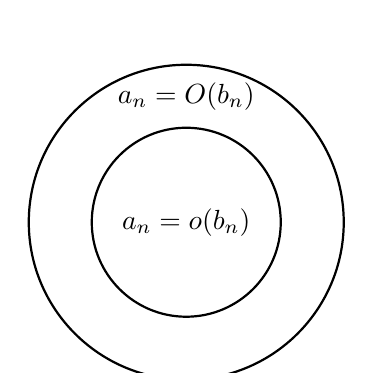
\begin{tikzpicture}
\draw[thick] (0,0) circle (2);
\draw[thick] (0,0) circle (1.2);
\node at (0,0) {$a_n = o(b_n)$};
\node at (0,1.6) {$a_n = O(b_n)$};
\end{tikzpicture}
\end{center}
\end{custom}

\begin{custom}{无穷小与无穷大的关系}
若 \(\{a_n\}\) 是非零无穷小量，则 \(\left\{\dfrac{1}{a_n}\right\}\) 是无穷大量；反之亦然。
\end{custom}

\begin{example}[常见无穷小量的比较]
当 \(n \to \infty\) 时：
\begin{itemize}
\item \(\dfrac{1}{n^p}\)（\(p>0\)）：\(p\) 越大，趋近 0 越快。
\item \(q^n\)（\(0 < q < 1\)）：指数衰减，比任何多项式都快。
\item \(\dfrac{1}{\ln n}\)：衰减极慢。
\item \(\dfrac{1}{n!}\)：衰减极快。
\end{itemize}

\textbf{增长率比较：} 当 \(n \to \infty\) 时，
\[
\ln n \ \ll\ n^p \ \ll\ a^n \ \ll\ n! \ \ll\ n^n \qquad (p>0,\ a>1).
\]
即：对数函数 < 幂函数 < 指数函数 < 阶乘 < \(n^n\)。
\end{example}

\begin{extra}
\subsection*{柯西收敛准则（选读）}
\addcontentsline{toc}{subsection}{柯西收敛准则（选读）}
\begin{definition}[柯西列]
若对任意 \(\varepsilon > 0\)，存在 \(N\)，当 \(m,n > N\) 时 \(|a_m - a_n| < \varepsilon\)，则称 \(\{a_n\}\) 为柯西列。
\end{definition}
在实数集中，柯西列必收敛（这等价于实数的完备性）。柯西准则的好处是：判断收敛性时不需要知道极限值。
\end{extra}

\subsection*{练习题：数列极限的严格定义}
\addcontentsline{toc}{subsection}{练习题：数列极限的严格定义}

\begin{exercise}
用 \(\varepsilon\)-\(N\) 语言来说明这些数列的极限。
\begin{enumerate}
\item \(\lim\limits_{n\to\infty} \dfrac{3}{n} = 0\)
\item \(\lim\limits_{n\to\infty} \dfrac{1}{\sqrt{n}} = 0\)
\item \(\lim\limits_{n\to\infty} \dfrac{5n-2}{n+1} = 5\)
\end{enumerate}
\end{exercise}

\begin{exercise}
\begin{enumerate}
\item 如果数列 \(\{a_n\}\) 收敛，它的极限是否唯一？请简要说明理由。
\item 若 \(\lim\limits_{n\to\infty} a_n = 3\)，证明：存在正整数 \(N\)，使得当 \(n > N\) 时，\(a_n > 2\)。
\item 证明：若数列 \(\{a_n\}\) 收敛，则它必有界。（提示：取 \(\varepsilon = 1\)）
\end{enumerate}
\end{exercise}

\begin{exercise}
\begin{enumerate}
\item 判断下列数列是否为无穷小量：
   \[
   a_n = \dfrac{(-1)^n}{n},\quad b_n = \dfrac{n}{n+1},\quad c_n = 0.99^n,\quad d_n = \ln\left(1+\dfrac{1}{n}\right)
   \]
\item 判断下列数列是否为无穷大量：
   \[
   a_n = n^2,\quad b_n = (-1)^n n,\quad c_n = \ln n,\quad d_n = \dfrac{n^2}{n+1}
   \]
\item 若 \(\{a_n\}\) 是无穷小量且 \(a_n \neq 0\)，证明 \(\left\{\dfrac{1}{a_n}\right\}\) 是无穷大量。
\end{enumerate}
\end{exercise}

\begin{exercise}
用 \(\varepsilon\)-\(N\) 定义证明下列极限：
\begin{enumerate}
\item \(\lim\limits_{n\to\infty} \dfrac{\sin n}{n^2 + 1} = 0\)（提示：\(|\sin n| \leq 1\)）
\item \(\lim\limits_{n\to\infty} \dfrac{3n + \cos n}{2n - 1} = \dfrac{3}{2}\)（提示：先分拆，再放缩）
\end{enumerate}
\end{exercise}

\begin{exercise}
用 \(\varepsilon\)-\(N\) 定义证明：
\[
\lim_{n\to\infty} \left(\sqrt{n^2 + n} - n\right) = \dfrac{1}{2}.
\]
（提示：分子有理化后处理）
\end{exercise}

\begin{exercise}
设常数 \(c > 0\)，证明：
\[
\lim_{n\to\infty} \dfrac{n^c}{a^n} = 0 \quad (a > 1).
\]
（提示：当 \(n\) 足够大时，\(a^n\) 增长快于任何幂函数；可用二项式定理或取对数）
\end{exercise}

\begin{exercise}
证明下列数列发散（极限不存在）：
\begin{enumerate}
\item \(a_n = (-1)^n\)
\item \(a_n = \sin\left(\dfrac{n\pi}{2}\right)\)
\item \(a_n = n + (-1)^n n\)（提示：考虑偶子列和奇子列）
\end{enumerate}
\end{exercise}

\begin{exercise}
用 \(\varepsilon\)-\(N\) 定义证明：
\[
\lim_{n\to\infty} \dfrac{n^2 - 2n + 3}{2n^2 + 5} = \dfrac{1}{2}.
\]
要求明确给出 \(N\) 关于 \(\varepsilon\) 的表达式（可分段处理）。
\end{exercise}

\begin{exercise}
用 \(\varepsilon\)-\(N\) 定义证明：
\begin{enumerate}
\item \(\lim\limits_{n\to\infty} \dfrac{\ln n}{n} = 0\)（提示：对任意 \(\varepsilon > 0\)，取 \(N = \lceil e^{1/\varepsilon} \rceil\) 是否可行？需要调整）
\item \(\lim\limits_{n\to\infty} \sqrt[n]{n} = 1\)（提示：设 \(\sqrt[n]{n} = 1 + h_n\)，利用二项式定理证明 \(h_n \to 0\)）
\end{enumerate}
\end{exercise}

\begin{exercise}
设 \(a_n = \dfrac{1}{n^2 + 1} + \dfrac{1}{n^2 + 2} + \cdots + \dfrac{1}{n^2 + n}\)。
\begin{enumerate}
\item 证明：\(\dfrac{n}{n^2 + n} \leq a_n \leq \dfrac{n}{n^2 + 1}\)。
\item 利用夹逼准则求 \(\lim\limits_{n\to\infty} a_n\)。
\item 用 \(\varepsilon\)-\(N\) 定义直接证明该极限。（选做）
\end{enumerate}
\end{exercise}

\begin{exercise}[*（柯西收敛准则）]
设数列 \(\{a_n\}\) 满足：对任意 \(n\)，有 \(|a_{n+1} - a_n| \leq \dfrac{1}{2^n}\)。
\begin{enumerate}
\item 证明：对任意 \(m > n\)，有 \(|a_m - a_n| \leq \dfrac{1}{2^{n-1}}\)。（提示：用三角不等式和等比数列求和）
\item 证明：\(\{a_n\}\) 是柯西列，从而收敛。
\item 若已知 \(a_1 = 1\)，能否求出 \(\lim\limits_{n\to\infty} a_n\)？为什么？
\end{enumerate}
\end{exercise}


\subsection*{参考答案提要}
\addcontentsline{toc}{subsection}{参考答案提要}

\begin{enumerate}
\item[(1)] 
   (a) \(N = \lceil 3/\varepsilon \rceil\)；(b) \(N = \lceil 1/\varepsilon^2 \rceil\)；(c) \(\left|\dfrac{5n-2}{n+1} - 5\right| = \dfrac{7}{n+1}\)，取 \(N = \lceil 7/\varepsilon \rceil\)。

\item[(2)] 
   (a) 唯一，反证法用 \(\varepsilon = |L_1 - L_2|/2\) 导出矛盾；(b) 取 \(\varepsilon = 1\)，存在 \(N\) 使 \(n > N\) 时 \(|a_n-3|<1\)，故 \(a_n > 2\)；(c) 取 \(\varepsilon=1\)，有界性证明略。

\item[(3)] 
   (a) 无穷小量：\(a_n, c_n, d_n\)（\(b_n \to 1\) 不是）；(b) 无穷大量：\(a_n, c_n, d_n\)（\(b_n\) 无界但不趋于无穷）；(c) 由定义直接验证。

\item[(4)] 
   (a) \(\left|\dfrac{\sin n}{n^2+1}\right| \leq \dfrac{1}{n^2}\)，取 \(N = \lceil 1/\sqrt{\varepsilon} \rceil\)；(b) 先化简为 \(\dfrac{3}{2} + \dfrac{3\cos n + 3/2}{2(2n-1)}\) 再放缩。

\item[(5)] 
   分子有理化：\(\sqrt{n^2+n} - n = \dfrac{n}{\sqrt{n^2+n}+n} = \dfrac{1}{\sqrt{1+1/n}+1}\)，然后放缩证明。

\item[(6)] 
   令 \(a_n = n^c / a^n\)，当 \(n > 2c\) 时可用二项式定理 \((1+(a-1))^n \geq \binom{n}{2}(a-1)^2\) 放缩。

\item[(7)] 
   (a) 子列极限不同；(b) 子列 \(0,1,0,-1,\dots\) 不收敛；(c) \(a_n = n(1+(-1)^n)\)，偶数项 \(\to +\infty\)，奇数项为 0。

\item[(8)] 
   \(\left|\dfrac{n^2-2n+3}{2n^2+5} - \dfrac{1}{2}\right| = \dfrac{4n+1}{2(2n^2+5)} < \dfrac{4n+1}{4n^2} < \dfrac{5}{4n}\)（当 \(n \geq 1\)），取 \(N = \lceil 5/(4\varepsilon) \rceil\)。

\item[(9)] 
   (a) 取 \(N = \lceil e^{2/\varepsilon} \rceil\) 或通过 \(n > e^{1/\varepsilon}\) 放缩；(b) 由 \(\sqrt[n]{n} = 1+h_n\)，二项展开得 \(n = (1+h_n)^n \geq \binom{n}{2}h_n^2\)，故 \(h_n^2 \leq \dfrac{2}{n-1} \to 0\)。

\item[(10)] 
   (a) 左边放缩：每项 \(\geq \dfrac{1}{n^2+n}\)，共 \(n\) 项；右边放缩：每项 \(\leq \dfrac{1}{n^2+1}\)；(b) 夹逼得极限为 0；(c) 直接证明：\(0 \leq a_n \leq \dfrac{1}{n}\)，取 \(N = \lceil 1/\varepsilon \rceil\)。

\item[(11)] 
   (a) \(|a_m - a_n| \leq \sum_{k=n}^{m-1} |a_{k+1}-a_k| \leq \sum_{k=n}^{\infty} \dfrac{1}{2^k} = \dfrac{1}{2^{n-1}}\)；(b) 由 (a) 知 \(\{a_n\}\) 是柯西列，故收敛；(c) 不能，因为只知道差值大小，不知道具体值。
\end{enumerate}

\clearpage
\section{极限的性质与重要极限}

\subsection{收敛数列的基本性质}

\begin{theorem}[极限的性质]
设 \(\{a_n\}, \{b_n\}\) 为收敛数列。
\begin{enumerate}
\item \textbf{唯一性：} 收敛数列极限唯一。
\item \textbf{保号性：} 若当 \(n\) 充分大时 \(a_n \geq 0\)，且 \(\lim a_n = L\)，则 \(L \geq 0\)。
\item \textbf{有界性：} 收敛数列必有界。
\item \textbf{夹逼准则（三明治定理）：} 若 \(b_n \leq a_n \leq c_n\)（当 \(n\) 充分大）且 \(\lim b_n = \lim c_n = L\)，则 \(\lim a_n = L\)。
\item \textbf{四则运算：}
   \begin{align*}
   \lim (c_1 a_n + c_2 b_n) &= c_1 \lim a_n + c_2 \lim b_n,\\
   \lim (a_n b_n) &= (\lim a_n)(\lim b_n),\\
   \lim \dfrac{a_n}{b_n} &= \dfrac{\lim a_n}{\lim b_n} \quad (\lim b_n \neq 0).
   \end{align*}
\end{enumerate}
\end{theorem}

\begin{custom}{唯一性的证明}
假设 \(a_n \to L_1\) 且 \(a_n \to L_2\)。对任意 \(\varepsilon > 0\)，存在 \(N_1, N_2\) 使当 \(n > \max(N_1, N_2)\) 时，
\[
|a_n - L_1| < \varepsilon,\quad |a_n - L_2| < \varepsilon.
\]
于是
\[
|L_1 - L_2| \leq |L_1 - a_n| + |a_n - L_2| < 2\varepsilon.
\]
由于 \(\varepsilon\) 可以任意小，而 \(|L_1 - L_2|\) 是常数，故 \(L_1 = L_2\)。\(\square\)
\end{custom}

\begin{custom}{保号性的证明}
假设 \(\lim a_n = L < 0\)。取 \(\varepsilon = -L/2 > 0\)，则存在 \(N\)，当 \(n > N\) 时 \(|a_n - L| < -L/2\)，从而 \(a_n < L/2 < 0\)，与 \(a_n \geq 0\) 矛盾。故 \(L \geq 0\)。\(\square\)
\end{custom}

\begin{custom}{有界性的证明}
设 \(\lim a_n = L\)。取 \(\varepsilon = 1\)，存在 \(N\)，当 \(n > N\) 时 \(|a_n - L| < 1\)，故 \(|a_n| < |L| + 1\)。取
\[
M = \max\{|a_1|, |a_2|, \dots, |a_N|, |L|+1\},
\]
则对所有 \(n\) 有 \(|a_n| \leq M\)。\(\square\)
\end{custom}

\begin{custom}{夹逼准则的证明}
由 \(\lim b_n = L\)，对 \(\varepsilon > 0\)，存在 \(N_1\) 使 \(n > N_1\) 时 \(L - \varepsilon < b_n < L + \varepsilon\)。
由 \(\lim c_n = L\)，存在 \(N_2\) 使 \(n > N_2\) 时 \(L - \varepsilon < c_n < L + \varepsilon\)。
取 \(N = \max(N_1, N_2)\)，则当 \(n > N\) 时，
\[
L - \varepsilon < b_n \leq a_n \leq c_n < L + \varepsilon,
\]
故 \(|a_n - L| < \varepsilon\)，即 \(\lim a_n = L\)。\(\square\)
\end{custom}

\begin{custom}{四则运算的证明思路}
以乘法为例：设 \(a_n \to A\)，\(b_n \to B\)。则
\[
a_n b_n - AB = (a_n - A)b_n + A(b_n - B).
\]
由于 \(b_n\) 有界，\(a_n - A \to 0\)，故第一项趋于 0；第二项也趋于 0。因此 \(a_n b_n \to AB\)。
\end{custom}

\subsection{Landau 符号的四则运算性质}

在极限计算和渐近分析中，小 \(o\) 和大 \(O\) 记号具有简洁的运算规则，掌握这些规则可以极大地简化极限计算。

\begin{theorem}[小 \(o\) 与大 \(O\) 的运算性质]
设 \(f(x), g(x), h(x)\) 是定义在某个邻域内的函数（或数列），且 \(x \to x_0\)（或 \(n \to \infty\)）。则以下运算规则成立：

\begin{enumerate}
\item \textbf{常数倍：}
   \[
   c \cdot o(g) = o(g),\quad c \cdot O(g) = O(g) \quad (c \text{ 为非零常数})
   \]

\item \textbf{加减法：}
   \[
   o(g) + o(g) = o(g),\quad O(g) + O(g) = O(g)
   \]
   \[
   o(g) - o(g) = o(g),\quad O(g) - O(g) = O(g)
   \]
   \[
   o(g) + O(g) = O(g) \quad (\text{但通常不能写成 } o(g))
   \]

\item \textbf{乘法：}
   \[
   o(g) \cdot o(h) = o(gh),\quad O(g) \cdot O(h) = O(gh)
   \]
   \[
   o(g) \cdot O(h) = o(gh),\quad O(g) \cdot o(h) = o(gh)
   \]

\item \textbf{传递性：}
   \begin{itemize}
   \item 若 \(f = o(g)\) 且 \(g = o(h)\)，则 \(f = o(h)\)
   \item 若 \(f = O(g)\) 且 \(g = O(h)\)，则 \(f = O(h)\)
   \item 若 \(f = o(g)\) 且 \(g = O(h)\)，则 \(f = o(h)\)
   \end{itemize}

\item \textbf{与极限的关系：}
   \begin{itemize}
   \item \(f(x) \to 0\) 当且仅当 \(f(x) = o(1)\)
   \item \(f(x)\) 有界当且仅当 \(f(x) = O(1)\)
   \end{itemize}

\item \textbf{主要项法则：} 若 \(f = o(g)\)，则 \(f + g \sim g\)（即 \(f+g\) 与 \(g\) 是等价无穷小）
\end{enumerate}
\end{theorem}

\begin{custom}{规则背后的直观理解}

这些规则其实很符合直觉：

\begin{itemize}
\item \textbf{加法规则：} 两个“小东西”加起来还是“小东西”；两个“有界的东西”加起来还是有界的。
\item \textbf{乘法规则：} “小东西”乘以“小东西”更小（高阶乘高阶得更高阶）；“小东西”乘以“有界的东西”还是小东西。
\item \textbf{传递性：} 如果 \(f\) 比 \(g\) 小得多，\(g\) 比 \(h\) 小得多，那么 \(f\) 比 \(h\) 小得多。
\end{itemize}

\textbf{一个容易混淆的点：} \(o(g) + O(g) = O(g)\)，但不能写成 \(o(g)\)。因为 \(O(g)\) 可能包含一个与 \(g\) 同阶的项（比如 \(g\) 本身），而 \(o(g)\) 要求比值趋于 0，所以 \(g\) 本身不是 \(o(g)\)。
\end{custom}


\begin{example}[利用 o 和 O 比较数列增长]
比较下列数列的增长速度：
\[
a_n = n^2 + n \ln n,\quad b_n = n^2.
\]

\begin{custom}{解}
\[
a_n = n^2 + n \ln n = n^2 \left(1 + \dfrac{\ln n}{n}\right).
\]
由于 \(\dfrac{\ln n}{n} = o(1)\)，所以
\[
a_n = n^2 (1 + o(1)) = n^2 + o(n^2).
\]
因此 \(a_n \sim n^2\)，即 \(a_n\) 与 \(b_n\) 是等价无穷大（当 \(n \to \infty\)）。
\end{custom}
\end{example}

\begin{custom}{常见错误警示}

\begin{center}
\small
\begin{tabularx}{\textwidth}{|>{\raggedright\arraybackslash}X|>{\raggedright\arraybackslash}X|>{\raggedright\arraybackslash}X|}
\hline
\textbf{错误写法} & \textbf{问题} & \textbf{正确理解} \\
\hline
\(o(g) - o(g) = 0\) & 两个不同的 \(o(g)\) 相减不一定为 0 & \(o(g) - o(g) = o(g)\) \\
\hline
\(\dfrac{o(g)}{g} = 0\) & 写法不规范 & 应写为 \(\dfrac{o(g)}{g} \to 0\) \\
\hline
\(o(1) \cdot \infty = ?\) & 未定义 & \(o(1)\) 乘以无穷大可能为任何情况 \\
\hline
\(\sin x = x + O(x^3)\) 与 \(\sin x = x + o(x^2)\) 混淆 & 精度不同 & \(O(x^3)\) 比 \(o(x^2)\) 提供更多信息 \\
\hline
\end{tabularx}
\end{center}

\textbf{核心原则：} 小 \(o\) 描述的是“比……高阶”，大 \(O\) 描述的是“不超过……的常数倍”。在运算中，小 \(o\) 会“吸收”比自己低阶或同阶的项，而大 \(O\) 只保证有界性。
\end{custom}

\subsection{极限存在性定理}

有时候我们不知道极限值，但仍能判断极限是否存在。

\begin{theorem}[单调有界准则]
单调递增且有上界的数列必收敛；单调递减且有下界的数列必收敛。
\end{theorem}

\begin{custom}{证明}
只证明单调递增且有上界的情形，单调递减且有下界的情形可令 $b_n=-a_n$ 化为前一情形.

设 $\{a_n\}$ 单调递增且有上界. 由实数完备性，集合
\[
A=\{a_n:n=1,2,\ldots\}
\]
存在上确界，记为 $\alpha=\sup A$. 下面证明 $a_n\to\alpha$.

任取 $\varepsilon>0$. 因 $\alpha$ 是 $A$ 的上确界，$\alpha-\varepsilon$ 不是 $A$ 的上界，否则它会小于上确界却仍为上界，与上确界定义矛盾. 因此存在某个正整数 $N$，使得
\[
a_N>\alpha-\varepsilon.
\]
又因数列单调递增，当 $n\ge N$ 时有
\[
a_n\ge a_N>\alpha-\varepsilon.
\]
同时 $\alpha$ 是上界，故 $a_n\le \alpha$. 于是当 $n\ge N$ 时，
\[
0\le \alpha-a_n<\varepsilon,
\]
即 $|a_n-\alpha|<\varepsilon$. 由数列极限定义，$a_n\to\alpha$.
\end{custom}

\begin{custom}{直观理解}
想象一个人在数轴上向右走（单调递增），但前面有一堵墙（上界）。他不能无限向右，只能越来越靠近某个点。这个点就是极限。
\end{custom}

\begin{example}[重要例子]
证明数列 \(a_1 = \sqrt{2}\)，\(a_{n+1} = \sqrt{2 + a_n}\) 收敛并求极限。
\end{example}
\begin{custom}{解}
\textbf{有界性：} \(a_1 = \sqrt{2} < 2\)，假设 \(a_k < 2\)，则 \(a_{n+1} = \sqrt{2 + a_n} < \sqrt{4} = 2\)，故 \(a_n < 2\) 对所有 \(n\) 成立。
\textbf{单调性：} \(a_2 = \sqrt{2+\sqrt{2}} > \sqrt{2} = a_1\)，假设 \(a_k > a_{k-1}\)，则 \(a_{k+1} = \sqrt{2 + a_k} > \sqrt{2 + a_{k-1}} = a_k\)，故 \(\{a_n\}\) 严格递增。
由单调有界准则，极限存在。设 \(\lim a_n = L\)，在递推式两边取极限：
\[
L = \sqrt{2 + L} \quad\Longrightarrow\quad L^2 = L + 2 \quad\Longrightarrow\quad L = 2\ (\text{舍去 } -1).
\]
\end{custom}

\begin{theorem}[Bolzano-Weierstrass定理]
\textbf{（有界数列必有收敛子列）}
任何有界数列 \(\{a_n\}\) 必定存在一个收敛的子列 \(\{a_{n_k}\}\)。
\end{theorem}

\begin{custom}{证明}
设 $\{a_n\}$ 有界，则存在闭区间 $I_0=[\alpha_0,\beta_0]$ 包含数列的全部项. 将 $I_0$ 等分为左右两个闭区间. 至少有一个半区间包含数列中的无穷多项；否则两个半区间都只含有限多项，合起来也只含有限多项，与原数列有无穷多项矛盾. 取其中一个含无穷多项的半区间记为 $I_1$.

继续这个过程：把 $I_{k-1}$ 等分，取一个包含数列中无穷多项的半区间 $I_k$. 得到一列闭区间
\[
I_0\supset I_1\supset I_2\supset\cdots,\qquad |I_k|=\frac{|I_0|}{2^k}.
\]
根据闭区间套定理，存在唯一实数 $\xi$ 属于所有 $I_k$，并且区间长度趋于 $0$.

下面从数列中选子列. 因 $I_1$ 含无穷多项，可取 $n_1$ 使 $a_{n_1}\in I_1$. 取定 $n_1,\ldots,n_{k-1}$ 后，由于 $I_k$ 含无穷多项，可选 $n_k>n_{k-1}$ 使 $a_{n_k}\in I_k$. 于是得到子列 $\{a_{n_k}\}$.

任取 $\varepsilon>0$. 因 $|I_k|\to0$，存在 $K$，当 $k\ge K$ 时 $|I_k|<\varepsilon$. 对 $k\ge K$，$a_{n_k}$ 与 $\xi$ 同属 $I_k$，故
\[
|a_{n_k}-\xi|\le |I_k|<\varepsilon.
\]
由极限定义，$a_{n_k}\to\xi$. 因此有界数列必有收敛子列.
\end{custom}

\begin{custom}{直观理解}

这个定理说的是：如果你有一列数，它们都挤在某个有限的区间里（比如都在 \([-M, M]\) 之间），那么无论它们看起来多么杂乱无章，你总能从中挑出一个“收敛”的子序列。

\textbf{一个生活中的比喻：}

想象一个无限大的体育馆里有无穷多个人，每个人手里拿着一个数字，所有数字都在 0 到 1 之间。你想找出一群人，他们手里的数字越来越接近某个固定值。

Bolzano-Weierstrass 定理保证：你一定能找到这样一群人！无论这些人怎么站队，你总能挑出一个子序列，它最终会稳定在某个数附近。

\textbf{一个更直观的几何解释：}

把数列 \(\{a_n\}\) 想象成数轴上的无限个点，所有点都被关在区间 \([-M, M]\) 这个“笼子”里。

\begin{center}
\begin{tikzpicture}[scale=0.8]
\draw[thick, -{Stealth}] (-5,0) -- (5,0) node[right] {数轴};
\draw[thick] (-4,0.1) -- (-4,-0.1) node[below] {\(-M\)};
\draw[thick] (4,0.1) -- (4,-0.1) node[below] {\(M\)};
\draw[thick, red] (-4,0.2) -- (4,0.2) node[above] {笼子（有界区间）};

\foreach \x in {-3.2, -1.5, -0.8, 0.3, 1.2, 2.5, 3.7, -2.1, 0.9, 2.8, -0.2, 1.9, -2.9, 3.1} {
    \filldraw[blue] (\x,0) circle (2pt);
}
\end{tikzpicture}
\end{center}

\textbf{核心思想——二分法：}

你可以用“不断对半分割区间”的方法来构造这个收敛子列：

\begin{enumerate}
\item 一开始，所有点都在区间 \([a, b] = [-M, M]\) 里。
\item 把这个区间分成两半：左边 \([-M, 0]\) 和右边 \([0, M]\)。由于有无穷多个点，至少有一半包含无穷多个点。选择那一半作为新区间 \([a_1, b_1]\)。
\item 再把新区间对半分，同样，至少有一半包含无穷多个点。选择那一半作为 \([a_2, b_2]\)。
\item 如此无限继续下去，我们得到一列不断缩小的区间：
\[
[a, b] \supset [a_1, b_1] \supset [a_2, b_2] \supset \cdots
\]
\item 每次区间的长度减半：\(b_n - a_n = \dfrac{2M}{2^n} \to 0\)。
\item 从每个区间里选出一个数列中的点 \(a_{n_k}\)，这些点就构成了一个收敛的子列。这些点被“挤压”在越来越小的区间里，最终会收敛到区间的公共极限点 \(c\)。
\end{enumerate}

\textbf{一个具体的例子：}

考虑数列 \(a_n = \sin n\)。虽然 \(\sin n\) 在 \([-1, 1]\) 之间振荡，看起来毫无规律，但 Bolzano-Weierstrass 定理告诉我们：一定存在一个子列收敛。事实上，可以证明 \(\sin n\) 的子列可以收敛到 \([-1, 1]\) 中的任意值，但这个定理只保证“存在”，不告诉我们具体是哪个。

\end{custom}

\begin{custom}{单调有界准则 vs Bolzano-Weierstrass 定理}

这两个定理是实数完备性的不同表现形式，它们实际上是等价的（在实数系中可以互相推导）。

\begin{tabular}{|c|c|c|}
\hline
 & \textbf{单调有界准则} & \textbf{Bolzano-Weierstrass 定理} \\
\hline
\textbf{条件} & 数列单调 + 有界 & 数列有界（不要求单调） \\
\hline
\textbf{结论} & 数列本身收敛 & 存在收敛子列 \\
\hline
\textbf{适用场景} & 单调数列 & 任意有界数列 \\
\hline
\textbf{直观比喻} & 向右走，前面有墙 & 笼子里的无限多只鸟 \\
\hline
\end{tabular}

\textbf{关系：}
\begin{itemize}
\item 单调有界准则更强：它直接得出数列本身收敛。
\item Bolzano-Weierstrass 更广：它适用于任何有界数列，但只给出子列收敛。
\item 如果数列既有界又单调，两个定理都适用，但单调有界准则给出的结论更强。
\end{itemize}

\end{custom}


\begin{example}[重要例子]
证明数列 \(a_1 = \sqrt{2}\)，\(a_{n+1} = \sqrt{2 + a_n}\) 收敛并求极限。
\end{example}
\begin{custom}{解}
\textbf{有界性：} \(a_1 = \sqrt{2} < 2\)，假设 \(a_k < 2\)，则 \(a_{k+1} = \sqrt{2 + a_k} < \sqrt{4} = 2\)，故 \(a_n < 2\) 对所有 \(n\) 成立。
\textbf{单调性：} \(a_2 = \sqrt{2+\sqrt{2}} > \sqrt{2} = a_1\)，假设 \(a_k > a_{k-1}\)，则 \(a_{k+1} = \sqrt{2 + a_k} > \sqrt{2 + a_{k-1}} = a_k\)，故 \(\{a_n\}\) 严格递增。
由单调有界准则，极限存在。设 \(\lim a_n = L\)，在递推式两边取极限：
\[
L = \sqrt{2 + L} \quad\Longrightarrow\quad L^2 = L + 2 \quad\Longrightarrow\quad L = 2\ (\text{舍去 } -1).
\]
\end{custom}

\subsection{两个重要极限}

\begin{theorem}[第一个重要极限]
\[
\lim_{n\to\infty} \left(1 + \dfrac{1}{n}\right)^n = e.
\]
\end{theorem}

\textbf{故事背景：} 17世纪，数学家雅各布·伯努利在研究复利问题时遇到了这个极限。假设你存 1 元钱，年利率 100\%，如果一年计一次息，本息和为 2 元；如果半年计一次，本息和为 \((1+0.5)^2 = 2.25\)；如果每月计一次，为 \((1+1/12)^{12} \approx 2.613\)；如果每天计一次，约为 \(2.71457\)。这个数的极限就是 \(e \approx 2.71828\ldots\)。

\begin{custom}{具体证明}
证明分为两步：先证 \(\{a_n\}\) 单调递增，再证它有上界。

\noindent\textbf{第一步：证明单调递增}

由二项式定理展开：
\[
a_n = \left(1+\dfrac{1}{n}\right)^n = \sum_{k=0}^{n} C_n^k \dfrac{1}{n^k} = \sum_{k=0}^{n} \dfrac{1}{k!} \cdot \dfrac{n(n-1)\cdots(n-k+1)}{n^k}.
\]
其中 \(\dfrac{n(n-1)\cdots(n-k+1)}{n^k} = 1 \cdot \left(1-\dfrac{1}{n}\right) \cdots \left(1-\dfrac{k-1}{n}\right)\)。于是
\[
a_n = \sum_{k=0}^{n} \dfrac{1}{k!} \left(1-\dfrac{1}{n}\right)\left(1-\dfrac{2}{n}\right)\cdots\left(1-\dfrac{k-1}{n}\right).
\]

同理，
\[
a_{n+1} = \sum_{k=0}^{n+1} \dfrac{1}{k!} \left(1-\dfrac{1}{n+1}\right)\left(1-\dfrac{2}{n+1}\right)\cdots\left(1-\dfrac{k-1}{n+1}\right).
\]

比较 \(a_n\) 与 \(a_{n+1}\) 中 \(k\) 相同的项（\(1 \leq k \leq n\)）：
\[
\left(1-\dfrac{1}{n}\right)\left(1-\dfrac{2}{n}\right)\cdots\left(1-\dfrac{k-1}{n}\right) < \left(1-\dfrac{1}{n+1}\right)\left(1-\dfrac{2}{n+1}\right)\cdots\left(1-\dfrac{k-1}{n+1}\right),
\]
因为每个因子 \(1-\dfrac{j}{n} < 1-\dfrac{j}{n+1}\)（\(j=1,2,\dots,k-1\)）。同时 \(a_{n+1}\) 比 \(a_n\) 多一项正的 \(\dfrac{1}{(n+1)!}\)。因此
\[
a_n < a_{n+1},
\]
故数列严格递增。

\noindent\textbf{第二步：证明有上界}

由展开式，
\[
a_n = \sum_{k=0}^{n} \dfrac{1}{k!} \left(1-\dfrac{1}{n}\right)\cdots\left(1-\dfrac{k-1}{n}\right) < \sum_{k=0}^{n} \dfrac{1}{k!}.
\]

当 \(k \geq 1\) 时，\(k! = 1 \cdot 2 \cdot 3 \cdots k \geq 1 \cdot 2 \cdot 2 \cdots 2 = 2^{k-1}\)，因此
\[
\dfrac{1}{k!} \leq \dfrac{1}{2^{k-1}} \quad (k \geq 1).
\]

于是
\[
a_n < 1 + 1 + \dfrac{1}{2} + \dfrac{1}{2^2} + \cdots + \dfrac{1}{2^{n-1}} = 1 + \dfrac{1 - (1/2)^n}{1 - 1/2} = 1 + 2\left(1 - \dfrac{1}{2^n}\right) < 3.
\]

所以 \(a_n < 3\) 对所有 \(n\) 成立，数列有上界。

\noindent\textbf{结论：} 数列 \(\{a_n\}\) 单调递增且有上界，由单调有界准则，极限存在。记这个极限为 \(e\)，即
\[
e = \lim_{n\to\infty} \left(1+\dfrac{1}{n}\right)^n.
\]
\end{custom}

\begin{theorem}[第一个重要极限的推广]
\[
\lim_{n\to\infty} \left(1 + \dfrac{a}{n}\right)^n = e^a.
\]
特别地，\(\lim_{x\to 0} (1+x)^{1/x} = e\)。
\end{theorem}

\subsection{重要极限 \(\lim_{x \to 0} \dfrac{\sin x}{x} = 1\)}

这个极限是微积分中最重要的极限之一。它告诉我们：当 \(x\) 非常接近 0 时，\(\sin x\) 和 \(x\) 几乎相等。

\begin{custom}{几何直观：从单位圆看起}

画一个半径为 1 的圆（单位圆）。在圆中取一个很小的角 \(x\)，如图：

\begin{center}
\begin{tikzpicture}[scale=3]
\draw[->] (-0.2,0) -- (1.2,0) node[right] {$x$};
\draw[->] (0,-0.2) -- (0,1.2) node[above] {$y$};
\draw (0,0) circle (1);
\draw (0,0) -- (1,0) node[right] {$A$};
\draw (0,0) -- ({cos(30)},{sin(30)}) node[above right] {$B$};
\draw (1,0) -- ({cos(30)},{sin(30)});
\draw ({cos(0.8)},0) -- ({cos(30)},{sin(30)});
\draw (0.4,0) arc (0:45:0.4);
\node at (0.25,0.12) {$x$};
\node at (0.5,0.1) {$\tan x$};
\node at (1.05,0.55) {$\sin x$};
\node at (0.5,-0.08) {$\cos x$};
\end{tikzpicture}
\end{center}

图中：
\begin{itemize}
\item 角 \(x\) 对应的圆弧长 = \(x\)（因为半径=1，弧长=半径×角度）
\item 垂线 \(BC\) 的长度 = \(\sin x\)
\item 水平线 \(AC\) 的长度 = \(\cos x\)
\item 切线 \(AD\) 的长度 = \(\tan x\)
\end{itemize}

从图中可以看出，三个面积之间有如下关系：

\[
\triangle OAB \text{ 的面积 } < \text{ 扇形 } OAB \text{ 的面积 } < \triangle OAD \text{ 的面积}.
\]

\end{custom}

\begin{custom}{面积比较}

\begin{itemize}
\item \(\triangle OAB\) 的面积 = \(\dfrac{1}{2} \times 1 \times \sin x = \dfrac{1}{2} \sin x\)
\item 扇形 \(OAB\) 的面积 = \(\dfrac{1}{2} \times 1^2 \times x = \dfrac{x}{2}\)
\item \(\triangle OAD\) 的面积 = \(\dfrac{1}{2} \times 1 \times \tan x = \dfrac{1}{2} \tan x\)
\end{itemize}

因此：

\[
\dfrac{1}{2} \sin x  <  \dfrac{x}{2} < \dfrac{1}{2} \tan x \qquad (0 < x < \dfrac{\pi}{2}).
\]

两边同时乘以 2，得到：

\[
\sin x  < x < \tan x.
\]

\end{custom}

\begin{custom}{推导 \(\dfrac{\sin x}{x}\) 的夹逼不等式}

由 \(x < \tan x = \dfrac{\sin x}{\cos x}\)，两边同时除以 \(\sin x > 0\)，得：

\[
\dfrac{x}{\sin x} < \dfrac{1}{\cos x} \quad \Longrightarrow \quad \cos x < \dfrac{\sin x}{x}.
\]

又由 \(\sin x < x\)，两边除以 \(x > 0\)，得：

\[
\dfrac{\sin x}{x} < 1.
\]

合起来：

\[
\cos x < \dfrac{\sin x}{x} < 1 \qquad (0 < x < \dfrac{\pi}{2}).
\]

\end{custom}

\begin{custom}{用夹逼准则取极限}

我们知道 \(\lim_{x \to 0} \cos x = 1\)。因此，当 \(x \to 0^+\) 时：

\[
\cos x \;\longrightarrow\; 1,\quad \dfrac{\sin x}{x} \;\longrightarrow\; 1.
\]

当 \(x\) 为负时（即 \(x \to 0^-\)），由于 \(\dfrac{\sin x}{x}\) 是偶函数（\(\sin(-x)/(-x) = \sin x / x\)），左右极限相等。因此：

\[
\lim_{x \to 0} \dfrac{\sin x}{x} = 1.
\]

\end{custom}

\begin{custom}{直观理解}

这个极限告诉我们：当角度 \(x\) 非常小时，\(\sin x\) 和 \(x\) 几乎相等。例如：

\[
x = 0.1 \text{ 弧度} \approx 5.73^\circ,\quad \sin(0.1) \approx 0.099833,\quad \dfrac{\sin 0.1}{0.1} \approx 0.99833.
\]

\[
x = 0.01 \text{ 弧度},\quad \dfrac{\sin 0.01}{0.01} \approx 0.999983.
\]

误差非常小，且随 \(x\) 越小越接近 1。

\end{custom}

\subsection{等价无穷小}

在计算极限时，我们经常遇到两个无穷小量相乘或相除的情况。如果能用一个简单的无穷小量代替复杂的无穷小量，计算会大大简化。这就是等价无穷小的思想。

\begin{definition}[等价无穷小]
设当 \(x \to x_0\)（或 \(x \to \infty\)）时，\(\alpha(x) \to 0\)，\(\beta(x) \to 0\)，且
\[
\lim \dfrac{\alpha(x)}{\beta(x)} = 1,
\]
则称 \(\alpha(x)\) 与 \(\beta(x)\) 是等价无穷小，记作 \(\alpha(x) \sim \beta(x)\)。
\end{definition}

\begin{custom}{直观理解}
等价无穷小意味着：当两个量都趋近于 0 时，它们的比值趋近于 1，即它们“以相同的速度”趋近于 0。

打个比方：两辆赛车同时冲向终点，如果它们速度相同，那么它们之间的距离会越来越小，最终几乎同时到达。等价无穷小就是这种“同步趋近”的数学描述。
\end{custom}

\subsection{常用等价无穷小（\(x \to 0\) 时）}

以下等价关系是微积分中最常用的，务必熟记：

\[
\boxed{
\begin{aligned}
\sin x &\sim x & \tan x &\sim x \\
\arcsin x &\sim x & \arctan x &\sim x \\
e^x - 1 &\sim x & \ln(1+x) &\sim x \\
1 - \cos x &\sim \dfrac{x^2}{2} & (1+x)^a - 1 &\sim ax \quad (a \neq 0)
\end{aligned}
}
\]

\begin{custom}{几个等价关系的推导}

\begin{itemize}
\item \textbf{\(\sin x \sim x\)：} 这就是我们之前证明的 \(\lim_{x \to 0} \dfrac{\sin x}{x} = 1\)。

\item \textbf{\(\tan x \sim x\)：} 
\[
\lim_{x \to 0} \dfrac{\tan x}{x} = \lim_{x \to 0} \dfrac{\sin x}{x} \cdot \dfrac{1}{\cos x} = 1 \cdot 1 = 1.
\]

\item \textbf{\(e^x - 1 \sim x\)：} 令 \(t = e^x - 1\)，则 \(x = \ln(1+t)\)，当 \(x \to 0\) 时 \(t \to 0\)，
\[
\lim_{x \to 0} \dfrac{e^x - 1}{x} = \lim_{t \to 0} \dfrac{t}{\ln(1+t)} = 1.
\]

\item \textbf{\(\ln(1+x) \sim x\)：} 
\[
\lim_{x \to 0} \dfrac{\ln(1+x)}{x} = \lim_{x \to 0} \ln(1+x)^{1/x} = \ln e = 1.
\]

\item \textbf{\(1 - \cos x \sim \dfrac{x^2}{2}\)：} 
\[
\lim_{x \to 0} \dfrac{1 - \cos x}{x^2/2} = \lim_{x \to 0} \dfrac{2 \sin^2(x/2)}{x^2/2} = \lim_{x \to 0} \dfrac{4 \sin^2(x/2)}{x^2} = \lim_{x \to 0} \left(\dfrac{\sin(x/2)}{x/2}\right)^2 = 1.
\]

\item \textbf{\((1+x)^a - 1 \sim ax\)：} 
\[
\lim_{x \to 0} \dfrac{(1+x)^a - 1}{ax} = \dfrac{1}{a} \cdot \lim_{x \to 0} \dfrac{e^{a\ln(1+x)} - 1}{x} = \dfrac{1}{a} \cdot \lim_{x \to 0} \dfrac{a\ln(1+x)}{x} = 1.
\]
\end{itemize}
\end{custom}

\subsection{等价无穷小的应用：简化极限计算}

\begin{custom}{核心原则}
在乘除结构中，可以用等价无穷小替换来简化计算：
\[
\lim \dfrac{f(x)}{g(x)} = \lim \dfrac{\tilde{f}(x)}{\tilde{g}(x)},
\]
其中 \(\tilde{f} \sim f\)，\(\tilde{g} \sim g\)。

\textbf{但注意：} 在加减结构中，不能随意替换！因为主要项可能相互抵消，替换后可能丢失关键信息。
\end{custom}

\begin{example}[乘除结构中的替换]
求 \(\lim\limits_{x \to 0} \dfrac{\sin 2x \cdot \ln(1+3x)}{x^2}\)。
\end{example}
\begin{custom}{解}
当 \(x \to 0\) 时，\(\sin 2x \sim 2x\)，\(\ln(1+3x) \sim 3x\)，所以
\[
\dfrac{\sin 2x \cdot \ln(1+3x)}{x^2} \sim \dfrac{(2x) \cdot (3x)}{x^2} = 6 \quad \Rightarrow \quad \text{极限为 } 6.
\]
更严谨地：
\[
\lim_{x \to 0} \dfrac{\sin 2x \cdot \ln(1+3x)}{x^2} = \lim_{x \to 0} \dfrac{\sin 2x}{2x} \cdot \dfrac{\ln(1+3x)}{3x} \cdot 6 = 1 \cdot 1 \cdot 6 = 6.
\]
\end{custom}

\begin{example}[乘除结构中的复杂替换]
求 \(\lim\limits_{x \to 0} \dfrac{e^{x^2} - \cos x}{x^2}\)。
\end{example}
\begin{custom}{解}
这里分子是两项相减，不能直接分别替换。但可以将每一项展开：
\[
e^{x^2} = 1 + x^2 + o(x^2),\quad \cos x = 1 - \dfrac{x^2}{2} + o(x^2),
\]
所以
\[
e^{x^2} - \cos x = \left(1 + x^2 + o(x^2)\right) - \left(1 - \dfrac{x^2}{2} + o(x^2)\right) = \dfrac{3}{2}x^2 + o(x^2),
\]
因此
\[
\lim_{x \to 0} \dfrac{e^{x^2} - \cos x}{x^2} = \dfrac{3}{2}.
\]

\textbf{注意：} 这里不能直接用 \(e^{x^2} \sim 1\) 和 \(\cos x \sim 1\)，因为 \(1-1=0\) 会丢失主要信息。
\end{custom}

\begin{example}[加减结构中的错误示例]
求 \(\lim\limits_{x \to 0} \dfrac{\tan x - \sin x}{x^3}\)。

\textbf{错误解法：} \(\tan x \sim x\)，\(\sin x \sim x\)，则 \(\tan x - \sin x \sim x - x = 0\)，极限为 0。\textcolor{red}{（错误！）}

\textbf{正确解法：} 展开到三阶：
\[
\tan x = x + \dfrac{x^3}{3} + o(x^3),\quad \sin x = x - \dfrac{x^3}{6} + o(x^3),
\]
\[
\tan x - \sin x = \dfrac{x^3}{2} + o(x^3),
\]
所以极限为 \(\dfrac{1}{2}\)。

或者提取公因式：
\[
\dfrac{\tan x - \sin x}{x^3} = \dfrac{\sin x(1 - \cos x)}{x^3 \cos x} \sim \dfrac{x \cdot (x^2/2)}{x^3 \cdot 1} = \dfrac{1}{2}.
\]
\end{example}

\begin{custom}{等价无穷小替换的口诀}
\begin{center}
\fbox{\parbox{0.85\textwidth}{
\textbf{乘除随便换，加减要谨慎。}\\
\textbf{若问为什么，展开看高阶。}}
}
\end{center}

\textbf{具体规则：}
\begin{itemize}
\item 在乘除结构中：可以用等价无穷小替换因子。
\item 在加减结构中：
  \begin{itemize}
    \item 如果两个无穷小不是同阶，可以替换（高阶可忽略）；
    \item 如果两个无穷小是同阶，替换后可能抵消主要项，必须展开到足够高阶。
  \end{itemize}
\end{itemize}
\end{custom}

\subsection{等价无穷小与无穷小量阶的比较}

为了更精确地描述无穷小量趋近于 0 的“速度”，我们引入阶的概念。

\begin{definition}[无穷小的阶]
设 \(\alpha(x) \to 0\)，\(\beta(x) \to 0\)，且 \(\beta(x) \neq 0\)。
\begin{itemize}
\item 若 \(\lim \dfrac{\alpha}{\beta} = 0\)，称 \(\alpha\) 是比 \(\beta\) 高阶的无穷小，记作 \(\alpha = o(\beta)\)。
\item 若 \(\lim \dfrac{\alpha}{\beta} = C \neq 0\)，称 \(\alpha\) 与 \(\beta\) 是同阶无穷小。
\item 特别地，若 \(C = 1\)，称 \(\alpha\) 与 \(\beta\) 是等价无穷小，记作 \(\alpha \sim \beta\)。
\end{itemize}
\end{definition}

\begin{custom}{阶的比较：举例}
当 \(x \to 0\) 时：
\begin{itemize}
\item \(x^2\) 是比 \(x\) 高阶的无穷小：\(\dfrac{x^2}{x} = x \to 0\)，记作 \(x^2 = o(x)\)。
\item \(x^2\) 与 \(2x^2\) 是同阶无穷小：\(\dfrac{x^2}{2x^2} = \dfrac{1}{2}\)。
\item \(x\) 与 \(\sin x\) 是等价无穷小：\(\dfrac{x}{\sin x} \to 1\)。
\end{itemize}

\textbf{阶的比较示意图：}
\[
\underbrace{x^3}_{o(x^2)} \quad \ll \quad \underbrace{x^2}_{o(x)} \quad \ll \quad \underbrace{x}_{\text{一阶}} \quad \ll \quad \underbrace{\sqrt{x}}_{\text{低阶}}
\]
\end{custom}


\begin{extra}
\subsection*{等价无穷小的推广（选读）}
\addcontentsline{toc}{subsection}{等价无穷小的推广（选读）}

\begin{custom}{推广一：复合函数的等价替换}
若当 \(u \to 0\) 时 \(f(u) \sim g(u)\)，且 \(u(x) \to 0\)，则当 \(x \to x_0\) 时 \(f(u(x)) \sim g(u(x))\)。

例如：\(\sin(x^2) \sim x^2\)（因为 \(x^2 \to 0\)），\(\ln(1+\sin x) \sim \sin x \sim x\)。

\begin{example}
求 \(\lim\limits_{x \to 0} \dfrac{\ln(1 + \sin x)}{x}\)。
\end{example}
\begin{custom}{解}
当 \(x \to 0\) 时，\(\sin x \to 0\)，所以 \(\ln(1+\sin x) \sim \sin x \sim x\)，因此
\[
\lim_{x \to 0} \dfrac{\ln(1+\sin x)}{x} = 1.
\]
\end{custom}
\end{custom}

\begin{custom}{推广二：多个等价无穷小的链式替换}
若 \(\alpha \sim \beta\)，\(\beta \sim \gamma\)，则 \(\alpha \sim \gamma\)。等价关系具有传递性。

例如：\(e^x - 1 \sim x \sim \ln(1+x)\)，所以 \(e^x - 1 \sim \ln(1+x)\)。
\end{custom}
\end{extra}

\begin{example}
求 \(\lim_{x \to 0} \dfrac{\sin 2x}{x}\)。
\end{example}

\begin{custom}{解}
\[
\dfrac{\sin 2x}{x} = 2 \cdot \dfrac{\sin 2x}{2x} \to 2 \cdot 1 = 2.
\]
\end{custom}

\begin{example}
求 \(\lim_{x \to 0} \dfrac{1 - \cos x}{x^2}\)。
\end{example}

\begin{custom}{解}
利用 \(1 - \cos x = 2 \sin^2 \dfrac{x}{2}\)：
\[
\dfrac{1 - \cos x}{x^2} = \dfrac{2 \sin^2 \dfrac{x}{2}}{x^2} = \dfrac{1}{2} \cdot \left( \dfrac{\sin (x/2)}{x/2} \right)^2 \to \dfrac{1}{2} \cdot 1^2 = \dfrac{1}{2}.
\]
\end{custom}

\begin{example}
求 \(\lim\limits_{n\to\infty} \left(1 + \dfrac{2}{n}\right)^n\)。
\end{example}
\begin{custom}{解}
\[
\left(1 + \dfrac{2}{n}\right)^n = \left[\left(1 + \dfrac{1}{n/2}\right)^{n/2}\right]^2 \to e^2.
\]
\end{custom}

\begin{example}
求 \(\lim\limits_{n\to\infty} \left(\dfrac{n}{n+1}\right)^n\)。
\end{example}
\begin{custom}{解}
\[
\left(\dfrac{n}{n+1}\right)^n = \dfrac{1}{\left(1 + \dfrac{1}{n}\right)^n} \to \dfrac{1}{e}.
\]
\end{custom}

\begin{example}求极限 \(\lim\limits_{n\to\infty} \dfrac{1^a + 2^a + \cdots + n^a}{n^{a+1}}\)，其中 \(a\) 为固定的实数且 \(a > -1\)。
\end{example}

\begin{custom}{解}
\textbf{第一步：用差分法求分子的渐近形式。}

设 \(S_n = \sum_{k=1}^n k^a\)。我们想找到 \(S_n\) 的主要项。考虑数列 \(b_k = k^{a+1}\)，计算其差分：
\[
\Delta b_k = (k+1)^{a+1} - k^{a+1}.
\]
由二项式展开，当 \(k\) 充分大时，
\[
(k+1)^{a+1} = k^{a+1} \left(1 + \dfrac{1}{k}\right)^{a+1} = k^{a+1} \left(1 + \dfrac{a+1}{k} + O\left(\dfrac{1}{k^2}\right)\right) = k^{a+1} + (a+1)k^a + O(k^{a-1}).
\]
因此
\[
\Delta b_k = (a+1)k^a + O(k^{a-1}).
\]
于是
\[
k^a = \dfrac{1}{a+1} \Delta b_k + O(k^{a-1}).
\]

对 \(k = 1\) 到 \(n\) 求和，利用离散牛顿-莱布尼茨公式 \(\sum_{k=1}^n \Delta b_k = b_{n+1} - b_1\)：
\[
S_n = \sum_{k=1}^n k^a = \dfrac{1}{a+1} \sum_{k=1}^n \Delta b_k + \sum_{k=1}^n O(k^{a-1}) = \dfrac{1}{a+1} (b_{n+1} - b_1) + O\left(\sum_{k=1}^n k^{a-1}\right).
\]

由于 \(b_{n+1} = (n+1)^{a+1} = n^{a+1} + O(n^a)\)，所以我们得到
\[
S_n = \dfrac{1}{a+1} n^{a+1} + O(n^a).
\]

这就是我们想要的大O形式：分子的主要项是 \(\dfrac{n^{a+1}}{a+1}\)，误差项为 \(O(n^a)\)。

\textbf{第二步：代入极限并计算。}
\[
\dfrac{S_n}{n^{a+1}} = \dfrac{\dfrac{1}{a+1} n^{a+1} + O(n^a)}{n^{a+1}} = \dfrac{1}{a+1} + O\left(\dfrac{1}{n}\right).
\]
当 \(n \to \infty\) 时，\(O(1/n) \to 0\)，因此
\[
\lim_{n\to\infty} \dfrac{1^a + 2^a + \cdots + n^a}{n^{a+1}} = \dfrac{1}{a+1}.
\]

\textbf{特别地：}
\begin{itemize}
\item 当 \(a = 0\) 时，\(\sum_{k=1}^n 1 = n\)，极限为 \(\dfrac{1}{1} = 1\)。
\item 当 \(a = 1\) 时，\(\sum_{k=1}^n k = \dfrac{n(n+1)}{2}\)，极限为 \(\dfrac{1}{2}\)。
\item 当 \(a = 2\) 时，\(\sum_{k=1}^n k^2 = \dfrac{n(n+1)(2n+1)}{6}\)，极限为 \(\dfrac{1}{3}\)。
\end{itemize}
验证与公式 \(\dfrac{1}{a+1}\) 一致。
\end{custom}

\begin{custom}{方法总结：用差分求幂和的大O形式}

上述方法的核心思路：
\[
k^a = \dfrac{1}{a+1} \left[(k+1)^{a+1} - k^{a+1}\right] + O(k^{a-1}).
\]

对其求和，得到：
\[
\sum_{k=1}^n k^a = \dfrac{1}{a+1} \left[(n+1)^{a+1} - 1\right] + \sum_{k=1}^n O(k^{a-1}) = \dfrac{n^{a+1}}{a+1} + O(n^a).
\]

这种方法的优点：
\begin{itemize}
\item 不需要记住 \(\sum k^a\) 的精确公式（当 \(a\) 不是整数时，精确公式很复杂）。
\item 直接得到主要项和误差阶，足以计算极限。
\end{itemize}
\end{custom}

\subsection{易错警示：常见极限错误分析}

在学习极限时，初学者常犯的错误是滥用极限的四则运算法则，特别是将“和的极限”与“极限的和”随意混用，或者错误地拆分乘积。下面通过几个典型例子说明这些错误。

\begin{example}[错误：滥用极限的四则运算法则]
求 \(\lim\limits_{n\to\infty} \dfrac{1 + 2 + \cdots + n}{n^2}\)。

\textbf{错误解法（常见错误）：}
\[
\lim_{n\to\infty} \dfrac{1 + 2 + \cdots + n}{n^2} = \lim_{n\to\infty} \dfrac{1}{n^2} + \lim_{n\to\infty} \dfrac{2}{n^2} + \cdots + \lim_{n\to\infty} \dfrac{n}{n^2} = 0 + 0 + \cdots + 0 = 0.
\]

\textbf{为什么错误？}

极限的四则运算法则只适用于\textbf{有限项}的加减乘除。而这里，分子是 \(n\) 个项的和，当 \(n \to \infty\) 时，项数也在趋于无穷。我们不能将“有限项和”的极限法则直接推广到“无限项和”！

换句话说，\(\lim_{n\to\infty} \sum_{k=1}^{n} a_k(n)\) 不能简单地等于 \(\sum_{k=1}^{\infty} \lim_{n\to\infty} a_k(n)\)，除非有额外的条件（如一致收敛）。

\textbf{正确解法：}
先求和，再求极限：
\[
1 + 2 + \cdots + n = \dfrac{n(n+1)}{2},
\]
所以
\[
\lim_{n\to\infty} \dfrac{1 + 2 + \cdots + n}{n^2} = \lim_{n\to\infty} \dfrac{n(n+1)}{2n^2} = \lim_{n\to\infty} \dfrac{1 + 1/n}{2} = \dfrac{1}{2}.
\]

\textbf{结论：} 当分子或分母本身是随 \(n\) 变化的求和（或求积）时，必须先化简，不能逐项取极限。
\end{example}

\begin{example}[错误：拆分乘积中的无穷小量]
求 \(\lim\limits_{n\to\infty} \left(1 + \dfrac{1}{n}\right)^n\)。

\textbf{错误解法（常见错误）：}
\[
\lim_{n\to\infty} \left(1 + \dfrac{1}{n}\right)^n = \left(\lim_{n\to\infty} \left(1 + \dfrac{1}{n}\right)\right)^n = 1^\infty = 1 \quad \text{（错误！）}
\]

\textbf{为什么错误？}

这里的问题在于：指数 \(n\) 本身也在趋于无穷。我们不能先对内层取极限（得到 1），再用这个极限去做无穷次方。\(1^\infty\) 是\textbf{不定式}，其极限可能为任意值（例如本题的 \(e\)），需要具体分析。

正确解法见前文（第一个重要极限）。

\textbf{结论：} 遇到 \(1^\infty\) 型极限，不能直接认为等于 1，要转化为 \((1 + \dfrac{1}{n})^n\) 的形式处理。
\end{example}



\begin{extra}
\subsection*{Stolz 定理（选读）}
\addcontentsline{toc}{subsection}{Stolz 定理（选读）}
Stolz 定理是处理 \(\dfrac{\infty}{\infty}\) 或 \(\dfrac{0}{0}\) 型数列极限的洛必达法则：
设 \(\{a_n\}, \{b_n\}\) 满足 \(b_n \to +\infty\) 且单调递增，若 \(\lim \dfrac{a_{n+1}-a_n}{b_{n+1}-b_n} = L\)，则 \(\lim \dfrac{a_n}{b_n} = L\)。

例如，用 Stolz 定理可证 \(\lim_{n\to\infty} \dfrac{\ln n}{n} = 0\)：
\[
\lim_{n\to\infty} \dfrac{\ln n}{n} = \lim_{n\to\infty} \dfrac{\ln(n+1) - \ln n}{(n+1)-n} = \lim_{n\to\infty} \ln\left(1+\dfrac{1}{n}\right) = 0.
\]
\end{extra}

\subsection*{练习题：极限的性质与重要极限}
\addcontentsline{toc}{subsection}{练习题：极限的性质与重要极限}

\begin{exercise}求下列极限：
\begin{enumerate}
\item \(\lim\limits_{n\to\infty} \dfrac{3n^2 - 2n + 1}{n^2 + 5}\)
\item \(\lim\limits_{n\to\infty} \left(\dfrac{2n-1}{3n+2} + \dfrac{n+1}{4n-3}\right)\)
\item \(\lim\limits_{n\to\infty} \dfrac{\sqrt{n^2 + 3n} - n}{2}\)
\end{enumerate}
\end{exercise}

\begin{exercise}用夹逼准则求下列极限：
\begin{enumerate}
\item \(\lim\limits_{n\to\infty} \dfrac{\sin n}{n}\)
\item \(\lim\limits_{n\to\infty} \left(\dfrac{1}{n^2+1} + \dfrac{1}{n^2+2} + \cdots + \dfrac{1}{n^2+n}\right)\)
\end{enumerate}
\end{exercise}

\begin{exercise}求下列极限：
\begin{enumerate}
\item \(\lim\limits_{n\to\infty} \left(1 + \dfrac{3}{n}\right)^n\)
\item \(\lim\limits_{n\to\infty} \left(1 - \dfrac{1}{n}\right)^n\)
\item \(\lim\limits_{x\to 0} \dfrac{\sin 3x}{x}\)
\item \(\lim\limits_{x\to 0} \dfrac{1 - \cos x}{x^2}\)
\end{enumerate}
\end{exercise}

\begin{exercise}求下列极限：
\begin{enumerate}
\item \(\lim\limits_{x\to 0} \dfrac{\tan 2x}{\sin 5x}\)
\item \(\lim\limits_{x\to 0} \dfrac{e^{2x} - 1}{\ln(1+3x)}\)
\item \(\lim\limits_{x\to 0} \dfrac{\ln(1 + x^2)}{x \sin x}\)
\end{enumerate}
\end{exercise}

\begin{exercise}[改错题：找出下面解法的错误并改正]
求 \(\lim\limits_{n\to\infty} \dfrac{1 + 2 + \cdots + n}{n^2 + 1}\)。

\textbf{错误解法：}
\[
\lim_{n\to\infty} \dfrac{1 + 2 + \cdots + n}{n^2 + 1} = \lim_{n\to\infty} \dfrac{1}{n^2+1} + \lim_{n\to\infty} \dfrac{2}{n^2+1} + \cdots + \lim_{n\to\infty} \dfrac{n}{n^2+1} = 0 + 0 + \cdots + 0 = 0.
\]

请指出错误原因，并写出正确解法。
\end{exercise}

\begin{exercise}[改错题：找出下面解法的错误并改正]
求 \(\lim\limits_{n\to\infty} \left(1 + \dfrac{1}{n}\right)^{2n}\)。

\textbf{错误解法：}
\[
\lim_{n\to\infty} \left(1 + \dfrac{1}{n}\right)^{2n} = \left(\lim_{n\to\infty} \left(1 + \dfrac{1}{n}\right)\right)^{2n} = 1 ^{2n}=1.
\]

\textbf{另一位同学的解法：}
\[
\lim_{n\to\infty} \left(1 + \dfrac{1}{n}\right)^{2n} = \lim_{n\to\infty} \left(\left(1 + \dfrac{1}{n}\right)^n\right)^2 = (e)^2 = e^2.
\]

请问第一位同学的解法错在哪里？第二位同学的解法正确吗？为什么？
\end{exercise}

\begin{exercise}[改错题：找出下面解法的错误并改正]
求 \(\lim\limits_{x\to 0} \dfrac{\tan x - x}{x^3}\)。

\textbf{错误解法：}
由于 \(\tan x \sim x\)（当 \(x \to 0\)），所以 \(\tan x - x \sim x - x = 0\)，因此原极限 \(= 0\)。

请指出错误原因，并给出正确解法。
\end{exercise}

\begin{exercise}已知 \(\lim\limits_{n\to\infty} a_n = 2\)，\(\lim\limits_{n\to\infty} b_n = -1\)，求下列极限：
\begin{enumerate}
\item \(\lim\limits_{n\to\infty} (3a_n - 2b_n)\)
\item \(\lim\limits_{n\to\infty} (a_n b_n + 2a_n)\)
\item \(\lim\limits_{n\to\infty} \dfrac{a_n^2 - b_n}{a_n + b_n}\)
\end{enumerate}
\end{exercise}

\begin{exercise}判断下列说法是否正确，正确的请简要说明理由，错误的请举反例：
\begin{enumerate}
\item 有界数列一定收敛。
\item 收敛数列一定有界。
\item 若 \(\lim a_n = 0\)，则 \(\{a_n\}\) 是无穷小量。
\item 若 \(\{a_n\}\) 是无穷大量，则 \(\{a_n\}\) 无界。
\item 若 \(\{a_n\}\) 无界，则 \(\{a_n\}\) 是无穷大量。
\end{enumerate}
\end{exercise}

\begin{exercise}求下列极限：
\begin{enumerate}
\item \(\lim\limits_{n\to\infty} \left(1 + \dfrac{1}{2n}\right)^n\)
\item \(\lim\limits_{n\to\infty} \left(\dfrac{n+1}{n-1}\right)^n\)
\item \(\lim\limits_{x\to 0} (1 + 2x)^{\dfrac{1}{x}}\)
\end{enumerate}
\end{exercise}

\clearpage

\subsection*{参考答案要点}
\addcontentsline{toc}{subsection}{参考答案要点}

\begin{enumerate}
\item[1.] 
   (a) \(3\) \quad (b) \(\dfrac{2}{3} + \dfrac{1}{4} = \dfrac{11}{12}\) \quad (c) \(\dfrac{3}{4}\)（先分子有理化：\(\sqrt{n^2+3n} - n = \dfrac{3n}{\sqrt{n^2+3n}+n} \to \dfrac{3}{2}\)，再除以2得 \(\dfrac{3}{4}\)）

\item[2.] 
   (a) \(0\)（\(-\dfrac{1}{n} \leq \dfrac{\sin n}{n} \leq \dfrac{1}{n}\)）\quad 
   (b) \(0\)（\(\dfrac{n}{n^2+n} \leq \text{原式} \leq \dfrac{n}{n^2+1}\)）

\item[3.] 
   (a) \(e^3\) \quad (b) \(\dfrac{1}{e}\) \quad (c) \(3\) \quad (d) \(\dfrac{1}{2}\)

\item[4.] 
   (a) \(\dfrac{2}{5}\) \quad (b) \(\dfrac{2}{3}\) \quad (c) \(1\)

\item[5.] 
   \textbf{错误原因：} 极限的四则运算法则只适用于有限项，这里分子有 \(n\) 项，项数随 \(n\) 变化，不能逐项取极限。
   
   \textbf{正确解法：} \(1+2+\cdots+n = \dfrac{n(n+1)}{2}\)，所以原式 \(= \lim\limits_{n\to\infty} \dfrac{n(n+1)}{2(n^2+1)} = \lim\limits_{n\to\infty} \dfrac{1+1/n}{2(1+1/n^2)} = \dfrac{1}{2}\)。

\item[6.] 
   第一位同学的解法错误：他先对括号内取极限得1，然后做 \(1^{2n}\) 次方得1，这是错误的，因为 \(1^\infty\) 是不定式，不能先算括号内再算指数。
   
   第二位同学的解法正确：因为 \(\left(1+\dfrac{1}{n}\right)^{2n} = \left[\left(1+\dfrac{1}{n}\right)^n\right]^2\)，而括号内极限为 \(e\)，平方后得 \(e^2\)。注意这里的指数 \(2n\) 是整体指数，不能拆成先极限再指数。

\item[7.] 
   \textbf{错误原因：} 等价无穷小替换在加减法中不能直接使用。\(\tan x\) 和 \(x\) 是同阶无穷小，相减后主要项被抵消，需要用更高阶的展开。
   
   \textbf{正确解法：} \(\tan x = x + \dfrac{x^3}{3} + o(x^3)\)，所以 \(\tan x - x = \dfrac{x^3}{3} + o(x^3)\)，因此 \(\lim\limits_{x\to 0} \dfrac{\tan x - x}{x^3} = \dfrac{1}{3}\)。

\item[8.] 
   (a) \(3 \times 2 - 2 \times (-1) = 6 + 2 = 8\) \quad
   (b) \(2 \times (-1) + 2 \times 2 = -2 + 4 = 2\) \quad
   (c) \(\dfrac{4 - (-1)}{2 + (-1)} = \dfrac{5}{1} = 5\)

\item[9.] 
   (a) 错误，反例：\(a_n = (-1)^n\) 有界但不收敛。\quad
   (b) 正确，收敛数列必有界。\quad
   (c) 正确，无穷小量的定义就是极限为 0。\quad
   (d) 正确，无穷大量一定无界。\quad
   (e) 错误，反例：\(a_n = n(1+(-1)^n)\) 无界但不是无穷大量（奇数项为 0，偶数项为 \(2n\)）。

\item[10.] 
   (a) \(\lim\left(1+\dfrac{1}{2n}\right)^n = \lim\left[\left(1+\dfrac{1}{2n}\right)^{2n}\right]^{1/2} = e^{1/2} = \sqrt{e}\) \quad
   (b) \(\left(\dfrac{n+1}{n-1}\right)^n = \left(1 + \dfrac{2}{n-1}\right)^n = \left(1 + \dfrac{2}{n-1}\right)^{n-1} \cdot \left(1 + \dfrac{2}{n-1}\right) \to e^2 \cdot 1 = e^2\) \quad
   (c) \(\lim (1+2x)^{1/x} = \lim \left[(1+2x)^{\dfrac{1}{2x}}\right]^2 = e^2\)
\end{enumerate}

\clearpage
\section{无穷级数}

\subsection{级数概念的引入}

\begin{custom}{芝诺悖论}
古希腊哲学家芝诺说：阿喀琉斯永远追不上乌龟。因为阿喀琉斯每次到达乌龟之前的位置时，乌龟又向前爬了一小段。设阿喀琉斯的速度是乌龟的 10 倍，初始距离为 1。他追到乌龟原位置时，乌龟又爬了 \(0.1\)；他再追 \(0.1\)，乌龟又爬了 \(0.01\)；如此继续，他需要跑的无限段距离是：
\[
1 + 0.1 + 0.01 + 0.001 + \cdots = 1.111\ldots
\]
芝诺认为无限段长度的和是无穷大——但这是错的！

事实上，\(1 + 0.1 + 0.01 + 0.001 + \cdots = \dfrac{10}{9}\) 是有限的。阿喀琉斯只需跑 \(\dfrac{10}{9}\) 的距离就能追上乌龟。
\end{custom}

这个例子告诉我们：无穷多个正数相加，结果可以是有限的！

\subsection{级数的基本概念}

\begin{definition}[常数项级数]
给定数列 \(\{a_n\}\)，形式表达式
\[
\sum_{n=1}^{\infty} a_n = a_1 + a_2 + a_3 + \cdots
\]
称为无穷级数，简称级数，\(a_n\) 称为通项。
\end{definition}

\begin{definition}[部分和]
级数 \(\sum_{n=1}^{\infty} a_n\) 的前 \(n\) 项和
\[
S_n = a_1 + a_2 + \cdots + a_n
\]
称为部分和。
\end{definition}

\begin{definition}[级数收敛与发散]
若部分和数列 \(\{S_n\}\) 收敛于 \(S\)，则称级数 \(\sum a_n\) 收敛，且和为 \(S\)，记作 \(\sum_{n=1}^{\infty} a_n = S\)；若 \(\{S_n\}\) 发散，则称级数发散。
\end{definition}

\begin{custom}{核心说明}
级数不是“把无穷多个数一次性相加”，而是先形成部分和数列
\[
S_1=a_1,\quad S_2=a_1+a_2,\quad \ldots,\quad S_n=a_1+\cdots+a_n,
\]
再研究 $\{S_n\}$ 是否有极限. 因此级数的敛散性完全由部分和数列决定.
\end{custom}

\begin{example}
判断级数
\[
\sum_{n=1}^{\infty}\frac{1}{n(n+1)}
\]
是否收敛，并求其和.
\end{example}
\begin{custom}{解}
先裂项：
\[
\frac{1}{n(n+1)}=\frac1n-\frac{1}{n+1}.
\]
第 $N$ 个部分和为
\[
S_N=\sum_{n=1}^{N}\left(\frac1n-\frac{1}{n+1}\right)
=1-\frac{1}{N+1}.
\]
由于 $S_N\to1$，故原级数收敛，且
\[
\sum_{n=1}^{\infty}\frac{1}{n(n+1)}=1.
\]
\end{custom}

\subsection{几何级数}

\begin{theorem}[几何级数]
几何级数 \(\sum_{n=0}^{\infty} ar^n\)（\(a \neq 0\)）：
\[
\sum_{n=0}^{\infty} ar^n = 
\begin{cases}
\dfrac{a}{1-r}, & |r| < 1,\\[6pt]
\text{发散}, & |r| \geq 1.
\end{cases}
\]
\end{theorem}

\begin{custom}{证明}
当 \(r \neq 1\) 时，部分和为
\[
S_n = a + ar + ar^2 + \cdots + ar^{n-1} = a\dfrac{1-r^n}{1-r}.
\]
\begin{itemize}
\item 若 \(|r| < 1\)，则 \(r^n \to 0\)，所以 \(S_n \to \dfrac{a}{1-r}\)。
\item 若 \(|r| > 1\)，则 \(|r^n| \to \infty\)，\(S_n\) 发散。
\item 若 \(r = 1\)，则 \(S_n = na \to \infty\)（当 \(a \neq 0\)）。
\item 若 \(r = -1\)，则 \(S_n = a, 0, a, 0, \dots\)，发散。
\end{itemize}
\end{custom}

\begin{example}[应用：循环小数化分数]
将 \(0.333\ldots\) 化为分数。
\end{example}
\begin{custom}{解}
\[
0.333\ldots = \dfrac{3}{10} + \dfrac{3}{100} + \dfrac{3}{1000} + \cdots = \dfrac{3/10}{1-1/10} = \dfrac{3/10}{9/10} = \dfrac{1}{3}.
\]
\end{custom}

\subsection{级数的基本性质}

\begin{theorem}[级数的线性性质]
若级数 \(\sum_{n=1}^{\infty} a_n\) 收敛于 \(S\)，\(\sum_{n=1}^{\infty} b_n\) 收敛于 \(T\)，\(\alpha, \beta\) 为常数，则
\[
\sum_{n=1}^{\infty} (\alpha a_n + \beta b_n) = \alpha S + \beta T.
\]
\end{theorem}

\begin{custom}{证明}
记
\[
A_n=\sum_{k=1}^{n}a_k,\qquad B_n=\sum_{k=1}^{n}b_k.
\]
由条件 $A_n\to S,\ B_n\to T$. 对级数 $\sum(\alpha a_n+\beta b_n)$，其第 $n$ 个部分和为
\[
\sum_{k=1}^{n}(\alpha a_k+\beta b_k)=\alpha A_n+\beta B_n.
\]
由收敛数列四则运算法则，
\[
\alpha A_n+\beta B_n\to \alpha S+\beta T.
\]
因此该级数收敛，且和为 $\alpha S+\beta T$.
\end{custom}

\begin{theorem}[添加或删除有限项]
在级数中添加、删除或改变有限项，不改变级数的敛散性。但若级数收敛，其和可能会改变。
\end{theorem}

\begin{custom}{证明}
以改变前 $m$ 项为例. 设原级数部分和为
\[
S_n=a_1+\cdots+a_n,
\]
改变前 $m$ 项后得到的新级数部分和记为 $T_n$. 当 $n>m$ 时，$T_n$ 与 $S_n$ 只相差一个固定常数 $C$，即
\[
T_n=S_n+C.
\]
若 $S_n$ 收敛，则 $T_n$ 也收敛；若 $S_n$ 发散而 $T_n$ 收敛，则 $S_n=T_n-C$ 收敛，矛盾. 因此二者敛散性相同. 当收敛时，极限值相差 $C$，所以级数和可能改变.
\end{custom}

\begin{theorem}[加括号]
收敛级数任意加括号后所成的新级数仍然收敛，且和不变。

\textbf{注意：} 逆命题不成立。即加括号后收敛的级数，原级数未必收敛。例如：
\[
(1-1)+(1-1)+(1-1)+\cdots = 0+0+0+\cdots = 0,
\]
但原级数 \(1-1+1-1+1-1+\cdots\) 是发散的。
\end{theorem}

\begin{custom}{证明}
设原级数 $\sum a_n$ 的部分和 $S_n\to S$. 任意加括号后，新级数的部分和等于原部分和数列中的一个子列：
\[
T_k=S_{n_k},\qquad 1\le n_1<n_2<\cdots .
\]
收敛数列的任意子列收敛到同一极限，因此 $T_k\to S$. 所以加括号后的级数仍收敛，且和不变. 逆命题不成立的例子如定理中所示.
\end{custom}

\subsection{级数收敛的必要条件}

\begin{theorem}[级数收敛的必要条件]
若 \(\sum a_n\) 收敛，则 \(\lim_{n\to\infty} a_n = 0\)。
\end{theorem}

\begin{custom}{证明}
设部分和 \(S_n \to S\)，则 \(a_n = S_n - S_{n-1} \to S - S = 0\)。\(\square\)
\end{custom}

\textbf{注意：} 这个条件是必要的，但不是充分的。也就是说，\(a_n \to 0\) 不能保证级数收敛。

\begin{example}[调和级数]
调和级数 \(\sum_{n=1}^{\infty} \dfrac{1}{n}\) 虽然通项 \(\dfrac{1}{n} \to 0\)，但它是发散的。
\end{example}
\begin{custom}{证明}
考虑部分和 \(S_{2^n}\)：
\[
S_{2^n} = 1 + \dfrac12 + \left(\dfrac13+\dfrac14\right) + \left(\dfrac15+\cdots+\dfrac18\right) + \cdots + \left(\dfrac{1}{2^{n-1}+1} + \cdots + \dfrac{1}{2^n}\right).
\]
每一括号的和 \(> \dfrac12\)（因为每项 \(> \dfrac{1}{2^n}\)，有 \(2^{n-1}\) 项），所以
\[
S_{2^n} > 1 + \dfrac12 \cdot n = 1 + \dfrac{n}{2} \to \infty.
\]
故调和级数发散。
\end{custom}

\subsection{正项级数及其判别法}

对于正项级数（即 \(a_n \geq 0\)），部分和数列是单调递增的。因此，正项级数收敛的充要条件是部分和数列有上界。

\begin{theorem}[比较判别法]
设 \(\sum a_n\) 和 \(\sum b_n\) 为正项级数，且存在 \(N\)，当 \(n > N\) 时 \(a_n \leq b_n\)。
\begin{enumerate}
\item 若 \(\sum b_n\) 收敛，则 \(\sum a_n\) 收敛；
\item 若 \(\sum a_n\) 发散，则 \(\sum b_n\) 发散。
\end{enumerate}
\end{theorem}

\begin{custom}{证明}
只需考虑从 $N+1$ 项开始的尾级数，因为添加或删除有限项不改变敛散性. 记
\[
A_m=\sum_{n=N+1}^{m}a_n,\qquad B_m=\sum_{n=N+1}^{m}b_n.
\]
由于 $0\le a_n\le b_n$，所以对所有 $m>N$ 有
\[
0\le A_m\le B_m.
\]
若 $\sum b_n$ 收敛，则 $\{B_m\}$ 有上界，从而 $\{A_m\}$ 是单调递增且有上界的数列，由单调有界准则知 $\{A_m\}$ 收敛，故 $\sum a_n$ 收敛.

第二个结论是第一个结论的逆否命题：若 $\sum b_n$ 收敛，则 $\sum a_n$ 收敛. 因此若 $\sum a_n$ 发散，$\sum b_n$ 不可能收敛，只能发散.
\end{custom}

\begin{custom}{直观理解}
比较判别法的道理很简单：想象你在往一个杯子里倒水。

如果 \(b_n\) 代表“大杯子”倒进去的水量，而 \(\sum b_n\) 收敛意味着这个大杯子里的水总量是有限的（不会溢出）。那么，比它更小的 \(a_n\)（小杯子）倒进去的水总量当然更有限——肯定也收敛。

反过来，如果你知道小杯子 \(\sum a_n\) 的水量已经无限大（发散），那么比它更大的大杯子 \(\sum b_n\) 的水量一定也无限大。

一句话总结：\textbf{大的收敛，小的必收敛；小的发散，大的必发散。}
\end{custom}

\begin{example}
判断级数 \(\sum_{n=0}^{\infty} \dfrac{1}{n!}\) 的敛散性。
\end{example}

\begin{custom}{解}
当 \(n \geq 1\) 时，\(n! = 1 \cdot 2 \cdot 3 \cdots n \geq 1 \cdot 2 \cdot 2 \cdots 2 = 2^{n-1}\)，因此
\[
\dfrac{1}{n!} \leq \dfrac{1}{2^{n-1}}.
\]

而几何级数 \(\sum_{n=1}^{\infty} \dfrac{1}{2^{n-1}} = 1 + \dfrac12 + \dfrac14 + \cdots = 2\) 是收敛的。由比较判别法，\(\sum_{n=0}^{\infty} \dfrac{1}{n!}\) 也收敛。

事实上，这个级数的和就是自然常数 \(e\)：
\[
e = \sum_{n=0}^{\infty} \dfrac{1}{n!} = 1 + 1 + \dfrac12 + \dfrac16 + \dfrac{1}{24} + \cdots \approx 2.71828.
\]
\end{custom}

\begin{example}
判断 \(\sum_{n=1}^{\infty} \dfrac{1}{n^2}\) 的敛散性。
\end{example}
\begin{custom}{解}
当 \(n \geq 2\) 时，\(\dfrac{1}{n^2} \leq \dfrac{1}{n(n-1)} = \dfrac{1}{n-1} - \dfrac{1}{n}\)。
而 \(\sum_{n=2}^{\infty} \left(\dfrac{1}{n-1} - \dfrac{1}{n}\right) = 1\) 收敛，故 \(\sum \dfrac{1}{n^2}\) 收敛。
\end{custom}

\begin{theorem}[\(p\)-级数]
\[
\sum_{n=1}^{\infty} \dfrac{1}{n^p}
\]
当 \(p > 1\) 时收敛，当 \(p \leq 1\) 时发散。
\end{theorem}

\begin{custom}{证明}
先设 $p>1$. 将 $n\ge2$ 的项按
\[
2^k\le n\le 2^{k+1}-1\qquad(k=0,1,2,\ldots)
\]
分组. 在第 $k$ 组中共有 $2^k$ 项，且每项不超过 $1/(2^k)^p$，故该组和不超过
\[
2^k\cdot \frac{1}{(2^k)^p}=2^{k(1-p)}.
\]
因为 $p>1$，几何级数 $\sum_{k=0}^{\infty}2^{k(1-p)}$ 收敛，由比较判别法知 $\sum 1/n^p$ 收敛.

若 $p=1$，得到调和级数，前文已经证明其发散. 若 $p<1$，则对 $n\ge1$ 有 $n^p\le n$，从而
\[
\frac1{n^p}\ge \frac1n.
\]
由比较判别法，$\sum 1/n^p$ 发散.
\end{custom}

\begin{custom}{直观理解}
\(p=1\) 是调和级数，发散；\(p=2\) 收敛；\(p=0.5\) 发散（比调和级数发散得更慢）。\(p\) 越大，收敛越快。
\end{custom}

\begin{theorem}[比值判别法（达朗贝尔判别法）]
设 \(\sum_{n=1}^{\infty} a_n\) 为正项级数，且 \(\lim_{n\to\infty} \dfrac{a_{n+1}}{a_n} = \rho\)，则
\begin{itemize}
\item 若 \(\rho < 1\)，级数收敛；
\item 若 \(\rho > 1\)（包括 \(\rho = +\infty\)），级数发散；
\item 若 \(\rho = 1\)，判别法失效，需用其他方法判断。
\end{itemize}
\end{theorem}

\begin{custom}{证明}
若 $\rho<1$，取常数 $r$ 使 $\rho<r<1$. 由极限定义，存在 $N$，当 $n\ge N$ 时
\[
\frac{a_{n+1}}{a_n}\le r.
\]
于是
\[
a_{N+k}\le a_N r^k\qquad(k=1,2,\ldots).
\]
尾级数 $\sum_{k=1}^{\infty}a_N r^k$ 是收敛的几何级数，由比较判别法，$\sum a_n$ 收敛.

若 $\rho>1$，取 $r$ 使 $1<r<\rho$. 则存在 $N$，当 $n\ge N$ 时
\[
\frac{a_{n+1}}{a_n}\ge r>1.
\]
因此 $a_{n+1}\ge a_n$ 对充分大的 $n$ 成立，且 $a_n$ 不可能趋于 $0$. 由级数收敛的必要条件，$\sum a_n$ 发散. 当 $\rho=+\infty$ 时同理可取任意 $r>1$.

当 $\rho=1$ 时，该方法不能给出结论. 例如 $\sum 1/n$ 发散而 $\sum 1/n^2$ 收敛，二者的相邻项比值极限都为 $1$.
\end{custom}

\begin{custom}{直观理解}
比值判别法的道理是：如果相邻两项的比值趋于一个小于 1 的数，那么级数的项最终会像一个公比小于 1 的几何级数那样衰减，从而收敛；如果比值趋于大于 1，则项会越来越大，级数发散。
\end{custom}

\begin{example}
判断级数 \(\sum_{n=1}^{\infty} \dfrac{2^n}{n!}\) 的敛散性。
\end{example}
\begin{custom}{解}
\[
\dfrac{a_{n+1}}{a_n} = \dfrac{2^{n+1}}{(n+1)!} \cdot \dfrac{n!}{2^n} = \dfrac{2}{n+1} \to 0 < 1,
\]
由比值判别法，级数收敛。
\end{custom}

\begin{theorem}[根值判别法（柯西判别法）]
设 \(\sum_{n=1}^{\infty} a_n\) 为正项级数，且 \(\lim_{n\to\infty} \sqrt[n]{a_n} = \rho\)，则
\begin{itemize}
\item 若 \(\rho < 1\)，级数收敛；
\item 若 \(\rho > 1\)（包括 \(\rho = +\infty\)），级数发散；
\item 若 \(\rho = 1\)，判别法失效。
\end{itemize}
\end{theorem}

\begin{custom}{证明}
若 $\rho<1$，取 $r$ 使 $\rho<r<1$. 由极限定义，存在 $N$，当 $n\ge N$ 时
\[
\sqrt[n]{a_n}\le r,
\]
即 $a_n\le r^n$. 因 $\sum r^n$ 收敛，由比较判别法知 $\sum a_n$ 收敛.

若 $\rho>1$，取 $r$ 使 $1<r<\rho$. 则存在 $N$，当 $n\ge N$ 时
\[
\sqrt[n]{a_n}\ge r,
\]
从而 $a_n\ge r^n>1$. 因此 $a_n$ 不趋于 $0$，由级数收敛的必要条件，$\sum a_n$ 发散. $\rho=+\infty$ 的情形同理.

当 $\rho=1$ 时，该判别法不能区分 $\sum 1/n$ 与 $\sum 1/n^2$ 这类情形，因此失效.
\end{custom}

\begin{example}
判断级数 \(\sum_{n=1}^{\infty} \left(\dfrac{n}{2n+1}\right)^n\) 的敛散性。
\end{example}
\begin{custom}{解}
\[
\sqrt[n]{a_n} = \dfrac{n}{2n+1} = \dfrac{1}{2 + \dfrac{1}{n}} \to \dfrac{1}{2} < 1,
\]
由根值判别法，级数收敛。
\end{custom}

\subsection{交错级数及其判别法}

\begin{definition}[交错级数]
形如
\[
\sum_{n=1}^{\infty} (-1)^{n-1} b_n = b_1 - b_2 + b_3 - b_4 + \cdots \quad (b_n > 0)
\]
的级数称为交错级数。
\end{definition}

\begin{theorem}[莱布尼茨判别法]
若交错级数 \(\sum_{n=1}^{\infty} (-1)^{n-1} b_n\) 满足：
\begin{enumerate}
\item \(b_n\) 单调递减（即 \(b_1 \geq b_2 \geq b_3 \geq \cdots\)）；
\item \(\lim\limits_{n\to\infty} b_n = 0\)，
\end{enumerate}
则级数收敛，且其和 \(S\) 满足 \(0 < S < b_1\)，余项 \(|R_n| < b_{n+1}\)。
\end{theorem}

\begin{custom}{证明}
记部分和为 $S_n=\sum_{k=1}^{n}(-1)^{k-1}b_k$. 偶数项部分和满足
\[
S_{2m+2}-S_{2m}=b_{2m+1}-b_{2m+2}\ge0,
\]
故 $\{S_{2m}\}$ 单调递增. 又
\[
S_{2m}=(b_1-b_2)+\cdots+(b_{2m-1}-b_{2m})\ge0,
\]
且
\[
S_{2m}=b_1-(b_2-b_3)-\cdots-(b_{2m-2}-b_{2m-1})-b_{2m}\le b_1.
\]
因此 $\{S_{2m}\}$ 单调有界，设其极限为 $S$.

奇数项部分和满足
\[
S_{2m+1}=S_{2m}+b_{2m+1}.
\]
因 $b_{2m+1}\to0$，得 $S_{2m+1}\to S$. 偶数子列和奇数子列趋于同一极限，所以 $S_n\to S$，级数收敛. 由 $0\le S_{2m}\le S\le S_{2m+1}\le b_1$ 可得 $0\le S\le b_1$；若 $b_1>0$ 且不从某项起全为零，则 $0<S<b_1$.

余项估计来自同样的夹逼. 从第 $n+1$ 项起的尾和是首项为 $b_{n+1}$、项的绝对值单调趋零的交错和，其值位于 $0$ 与首项之间或二者相反数之间，所以
\[
|R_n|\le b_{n+1}.
\]
若所有 $b_n>0$ 且严格趋向 $0$，常写为 $|R_n|<b_{n+1}$.
\end{custom}

\begin{custom}{直观理解}
交错级数像一个人在左右摇摆：第一步向右走 \(b_1\)，第二步向左走 \(b_2\)，第三步向右走 \(b_3\)……如果每一步的步长越来越小（单调递减），并且最终步长趋近于零，那么这个人会逐渐稳定在一个点上，而不会无限摇摆下去。
\end{custom}

\begin{example}
判断交错调和级数 \(\sum_{n=1}^{\infty} (-1)^{n-1} \dfrac{1}{n} = 1 - \dfrac12 + \dfrac13 - \dfrac14 + \cdots\) 的敛散性。
\end{example}
\begin{custom}{解}
这里 \(b_n = \dfrac{1}{n}\) 单调递减趋于 0，满足莱布尼茨判别法的条件，故级数收敛。

值得注意的是：调和级数 \(\sum \dfrac{1}{n}\) 是发散的，但给它加上交错符号后却收敛了。这说明正负交替可以“抵消”掉部分发散性。
\end{custom}

\subsection{绝对收敛与条件收敛}

\begin{definition}[绝对收敛]
若级数 \(\sum |a_n|\) 收敛，则称 \(\sum a_n\) 绝对收敛。
\end{definition}

\begin{definition}[条件收敛]
若 \(\sum a_n\) 收敛，但 \(\sum |a_n|\) 发散，则称 \(\sum a_n\) 条件收敛。
\end{definition}

\begin{theorem}[绝对收敛与收敛的关系]
绝对收敛的级数一定收敛。即若 \(\sum |a_n|\) 收敛，则 \(\sum a_n\) 必收敛。
\end{theorem}

\begin{custom}{证明}
定义
\[
a_n^+=\frac{|a_n|+a_n}{2},\qquad a_n^-=\frac{|a_n|-a_n}{2}.
\]
则 $a_n^+\ge0,\ a_n^-\ge0$，且
\[
a_n=a_n^+-a_n^-,\qquad 0\le a_n^+\le |a_n|,\quad 0\le a_n^-\le |a_n|.
\]
若 $\sum |a_n|$ 收敛，由比较判别法，正项级数 $\sum a_n^+$ 与 $\sum a_n^-$ 都收敛. 由级数线性性质，
\[
\sum a_n=\sum a_n^+-\sum a_n^-
\]
收敛. 因此绝对收敛必推出收敛.
\end{custom}

\begin{custom}{直观理解}
\begin{itemize}
\item \textbf{绝对收敛：} 无论你把所有项都取正（去掉符号），总和仍然是有限的。这类级数最“乖”，可以随意重排顺序而不改变和。
\item \textbf{条件收敛：} 你之所以能得到有限的和，完全是因为正负项互相抵消。如果把所有项都取正，总和就会变成无穷大。这类级数很“敏感”，重排顺序可能会改变和（甚至变成发散）。
\end{itemize}
\end{custom}

\begin{example}
\begin{itemize}
\item 级数 \(\sum_{n=1}^{\infty} \dfrac{(-1)^{n-1}}{n^2}\) 绝对收敛，因为 \(\sum \dfrac{1}{n^2}\) 收敛。
\item 交错调和级数 \(\sum_{n=1}^{\infty} \dfrac{(-1)^{n-1}}{n}\) 条件收敛，因为它本身收敛，但 \(\sum \dfrac{1}{n}\) 发散。
\end{itemize}
\end{example}

\begin{custom}{注}
条件收敛是一个相当微妙的概念。一个著名的定理（黎曼重排定理）说：条件收敛的级数，可以通过重排使其收敛到任意实数，甚至发散！这再次提醒我们，无穷级数中的“加法”与有限和的加法有着本质的不同。
\end{custom}

\subsection{判别法小结}

\begin{tabular}{|c|c|c|}
\hline
\textbf{判别法} & \textbf{适用类型} & \textbf{结论} \\
\hline
比较判别法 & 正项级数 & 需已知一个比较级数 \\
\hline
比值判别法 & 正项级数（含阶乘、指数） & \(\rho < 1\) 收敛，\(\rho > 1\) 发散 \\
\hline
根值判别法 & 正项级数（含 \(n\) 次幂） & \(\rho < 1\) 收敛，\(\rho > 1\) 发散 \\
\hline
莱布尼茨判别法 & 交错级数 & 单调递减趋于 0 则收敛 \\
\hline
\end{tabular}

\subsection{级数的应用实例}

\begin{custom}{应用一：永续年金——等比级数在金融中的运用}

假设你有一笔资金存入银行，希望每年年末都能领取固定金额 \(A\) 元，且本金永不减少（即每年只领取利息，本金保持不变）。设年利率为 \(r\)，问最初需要存入多少本金？

\textbf{分析：}
\begin{itemize}
\item 要保证每年年末领取 \(A\) 元，第一年末领取的 \(A\) 元来源于本金的利息。
\item 更一般的思路是：将未来每年领取的 \(A\) 元折算到当前，其现值之和应等于最初存入的本金。
\item 第 \(k\) 年末领取的 \(A\) 元，折现到当前的价值为 \(\dfrac{A}{(1+r)^k}\)。
\end{itemize}

因此，最初需要存入的本金为：
\[
P = \frac{A}{1+r} + \frac{A}{(1+r)^2} + \frac{A}{(1+r)^3} + \cdots
\]

这是一个首项 \(a = \dfrac{A}{1+r}\)、公比 \(r = \dfrac{1}{1+r}\) 的几何级数。由于 \(0 < \dfrac{1}{1+r} < 1\)，级数收敛，其和为：
\[
P = \frac{\frac{A}{1+r}}{1 - \frac{1}{1+r}} = \frac{A}{1+r} \cdot \frac{1+r}{r} = \frac{A}{r}.
\]

\textbf{结论：} 永续年金的现值公式为 \(P = \dfrac{A}{r}\)。例如，若年利率为 \(5\%\)，希望每年末领取 10000 元，则最初需要存入 \(P = \dfrac{10000}{0.05} = 200000\) 元。

\textbf{注：} 这个公式在养老金设计、 endowment fund（捐赠基金）等场景中广泛应用。
\end{custom}

\begin{custom}{应用二：药物浓度累积——等比级数在医学中的运用}

医生给病人注射某种药物，每次注射后药物在体内的浓度会逐渐衰减。假设每次注射的剂量相同，药物在体内的衰减服从指数规律：每经过一个时间间隔 \(\Delta t\)，体内药物浓度降至原来的 \(e^{-k\Delta t}\) 倍（即按固定比例衰减）。

设每次注射后体内药物的初始浓度为 \(C_0\)，每隔时间 \(T\) 注射一次。则：
\begin{itemize}
\item 第一次注射后，体内药物浓度为 \(C_0\)。
\item 第二次注射前，第一次注射的药物浓度已衰减为 \(C_0 e^{-kT}\)。第二次注射后，浓度变为 \(C_0 + C_0 e^{-kT}\)。
\item 第三次注射前，前两次的药物浓度分别衰减为 \(C_0 e^{-2kT}\) 和 \(C_0 e^{-kT}\)。第三次注射后，浓度变为 \(C_0 + C_0 e^{-kT} + C_0 e^{-2kT}\)。
\item 依此类推，第 \(n\) 次注射后的药物浓度为：
\[
C_n = C_0 \left(1 + e^{-kT} + e^{-2kT} + \cdots + e^{-(n-1)kT}\right)
\]
\end{itemize}

这是一个首项为 \(C_0\)、公比为 \(e^{-kT}\) 的等比数列求和。由于 \(0 < e^{-kT} < 1\)，当 \(n \to \infty\) 时，浓度趋于一个稳定值（稳态浓度）：
\[
C_{\infty} = \lim_{n\to\infty} C_n = \frac{C_0}{1 - e^{-kT}}.
\]

\textbf{临床意义：}
\begin{itemize}
\item 医生可以根据这个公式确定负荷剂量（首次加倍剂量）和维持剂量，使患者快速达到稳态浓度。
\item 若希望稳态浓度不超过安全上限 \(C_{\max}\)，则需调整剂量或给药间隔 \(T\)。
\item 例如，某抗生素的半衰期为 6 小时（即 \(e^{-kT} = 1/2\)），则稳态浓度约为首次浓度的 \(1/(1-0.5)=2\) 倍。
\end{itemize}

\textbf{一个小计算：} 若某药每次注射后初始浓度为 \(10\,\text{mg/L}\)，每 8 小时注射一次，衰减系数 \(k\) 使 \(e^{-8k} = 0.6\)，则稳态浓度为：
\[
C_{\infty} = \frac{10}{1 - 0.6} = \frac{10}{0.4} = 25\,\text{mg/L}.
\]
\end{custom}

\subsection*{练习题：无穷级数}
\addcontentsline{toc}{subsection}{练习题：无穷级数}
\begin{exercise}[级数练习题]
判断下列级数的敛散性：

\begin{enumerate}
\item \(\sum_{n=1}^{\infty} \dfrac{n}{2n+1}\)
\item \(\sum_{n=1}^{\infty} \dfrac{3^{n-1}}{4^n}\)
\item \(\sum_{n=1}^{\infty} \dfrac{2^n}{n^2}\)
\item \(\sum_{n=1}^{\infty} \dfrac{1}{n(n+1)}\)
\item \(\sum_{n=1}^{\infty} \dfrac{n!}{10^n}\)
\item \(\sum_{n=1}^{\infty} (-1)^{n-1} \dfrac{1}{\sqrt{n}}\)
\item \(\sum_{n=1}^{\infty} \dfrac{\sin n}{n^2}\)
\item \(\sum_{n=1}^{\infty} \left(\dfrac{1}{n^p} - \dfrac{1}{(n+1)^p}\right) \quad (p>0)\)
\end{enumerate}
\end{exercise}

\subsection*{参考答案：无穷级数}
\addcontentsline{toc}{subsection}{参考答案：无穷级数}
\begin{custom}{参考答案}
\begin{enumerate}
\item 发散（通项 \(\to \dfrac12 \neq 0\)）
\item 收敛（公比 \(r = \dfrac34 < 1\) 的几何级数）
\item 发散（通项 \(\to \infty\)）
\item 收敛（裂项相消，部分和 \(S_n = 1 - \dfrac{1}{n+1} \to 1\)）
\item 发散（比值 \(\dfrac{a_{n+1}}{a_n} = \dfrac{n+1}{10} \to \infty > 1\)）
\item 条件收敛（莱布尼茨判别法，但 \(p=1/2 < 1\) 故不绝对收敛）
\item 绝对收敛（\(|\sin n| \leq 1\)，比较 \(\dfrac{1}{n^2}\)）
\item 收敛（裂项相消，\(S_n = \dfrac{1}{1^p} - \dfrac{1}{(n+1)^p} \to 1\)）
\end{enumerate}
\end{custom}

\section{函数连续性}
\renewEnvironmentCounter

连续性连接了极限与导数. 直观地说，函数在一点连续表示当自变量发生足够小的变化时，函数值也只发生足够小的变化；几何上表现为图像在该点没有跳跃、空洞或爆裂. 但在大学数学中，仅靠图像直观是不够的，连续性必须由极限严格定义.

\subsection{一点连续、左右连续与区间连续}

\begin{definition}[函数在一点连续]
设函数 $f$ 在点 $x_0$ 的某邻域内有定义，且 $f(x_0)$ 有定义. 若
\[
\lim_{x\to x_0}f(x)=f(x_0),
\]
则称 $f$ 在点 $x_0$ 处连续. 等价地，对任意 $\varepsilon>0$，存在 $\delta>0$，使得当 $|x-x_0|<\delta$ 且 $x$ 属于函数定义域时，都有
\[
|f(x)-f(x_0)|<\varepsilon.
\]
\end{definition}

\begin{definition}[左右连续]
若
\[
\lim_{x\to x_0-}f(x)=f(x_0),
\]
则称 $f$ 在 $x_0$ 处左连续；若
\[
\lim_{x\to x_0+}f(x)=f(x_0),
\]
则称 $f$ 在 $x_0$ 处右连续. 函数在 $x_0$ 连续，当且仅当它在 $x_0$ 左连续且右连续.
\end{definition}

\begin{definition}[区间上的连续]
若 $f$ 在开区间 $(a,b)$ 内每一点连续，则称 $f$ 在 $(a,b)$ 上连续. 若 $f$ 在 $(a,b)$ 内连续，且
\[
\lim_{x\to a+}f(x)=f(a),\qquad \lim_{x\to b-}f(x)=f(b),
\]
则称 $f$ 在闭区间 $[a,b]$ 上连续.
\end{definition}

\begin{center}
\begin{tikzpicture}[scale=0.9,>=Stealth]
  \draw[->] (-0.3,0)--(5.8,0) node[right] {$x$};
  \draw[->] (0,-0.3)--(0,3.2) node[above] {$y$};
  \draw[domain=0.3:5.2,smooth,variable=\x,thick] plot ({\x},{1.4+0.35*sin(80*\x)});
  \node at (2.9,-0.55) {连续图像：局部变化不会出现跳跃};
\end{tikzpicture}
\qquad
\begin{tikzpicture}[scale=0.9,>=Stealth]
  \draw[->] (-0.3,0)--(5.8,0) node[right] {$x$};
  \draw[->] (0,-0.3)--(0,3.2) node[above] {$y$};
  \draw[domain=0.3:2.65,smooth,variable=\x,thick] plot ({\x},{0.7+0.25*\x});
  \draw[domain=2.75:5.2,smooth,variable=\x,thick] plot ({\x},{1.8+0.12*(\x-3)^2});
  \filldraw[white] (2.7,1.375) circle (2.2pt);
  \draw (2.7,1.375) circle (2.2pt);
  \fill (2.7,1.81) circle (2.2pt);
  \node at (2.9,-0.55) {不连续图像：极限值与函数值不一致};
\end{tikzpicture}
\end{center}

\subsection{连续函数的运算性质}

\begin{proposition}[四则运算]
若 $f,g$ 在 $x_0$ 处连续，则 $f+g,\,f-g,\,fg$ 在 $x_0$ 处连续. 若 $g(x_0)\neq0$，则 $\frac{f}{g}$ 在 $x_0$ 处连续.
\end{proposition}
\begin{proofdetail}
以乘积为例. 由连续性得
\[
\lim_{x\to x_0}f(x)=f(x_0),\qquad \lim_{x\to x_0}g(x)=g(x_0).
\]
由极限乘法法则，
\[
\lim_{x\to x_0}f(x)g(x)=f(x_0)g(x_0),
\]
故 $fg$ 在 $x_0$ 连续. 加、减同理. 对商函数，由 $g(x_0)\neq0$ 且 $g$ 连续，存在 $x_0$ 的某邻域使 $g(x)\neq0$，于是商函数在该邻域有定义，并由极限商法则得
\[
\lim_{x\to x_0}\frac{f(x)}{g(x)}=\frac{f(x_0)}{g(x_0)}.
\]
故 $\frac{f}{g}$ 连续.
\end{proofdetail}

\begin{proposition}[复合函数连续性]
若 $g$ 在 $x_0$ 处连续，$f$ 在 $g(x_0)$ 处连续，则复合函数 $f\circ g$ 在 $x_0$ 处连续.
\end{proposition}
\begin{proofdetail}
记 $y_0=g(x_0)$. 给定任意 $\varepsilon>0$. 因 $f$ 在 $y_0$ 处连续，存在 $\eta>0$，使得当 $|y-y_0|<\eta$ 时，
\[
|f(y)-f(y_0)|<\varepsilon.
\]
因 $g$ 在 $x_0$ 处连续，存在 $\delta>0$，使得当 $|x-x_0|<\delta$ 时，
\[
|g(x)-g(x_0)|<\eta.
\]
于是当 $|x-x_0|<\delta$ 时，
\[
|f(g(x))-f(g(x_0))|<\varepsilon.
\]
这正是 $f\circ g$ 在 $x_0$ 处连续.
\end{proofdetail}

\subsection{间断点及其判断}

\begin{definition}[间断点]
若 $f$ 在 $x_0$ 不连续，则称 $x_0$ 为 $f$ 的间断点. 常见情形包括：
\begin{enumerate}[label=(\arabic*),leftmargin=2em]
\item 可去间断：$\lim_{x\to x_0}f(x)$ 存在，但不等于 $f(x_0)$，或 $f(x_0)$ 未定义；
\item 跳跃间断：左右极限都存在但不相等；
\item 无穷间断：函数值在该点附近趋于无穷大或无穷小；
\item 振荡间断：函数在该点附近无限振荡，极限不存在.
\end{enumerate}
\end{definition}

\begin{example}
讨论函数
\[
f(x)=
\begin{cases}
\dfrac{\sin x}{x},&x\neq0,\\
a,&x=0
\end{cases}
\]
在 $x=0$ 处的连续性.
\end{example}
\begin{solution}
因为
\[
\lim_{x\to0}\frac{\sin x}{x}=1,
\]
所以 $f$ 在 $0$ 处连续当且仅当 $a=1$. 若 $a\neq1$，极限存在但不等于函数值，$0$ 是可去间断点.
\end{solution}
\begin{warning}
分段函数在分段点处必须检查左极限、右极限和函数值三者. 只检查表达式能否代入，不能保证连续.
\end{warning}

\begin{example}
设
\[
f(x)=
\begin{cases}
x^2+1,&x<1,\\
ax+b,&x\ge1.
\end{cases}
\]
求 $a,b$ 的条件，使 $f$ 在 $x=1$ 连续；若还要求左右导数相等，求 $a,b$.
\end{example}
\begin{solution}
连续要求
\[
\lim_{x\to1-}f(x)=f(1).
\]
左极限为 $2$，右侧函数值 $f(1)=a+b$，故连续条件为
\[
a+b=2.
\]
若还要求左右导数相等，左侧导数为 $(x^2+1)'|_{x=1}=2$，右侧导数为 $a$，故 $a=2$. 代入连续条件得 $b=0$.
\end{solution}

\subsection{闭区间连续函数的两个基本定理}

\begin{theorem}[有界性与最值定理]
若 $f$ 在闭区间 $[a,b]$ 上连续，则 $f$ 在 $[a,b]$ 上有界，并且存在 $x_m,x_M\in[a,b]$，使得
\[
f(x_m)\le f(x)\le f(x_M)\qquad (x\in[a,b]).
\]
\end{theorem}
\begin{proofdetail}
先证有界性. 若 $f$ 无界，则对每个正整数 $n$，可取 $x_n\in[a,b]$ 使 $|f(x_n)|>n$. 数列 $\{x_n\}$ 有界，故存在收敛子列 $x_{n_k}\to x_0\in[a,b]$. 由于 $f$ 在 $x_0$ 连续，有 $f(x_{n_k})\to f(x_0)$，于是 $\{f(x_{n_k})\}$ 有界. 但 $|f(x_{n_k})|>n_k\to\infty$，矛盾. 故 $f$ 有界.

设
\[
M=\sup\{f(x):x\in[a,b]\}.
\]
由上确界定义，对每个 $n$ 存在 $x_n\in[a,b]$，使
\[
M-\frac1n<f(x_n)\le M.
\]
取收敛子列 $x_{n_k}\to x_M\in[a,b]$. 连续性给出
\[
f(x_M)=\lim_{k\to\infty}f(x_{n_k})=M.
\]
故最大值取到. 对 $-f$ 应用同样结论，可得最小值取到.
\end{proofdetail}

\begin{theorem}[介值定理]
若 $f$ 在 $[a,b]$ 上连续，且 $N$ 介于 $f(a)$ 与 $f(b)$ 之间，则存在 $\xi\in[a,b]$，使得
\[
f(\xi)=N.
\]
\end{theorem}
\begin{proofdetail}
不妨设 $f(a)<N<f(b)$. 令
\[
S=\{x\in[a,b]:f(x)<N\}.
\]
则 $S$ 非空且有上界. 设 $\xi=\sup S$. 若 $f(\xi)>N$，由连续性可得 $\xi$ 左侧足够近的点也满足 $f(x)>N$，这与 $\xi$ 是 $S$ 的上确界矛盾. 若 $f(\xi)<N$，由连续性可得 $\xi$ 右侧足够近的点仍满足 $f(x)<N$，这与 $\xi$ 是 $S$ 的上界矛盾；若 $\xi=b$，则与 $f(b)>N$ 矛盾. 因此只能有 $f(\xi)=N$.
\end{proofdetail}

\begin{example}
证明方程 $x^3+x-1=0$ 在 $(0,1)$ 内至少有一个实根.
\end{example}
\begin{solution}
令 $f(x)=x^3+x-1$. 多项式函数在 $[0,1]$ 上连续. 有
\[
f(0)=-1,\qquad f(1)=1.
\]
由于 $0$ 介于 $f(0)$ 与 $f(1)$ 之间，由介值定理，存在 $\xi\in(0,1)$，使 $f(\xi)=0$. 因而方程在 $(0,1)$ 内至少有一个实根.
\end{solution}

\begin{example}
某商品价格为 $p$ 时的需求量模型为 $Q(p)=120-5p$，其中 $p$ 的单位为元，$Q$ 的单位为件. 若价格从 $12$ 元连续调整到 $20$ 元，问是否存在某个价格使需求量恰好为 $40$ 件？
\end{example}
\begin{solution}
这里的“需求函数” $Q(p)$ 表示价格 $p$ 与消费者愿意购买数量之间的函数关系. 模型 $Q(p)=120-5p$ 为一次函数，因此在 $[12,20]$ 上连续. 有
\[
Q(12)=60,\qquad Q(20)=20.
\]
由于 $40$ 介于 $20$ 与 $60$ 之间，介值定理保证存在 $\xi\in[12,20]$，使 $Q(\xi)=40$. 直接求解 $120-5\xi=40$，得 $\xi=16$.
\end{solution}

\subsection{课后习题}
\begin{enumerate}[label=\textbf{练习\arabic*.},leftmargin=2.2em]
\item 求常数 $a$，使
\[
f(x)=
\begin{cases}
\dfrac{1-\cos x}{x^2},&x\neq0,\\
a,&x=0
\end{cases}
\]
在 $x=0$ 连续.
\item 讨论函数 $f(x)=\frac{x^2-1}{x-1}$ 在 $x=1$ 处的间断类型，并说明如何补充定义使其连续.
\item 证明方程 $\cos x=x$ 在 $(0,1)$ 内至少有一个实根.
\item 设成本函数 $C(x)=100+20x+0.5x^2$，价格函数 $p(x)=80-0.2x$. 若收益 $R(x)=xp(x)$，利润 $P(x)=R(x)-C(x)$，说明 $P$ 在 $[0,100]$ 上是否一定能取到最大值.
\end{enumerate}

\subsection{参考解答}
\begin{enumerate}[label=\textbf{练习\arabic*.},leftmargin=2.2em]
\item 因 $\lim_{x\to0}\frac{1-\cos x}{x^2}=\frac12$，故 $a=\frac12$.
\item 当 $x\neq1$ 时 $f(x)=x+1$，故 $\lim_{x\to1}f(x)=2$，但原函数在 $x=1$ 未定义. 这是可去间断点. 定义 $f(1)=2$ 后函数在 $x=1$ 连续.
\item 令 $F(x)=\cos x-x$. $F$ 在 $[0,1]$ 上连续，且 $F(0)=1>0$，$F(1)=\cos1-1<0$. 由介值定理，存在 $\xi\in(0,1)$ 使 $F(\xi)=0$.
\item $P(x)=x(80-0.2x)-(100+20x+0.5x^2)$ 是多项式函数，故在 $[0,100]$ 上连续. 由闭区间连续函数最值定理，$P$ 在 $[0,100]$ 上一定能取到最大值和最小值.
\end{enumerate}

\section{导数的概念}
\renewEnvironmentCounter

本章讨论一元函数微分学的起点：导数. 在前面学习极限与连续时，我们已经能够描述“函数值是否趋近某个数”“函数图像是否断开”. 但在许多问题中，仅知道函数连续是不够的；还需要知道变量变化得快还是慢、曲线在一点附近朝哪个方向延伸、经济变量在当前水平下继续增加一个单位会带来多大影响. 这些问题都指向同一个数学对象：函数改变量与自变量改变量之比的极限.

本章的逻辑顺序如下：
\begin{enumerate}[label=(\arabic*),leftmargin=2em]
\item 从平均变化率进入瞬时变化率，给出导数定义；
\item 解释导数的几何意义、物理意义、经济意义以及在数据建模中的意义；
\item 通过例题说明：连续不一定可导，分段函数在衔接点处尤其需要检查左右导数.
\end{enumerate}

\subsection{从变化率到导数}

微分学研究变量变化的快慢. 按照常见教材的处理，导数可以从两个典型问题抽象出来.

\begin{definition}[平均变化率]
设函数 $y=f(x)$ 在区间 $[x_1,x_2]$ 上有定义，且 $x_1\neq x_2$. 比值
\[
\frac{f(x_2)-f(x_1)}{x_2-x_1}
\]
称为 $f$ 在 $[x_1,x_2]$ 上的平均变化率. 若记 $x_2=x_1+\Delta x$，则平均变化率也可写成
\[
\frac{\Delta y}{\Delta x}
=\frac{f(x_1+\Delta x)-f(x_1)}{\Delta x}.
\]
它描述的是函数值在一段区间上的平均增减速度.
\end{definition}

第一，设物体作直线运动，路程为 $s=s(t)$. 在时间区间 $[t_0,t_0+\Delta t]$ 上的平均速度为
\[
\frac{\Delta s}{\Delta t}
=\frac{s(t_0+\Delta t)-s(t_0)}{\Delta t}.
\]
当 $\Delta t\to0$ 时，若这个平均速度有极限，则该极限定义为时刻 $t_0$ 的瞬时速度.

第二，设曲线为 $y=f(x)$，曲线上两点 $(x_0,f(x_0))$ 与 $(x_0+\Delta x,f(x_0+\Delta x))$ 所确定割线的斜率为
\[
\frac{\Delta y}{\Delta x}
=\frac{f(x_0+\Delta x)-f(x_0)}{\Delta x}.
\]
当 $\Delta x\to0$ 时，若割线斜率有极限，则该极限就是曲线在点 $(x_0,f(x_0))$ 处切线的斜率. 两个问题的共同数学形式都是“函数改变量与自变量改变量之比的极限”，这就是导数.

\begin{center}
\begin{tikzpicture}[scale=1.0,>=Stealth]
  \draw[->] (-0.2,0)--(5.4,0) node[right] {$x$};
  \draw[->] (0,-0.2)--(0,3.6) node[above] {$y$};
  \draw[domain=0.45:4.75,smooth,variable=\x,thick]
    plot ({\x},{0.16*(\x-2.2)*(\x-2.2)+0.8});
  \coordinate (M) at (2.0,0.806);
  \coordinate (P) at (4.0,1.318);
  \fill (M) circle (1.5pt) node[below left] {$M_0$};
  \fill (P) circle (1.5pt) node[above right] {$M$};
  \draw[thick,dashed] ($(M)!-0.45!(P)$)--($(M)!1.35!(P)$) node[right] {割线};
  \draw[thick] ($(M)+(-1.05,-0.067)$)--($(M)+(1.35,0.086)$) node[right] {切线};
  \draw[dashed] (M)--(2.0,0) node[below] {$x_0$};
  \draw[dashed] (P)--(4.0,0) node[below] {$x_0+\Delta x$};
  \node at (3.05,0.45) {$\Delta x$};
  \node at (4.35,1.05) {$\Delta y$};
\end{tikzpicture}
\end{center}

\begin{example}[平均速度与瞬时速度]
设自由落体的路程函数为
\[
s(t)=\frac12gt^2,
\]
其中 $g>0$ 为重力加速度. 求 $t_0$ 到 $t_0+\Delta t$ 这段时间内的平均速度，并求时刻 $t_0$ 的瞬时速度.
\end{example}
\begin{solution}
平均速度为
\[
\frac{s(t_0+\Delta t)-s(t_0)}{\Delta t}
=\frac{\frac12g(t_0+\Delta t)^2-\frac12gt_0^2}{\Delta t}
=gt_0+\frac12g\Delta t.
\]
令 $\Delta t\to0$，得瞬时速度
\[
v(t_0)=\lim_{\Delta t\to0}\left(gt_0+\frac12g\Delta t\right)=gt_0.
\]
这个例子说明：平均速度依赖一段时间，而瞬时速度是平均速度在时间间隔收缩到 $0$ 时的极限.
\end{solution}

\begin{definition}[导数]
设函数 $f$ 在点 $x_0$ 的某邻域内有定义. 若极限
\[
\lim_{\Delta x\to0}\frac{f(x_0+\Delta x)-f(x_0)}{\Delta x}
\]
存在且为有限实数，则称 $f$ 在 $x_0$ 处可导，并称该极限为 $f$ 在 $x_0$ 处的导数，记作
\[
f'(x_0),\quad \left.\frac{\dd y}{\dd x}\right|_{x=x_0},\quad \left.\frac{\dd f}{\dd x}\right|_{x=x_0}.
\]
若上述极限不存在，则称 $f$ 在 $x_0$ 处不可导. 若差商趋于无穷大，本讲义不把它称为有限导数；有些教材会说该点“导数为无穷大”，其含义是切线为垂直方向，而不是导数作为实数存在.
\end{definition}

令 $x=x_0+\Delta x$，导数定义也可写成
\[
f'(x_0)=\lim_{x\to x_0}\frac{f(x)-f(x_0)}{x-x_0}.
\]

\begin{definition}[左导数与右导数]
若
\[
f'_-(x_0)=\lim_{\Delta x\to0-}\frac{f(x_0+\Delta x)-f(x_0)}{\Delta x},\quad
f'_+(x_0)=\lim_{\Delta x\to0+}\frac{f(x_0+\Delta x)-f(x_0)}{\Delta x}
\]
存在，则分别称为左导数与右导数.
\end{definition}

\begin{proposition}[可导的充要条件]
$f$ 在 $x_0$ 处可导，当且仅当 $f'_-(x_0)$ 与 $f'_+(x_0)$ 都存在且相等. 此时共同值等于 $f'(x_0)$.
\end{proposition}
\begin{proofdetail}
这是函数极限左右极限判别准则在差商函数
\[
\varphi(\Delta x)=\frac{f(x_0+\Delta x)-f(x_0)}{\Delta x}\quad(\Delta x\neq0)
\]
上的直接应用. 若 $\lim_{\Delta x\to0}\varphi(\Delta x)$ 存在，则左右极限存在且等于该极限. 反过来，若左右极限均存在且相等，记共同值为 $A$，则由一元函数极限存在的左右极限定理，$\lim_{\Delta x\to0}\varphi(\Delta x)=A$，故 $f'(x_0)=A$.
\end{proofdetail}

\begin{theorem}[可导必连续]
若 $f$ 在 $x_0$ 处可导，则 $f$ 在 $x_0$ 处连续.
\end{theorem}
\begin{proofdetail}
对 $x\neq x_0$，写成
\[
f(x)-f(x_0)=\frac{f(x)-f(x_0)}{x-x_0}(x-x_0).
\]
令 $x\to x_0$. 因 $f$ 在 $x_0$ 可导，
\[
\lim_{x\to x_0}\frac{f(x)-f(x_0)}{x-x_0}=f'(x_0)
\]
为有限数，而 $\lim_{x\to x_0}(x-x_0)=0$. 由极限乘法法则，
\[
\lim_{x\to x_0}[f(x)-f(x_0)]=f'(x_0)\cdot0=0.
\]
于是 $\lim_{x\to x_0}f(x)=f(x_0)$，即 $f$ 在 $x_0$ 连续.
\end{proofdetail}

\begin{example}[用定义求导]
用导数定义求 $f(x)=x^2$ 在 $x_0$ 处的导数.
\end{example}
\begin{solution}
\[
\frac{f(x_0+\Delta x)-f(x_0)}{\Delta x}
=\frac{(x_0+\Delta x)^2-x_0^2}{\Delta x}
=2x_0+\Delta x.
\]
令 $\Delta x\to0$，得 $f'(x_0)=2x_0$.
\end{solution}
\begin{idea}
定义法的关键是先做代数化简，使差商中的 $\Delta x$ 可以约去，然后再取极限.
\end{idea}

\begin{example}[用定义求根式函数的导数]
用定义求 $f(x)=\sqrt{x}$ 在 $x_0>0$ 处的导数.
\end{example}
\begin{solution}
当 $\Delta x$ 足够小时 $x_0+\Delta x>0$. 差商为
\[
\frac{\sqrt{x_0+\Delta x}-\sqrt{x_0}}{\Delta x}.
\]
分子有根式差，先有理化：
\[
\frac{\sqrt{x_0+\Delta x}-\sqrt{x_0}}{\Delta x}
=\frac{(\sqrt{x_0+\Delta x}-\sqrt{x_0})(\sqrt{x_0+\Delta x}+\sqrt{x_0})}{\Delta x(\sqrt{x_0+\Delta x}+\sqrt{x_0})}
=\frac1{\sqrt{x_0+\Delta x}+\sqrt{x_0}}.
\]
令 $\Delta x\to0$，得
\[
f'(x_0)=\frac1{2\sqrt{x_0}}.
\]
\end{solution}
\begin{idea}
含根式的定义法求导常用有理化. 这一步不是技巧炫耀，而是为了把分子中隐藏的 $\Delta x$ 提取出来.
\end{idea}

\begin{example}[连续但不可导]
证明 $f(x)=|x|$ 在 $0$ 处连续但不可导.
\end{example}
\begin{solution}
连续性：$\lim_{x\to0}|x|=0=f(0)$.

左、右导数分别为
\[
f'_-(0)=\lim_{\Delta x\to0-}\frac{|\Delta x|-0}{\Delta x}
=\lim_{\Delta x\to0-}\frac{-\Delta x}{\Delta x}=-1,
\]
\[
f'_+(0)=\lim_{\Delta x\to0+}\frac{|\Delta x|-0}{\Delta x}
=\lim_{\Delta x\to0+}\frac{\Delta x}{\Delta x}=1.
\]
左右导数不相等，故 $f$ 在 $0$ 处不可导.
\end{solution}

\begin{example}[竖切线与有限导数]
讨论 $f(x)=\sqrt[3]{x}$ 在 $0$ 处的可导性.
\end{example}
\begin{solution}
$f$ 在 $0$ 处连续，因为 $\lim_{x\to0}\sqrt[3]{x}=0=f(0)$. 其差商为
\[
\frac{f(0+h)-f(0)}{h}=\frac{\sqrt[3]{h}}{h}=\frac1{h^{2/3}}.
\]
当 $h\to0$ 时，$\frac1{h^{2/3}}\to+\infty$，不存在有限实数极限. 因此 $f$ 在 $0$ 处不可导.

从图像上看，曲线 $y=\sqrt[3]{x}$ 在原点处有竖直切线. 本讲义中“可导”要求导数为有限实数，所以竖直切线不算可导.
\end{solution}

\begin{example}[分段函数在衔接点的导数]
设
\[
f(x)=
\begin{cases}
x,&x<0,\\
\sin x,&x\geq0.
\end{cases}
\]
求 $f'(0)$.
\end{example}
\begin{solution}
$f(0)=0$. 当 $\Delta x<0$ 时，
\[
\frac{f(0+\Delta x)-f(0)}{\Delta x}=\frac{\Delta x}{\Delta x}=1.
\]
当 $\Delta x>0$ 时，
\[
\frac{f(0+\Delta x)-f(0)}{\Delta x}=\frac{\sin\Delta x}{\Delta x}\to1.
\]
左右差商极限都存在且相等，所以 $f'(0)=1$.
\end{solution}
\begin{warning}
分段函数在分界点处求导，必须使用同一个函数值 $f(0)$ 分别计算左、右差商；不能只对两侧表达式分别求导后直接代入.
\end{warning}

\begin{example}[边际成本]
若总成本函数为 $C(q)=200+5q+0.02q^2$，求产量 $q=100$ 时的边际成本，并解释含义.
\end{example}
\begin{solution}
边际成本是总成本对产量的导数：
\[
C'(q)=5+0.04q,\qquad C'(100)=9.
\]
含义是：在产量 $100$ 附近，产量增加 $1$ 个单位时，总成本约增加 $9$ 个成本单位. 这是局部线性近似，不等于任意大幅增产时的平均增量.
\end{solution}

\begin{definition}[边际函数]
在经济学中，“边际”通常指一个经济变量对另一个经济变量的瞬时变化率. 设产量或销售量为 $x$.

常见经济函数包括：
\begin{itemize}[leftmargin=2em]
\item 成本函数 $C(x)$：生产 $x$ 单位产品所需总成本；
\item 收入函数 $R(x)$：销售 $x$ 单位产品获得的总收入；
\item 利润函数 $L(x)$：总收入减总成本，即 $L(x)=R(x)-C(x)$；
\item 需求函数 $x=Q(p)$：价格为 $p$ 时市场需求量为 $Q(p)$；
\item 反需求函数 $p=p(x)$：销售量为 $x$ 时对应的价格. 若收入按销售量表示，则通常有 $R(x)=xp(x)$.
\end{itemize}

若总成本为 $C=C(x)$，则
\[
C'(x)=\lim_{\Delta x\to0}\frac{C(x+\Delta x)-C(x)}{\Delta x}
\]
称为产量为 $x$ 时的边际成本. 当 $\Delta x$ 较小时，
\[
C(x+\Delta x)-C(x)\approx C'(x)\Delta x.
\]
特别地，当产量单位取得合适时，$C'(x)$ 常被解释为“在产量 $x$ 附近再生产一个单位产品所增加的成本”的近似值.

若总收入为 $R=R(x)$，则 $R'(x)$ 称为边际收入；若总利润为 $L=L(x)$，则 $L'(x)$ 称为边际利润. 由于
\[
L(x)=R(x)-C(x),
\]
只要 $R,C$ 可导，就有
\[
L'(x)=R'(x)-C'(x),
\]
即边际利润等于边际收入减边际成本.
\end{definition}

\begin{definition}[弹性]
设经济变量 $y=f(x)$ 可导，且 $x\neq0,\ f(x)\neq0$. 比值
\[
\frac{\Delta y/f(x)}{\Delta x/x}
\]
称为从 $x$ 到 $x+\Delta x$ 的弧弹性；若极限存在，则
\[
E_y^x(x)=\lim_{\Delta x\to0}\frac{\Delta y/f(x)}{\Delta x/x}
=\frac{x}{f(x)}f'(x)
\]
称为 $y=f(x)$ 在点 $x$ 处关于 $x$ 的点弹性. 弹性刻画的是相对变化率：$x$ 变化 $1\%$ 时，$y$ 近似变化百分之几. 它不依赖变量所采用的具体计量单位.
\end{definition}

从数学上看，边际函数就是导数，弹性则是经过无量纲化的导数. 二者都来自局部线性近似：
\[
f(x+\Delta x)-f(x)\approx f'(x)\Delta x.
\]

\begin{example}[需求价格弹性]
设某商品需求函数为 $Q(p)=400-100p$，其中 $p$ 为价格，$Q$ 为需求量. 求 $p=1,2,3$ 时的需求价格弹性，并解释结果.
\end{example}
\begin{solution}
由定义，
\[
E_Q^p(p)=\frac{p}{Q(p)}Q'(p)=\frac{p}{400-100p}(-100)=-\frac{p}{4-p}.
\]
因此
\[
E_Q^p(1)=-\frac13,\qquad E_Q^p(2)=-1,\qquad E_Q^p(3)=-3.
\]
负号表示价格上升时需求下降. 从绝对值看，$p=1$ 时 $|E|<1$，需求对价格低弹性；$p=2$ 时 $|E|=1$，为单位弹性；$p=3$ 时 $|E|>1$，需求对价格高弹性. 这里的结论完全来自函数的相对变化率，不需要附加虚构情境.
\end{solution}

\begin{example}[边际成本、边际收入与边际利润]
某厂每月固定成本为 $1000$ 元，生产 $x$ 单位产品的可变成本为
\[
0.01x^2+10x
\]
元，每单位产品售价为 $30$ 元. 求边际成本、利润函数，并求边际利润为零时的产量.
\end{example}
\begin{solution}
总成本为固定成本与可变成本之和：
\[
C(x)=0.01x^2+10x+1000.
\]
因此边际成本为
\[
C'(x)=0.02x+10.
\]
总收入为
\[
R(x)=30x.
\]
利润函数为
\[
L(x)=R(x)-C(x)=30x-(0.01x^2+10x+1000)
=-0.01x^2+20x-1000.
\]
边际利润为
\[
L'(x)=-0.02x+20.
\]
令 $L'(x)=0$，得
\[
-0.02x+20=0,\qquad x=1000.
\]
这说明当月产量为 $1000$ 单位时，利润函数的瞬时变化率为零；若进一步结合二阶导数或单调性，可判断这是利润由增转减的临界产量.
\end{solution}

\begin{example}[需求函数与边际收入]
设某产品的需求函数为
\[
x=100-5p,
\]
其中 $p$ 为价格，$x$ 为需求量. 求收入函数 $R(x)$、边际收入函数 $R'(x)$，并解释 $x=20,50,70$ 时的边际收入.
\end{example}
\begin{solution}
由需求函数解出反需求函数：
\[
p=20-\frac{x}{5}.
\]
收入等于价格乘以销量，故
\[
R(x)=xp=x\left(20-\frac{x}{5}\right)=20x-\frac{x^2}{5}.
\]
边际收入为
\[
R'(x)=20-\frac{2x}{5}.
\]
于是
\[
R'(20)=12,\qquad R'(50)=0,\qquad R'(70)=-8.
\]
其含义是：当销售量为 $20$ 时，附近再多销售一个单位，总收入约增加 $12$；当销售量为 $50$ 时，收入的瞬时变化率为 $0$，处于由增转减的临界状态；当销售量为 $70$ 时，再多销售一个单位反而使总收入约减少 $8$.
\end{solution}


\subsection{导数与梯度下降的基本思想}

导数还可以解释机器学习中最常见的优化步骤. 在监督学习中，模型含有参数，训练的目标通常是让损失函数尽量小. 损失函数衡量预测值与真实值之间的差距；例如一元线性模型 $\hat y=wx$ 对单个样本 $(x,y)$ 的平方损失可以写成
\[
L(w)=\frac12(wx-y)^2.
\]
这里 $w$ 是待学习参数，$L(w)$ 是关于参数的函数. 若 $L'(w)>0$，则在 $w$ 附近增大 $w$ 会使损失增大，减小 $w$ 有助于降低损失；若 $L'(w)<0$，则增大 $w$ 有助于降低损失. 因此，一维梯度下降更新为
\[
w_{k+1}=w_k-\eta L'(w_k),
\]
其中 $\eta>0$ 称为学习率.

\begin{example}
设损失函数 $L(w)=\frac12(w-3)^2$. 用梯度下降
\[
w_{k+1}=w_k-\eta L'(w_k)
\]
讨论 $0<\eta<2$ 时 $w_k$ 是否收敛到最小点.
\end{example}
\begin{solution}
先求导：
\[
L'(w)=w-3.
\]
因此
\[
w_{k+1}=w_k-\eta(w_k-3)=(1-\eta)w_k+3\eta.
\]
两边同时减去 $3$，得
\[
w_{k+1}-3=(1-\eta)(w_k-3).
\]
递推得到
\[
w_k-3=(1-\eta)^k(w_0-3).
\]
当 $0<\eta<2$ 时，$|1-\eta|<1$，所以 $(1-\eta)^k\to0$，于是 $w_k\to3$. 这说明学习率过大可能破坏收敛，而合适的学习率使参数逐步靠近损失函数的最小点.
\end{solution}
\begin{warning}
梯度下降中的“梯度”不是神秘操作. 在一元函数中它就是导数；在多元函数中它由各偏导数组成. 本节先理解一元导数，后面学习偏导数与全微分时会给出多参数模型的计算.
\end{warning}

\subsection{导数的几何意义与经济意义}

\begin{definition}[切线与法线]
若 $f$ 在 $x_0$ 处可导，则曲线 $y=f(x)$ 在点 $(x_0,f(x_0))$ 的切线斜率为 $f'(x_0)$，切线方程为
\[
y-f(x_0)=f'(x_0)(x-x_0).
\]
若 $f'(x_0)\neq0$，法线斜率为 $-1/f'(x_0)$，法线方程为
\[
y-f(x_0)=-\frac{1}{f'(x_0)}(x-x_0).
\]
若 $f'(x_0)=0$，切线水平，法线为直线 $x=x_0$.
\end{definition}

\begin{definition}[导函数]
若 $f$ 在区间 $I$ 中每一点可导，则可定义新函数
\[
f':I\to\RR,\qquad x\mapsto f'(x),
\]
称为 $f$ 的导函数.
\end{definition}

\begin{example}[切线与法线]
求抛物线 $y=x^2$ 在点 $(-1,1)$ 处的切线方程和法线方程.
\end{example}
\begin{solution}
由 $y'=2x$，在 $x=-1$ 处切线斜率为 $-2$. 切线方程为
\[
y-1=-2(x+1),
\]
即
\[
2x+y+1=0.
\]
法线斜率为 $-\frac1{-2}=\frac12$，故法线方程为
\[
y-1=\frac12(x+1),
\]
即
\[
x-2y+3=0.
\]
\end{solution}

\begin{example}[切线与参数]
求 $a$，使曲线 $y=x^3+ax$ 在 $x=1$ 处的切线经过点 $(0,0)$.
\end{example}
\begin{solution}
$f(1)=1+a,\ f'(x)=3x^2+a$，故 $f'(1)=3+a$. 切线为
\[
y-(1+a)=(3+a)(x-1).
\]
代入 $(0,0)$ 得
\[
-(1+a)=-(3+a),
\]
即 $1+a=3+a$，矛盾. 因此不存在这样的 $a$.
\end{solution}
\begin{warning}
本题不是所有带参数题都有解. 参数同时出现在点坐标和斜率中，代入条件后必须接受方程无解的可能.
\end{warning}

\begin{example}[由切线条件反求函数值]
设 $f$ 在 $1$ 处可导，且
\[
\lim_{x\to1}\frac{xf(1)-f(x)}{x-1}=2.
\]
求 $f(1)$ 与 $f'(1)$ 的关系.
\end{example}
\begin{solution}
将分子拆为
\[
xf(1)-f(x)=(x-1)f(1)+f(1)-f(x).
\]
因此
\[
\frac{xf(1)-f(x)}{x-1}
=f(1)-\frac{f(x)-f(1)}{x-1}.
\]
令 $x\to1$，由 $f$ 在 $1$ 处可导，得到
\[
2=f(1)-f'(1).
\]
故 $f(1)-f'(1)=2$.
\end{solution}

\subsection{课后习题}
\begin{enumerate}[label=\textbf{练习\arabic*.},leftmargin=2.2em]
\item 判断下列函数在指定点是否可导：
\[
|x-1|\text{ 在 }x=1;\qquad
x^{2/3}\text{ 在 }x=0;\qquad
\begin{cases}x\sin\frac1x,&x\neq0,\\0,&x=0,\end{cases}\text{ 在 }x=0.
\]
\item 求曲线 $y=x^2-2x$ 在点 $(1,-1)$ 处的切线方程和法线方程.
\item 设总成本函数 $C(x)=0.02x^2+8x+500$，求边际成本函数，并解释 $C'(100)$ 的含义.
\item 用导数定义求 $f(x)=\frac1x$ 在 $x_0\neq0$ 处的导数.
\item 设需求函数 $x=80-2p$. 求收入函数 $R(x)$ 与边际收入函数，并求 $x=30$ 时的边际收入.
\item 设
\[
f(x)=
\begin{cases}
ax+b,&x<1,\\
x^2,&x\geq1.
\end{cases}
\]
求 $a,b$，使 $f$ 在 $x=1$ 处可导.
\end{enumerate}

\subsection{参考解答}
\begin{enumerate}[label=\textbf{练习\arabic*.},leftmargin=2.2em]
\item $|x-1|$ 在 $x=1$ 左导数为 $-1$，右导数为 $1$，不可导；$x^{2/3}$ 在 $0$ 处差商为 $h^{-1/3}$，极限不存在，作为有限导数不可导；第三个函数在 $0$ 处差商为 $\sin(1/h)$，极限不存在，故不可导.
\item $y'=2x-2$，在 $x=1$ 处斜率为 $0$. 切线为 $y=-1$，法线为 $x=1$.
\item $C'(x)=0.04x+8$，故 $C'(100)=12$. 它表示产量在 $100$ 附近增加一个单位时，总成本约增加 $12$ 个成本单位.
\item
\[
\frac{f(x_0+h)-f(x_0)}{h}
=\frac{\frac1{x_0+h}-\frac1{x_0}}{h}
=-\frac1{x_0(x_0+h)}.
\]
令 $h\to0$，得 $f'(x_0)=-\frac1{x_0^2}$.
\item 由 $x=80-2p$ 得 $p=40-\frac{x}{2}$. 因此
\[
R(x)=xp=40x-\frac{x^2}{2},\qquad R'(x)=40-x.
\]
故 $R'(30)=10$，表示销量为 $30$ 附近多销售一个单位时，总收入约增加 $10$.
\item 可导必连续，先由连续性得
\[
a+b=1.
\]
左导数为 $a$，右导数为 $2$，可导要求 $a=2$. 代回得 $b=-1$.
\end{enumerate}

\section{求导法则、高阶导数与隐函数求导}
\renewEnvironmentCounter

上一章给出了导数的定义. 如果每遇到一个函数都从差商
\[
\frac{f(x+h)-f(x)}{h}
\]
出发求极限，理论上可行，但实际计算会非常繁琐. 本章的任务是把“从定义求导”的工作整理成一套可靠的计算规则：简单函数用基本公式，复杂函数先分解结构，再按线性组合、乘积、商、复合、反函数、隐函数或参数方程分别处理.

求导法则不是独立于导数定义之外的技巧，而是由极限运算法则和可导函数的连续性推出的. 因此使用公式时必须同时注意两个问题：第一，函数在所讨论的点是否有定义；第二，公式中的分母、根式、反函数条件等是否允许这样求导.

\subsection{线性组合、积、商与复合函数求导}

最常见的函数是由若干简单函数通过加减、常数倍、乘除和复合构成的. 求导时先辨认函数结构，再选择相应法则. 例如
\[
(3x^2-1)^5
\]
不是幂函数 $x^5$，而是由 $u=3x^2-1$ 与 $y=u^5$ 复合而成；这类问题需要链式法则.

\begin{theorem}[函数线性组合、积、商的求导法则]
若 $u,v$ 在 $x$ 处可导，$a,b$ 为常数，则
\[
[au+bv]'(x)=au'(x)+bv'(x),
\]
\[
(uv)'(x)=u'(x)v(x)+u(x)v'(x).
\]
若 $v(x)\neq0$，则
\[
\left(\frac{u}{v}\right)'(x)=\frac{u'(x)v(x)-u(x)v'(x)}{v^2(x)}.
\]
\end{theorem}
\begin{proofdetail}
先证线性组合. 对任意足够小的 $h\neq0$，
\[
\frac{[au+bv](x+h)-[au+bv](x)}{h}
=a\frac{u(x+h)-u(x)}{h}
+b\frac{v(x+h)-v(x)}{h}.
\]
令 $h\to0$，由 $u,v$ 在 $x$ 处可导以及极限的线性运算法则，得到
\[
[au+bv]'(x)=au'(x)+bv'(x).
\]

再证乘法公式：
\[
\frac{u(x+h)v(x+h)-u(x)v(x)}{h}
=\frac{[u(x+h)-u(x)]v(x+h)}{h}+u(x)\frac{v(x+h)-v(x)}{h}.
\]
令 $h\to0$. 可导必连续，所以 $v(x+h)\to v(x)$. 于是极限为
\[
u'(x)v(x)+u(x)v'(x).
\]
商法可由 $\frac{u}{v}=u\cdot\frac1v$ 推出. 先求
\[
\frac{\frac1{v(x+h)}-\frac1{v(x)}}{h}
=-\frac{v(x+h)-v(x)}{h\,v(x+h)v(x)}.
\]
因 $v(x)\neq0$ 且 $v$ 连续，$h$ 足够小时 $v(x+h)\neq0$，令 $h\to0$ 得 $(1/v)'(x)=-v'(x)/v^2(x)$. 再用乘法法则得商法公式.
\end{proofdetail}

\begin{example}[线性组合求导]
求
\[
y=3x^2+4\ln x-5\cos x,\qquad x>0
\]
的导数.
\end{example}
\begin{solution}
该函数由幂函数、对数函数、三角函数作线性组合得到. 逐项求导：
\[
y'=3\cdot 2x+4\cdot\frac1x-5(-\sin x)
=6x+\frac4x+5\sin x.
\]
这里要求 $x>0$，是因为 $\ln x$ 只在正数上有定义.
\end{solution}

\begin{example}[乘积与商的求导]
求
\[
y=\frac{x^2\sin x}{1+x^2}
\]
的导数.
\end{example}
\begin{solution}
先把分子看作乘积 $u=x^2\sin x$，则
\[
u'=2x\sin x+x^2\cos x.
\]
再对 $y=u/(1+x^2)$ 用商法：
\[
y'=\frac{(2x\sin x+x^2\cos x)(1+x^2)-x^2\sin x\cdot2x}{(1+x^2)^2}.
\]
若需要化简，可展开并合并含 $\sin x$ 的项：
\[
y'=\frac{2x\sin x+x^2\cos x+x^4\cos x}{(1+x^2)^2}.
\]
\end{solution}
\begin{warning}
乘积求导不能写成 $(uv)'=u'v'$. 商求导也不是分子导数除以分母导数. 这两个错误都可以用简单例子检验：若 $u=v=x$，则 $(uv)'=(x^2)'=2x$，而 $u'v'=1$.
\end{warning}

\begin{theorem}[复合函数求导法则]
设 $u=g(x)$ 在 $x$ 处可导，$y=f(u)$ 在 $u_0=g(x)$ 处可导，则复合函数 $f(g(x))$ 在 $x$ 处可导，且
\[
(f\circ g)'(x)=f'(g(x))g'(x).
\]
\end{theorem}
\begin{proofdetail}
由 $f$ 在 $u_0$ 处可导，存在函数 $\alpha(\Delta u)$，满足 $\lim_{\Delta u\to0}\alpha(\Delta u)=0$，使得
\[
f(u_0+\Delta u)-f(u_0)=f'(u_0)\Delta u+\alpha(\Delta u)\Delta u.
\]
这是因为当 $\Delta u\neq0$ 时可令
\[
\alpha(\Delta u)=\frac{f(u_0+\Delta u)-f(u_0)}{\Delta u}-f'(u_0),
\]
并定义 $\alpha(0)=0$. 令 $\Delta u=g(x+h)-g(x)$. 由于 $g$ 在 $x$ 可导，所以 $g$ 在 $x$ 连续，故 $h\to0$ 时 $\Delta u\to0$. 于是
\[
f(g(x+h))-f(g(x))
=\bigl[f'(u_0)+\alpha(\Delta u)\bigr]\,[g(x+h)-g(x)].
\]
两边除以 $h$，令 $h\to0$，得
\[
\lim_{h\to0}\frac{f(g(x+h))-f(g(x))}{h}
=\bigl[f'(u_0)+0\bigr]g'(x).
\]
\end{proofdetail}

\begin{center}
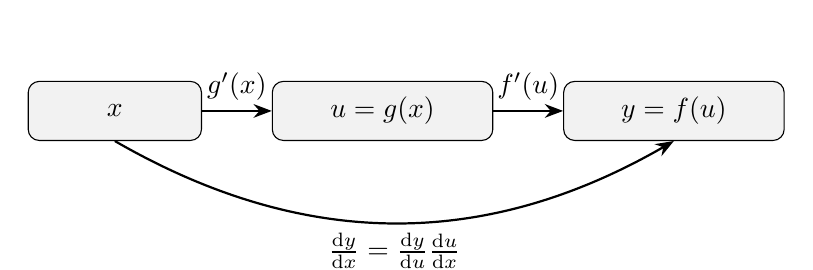
\begin{tikzpicture}[>=Stealth,scale=1.0]
  \node[draw,rounded corners,fill=gray!10,minimum width=2.2cm,minimum height=0.75cm] (x) at (0,0) {$x$};
  \node[draw,rounded corners,fill=gray!10,minimum width=2.8cm,minimum height=0.75cm] (u) at (3.4,0) {$u=g(x)$};
  \node[draw,rounded corners,fill=gray!10,minimum width=2.8cm,minimum height=0.75cm] (y) at (7.1,0) {$y=f(u)$};
  \draw[->,thick] (x) -- node[above] {$g'(x)$} (u);
  \draw[->,thick] (u) -- node[above] {$f'(u)$} (y);
  \draw[->,thick,bend right=30] (x.south) to node[below] {$\frac{\dd y}{\dd x}=\frac{\dd y}{\dd u}\frac{\dd u}{\dd x}$} (y.south);
\end{tikzpicture}
\end{center}

\begin{idea}
链式法则的关键是分清“外层函数”和“内层函数”. 若 $y=f(u)$、$u=g(x)$，则先对外层变量 $u$ 求导，再乘以内层对 $x$ 的导数. 多层复合时逐层相乘.
\end{idea}

\begin{example}[公式求导]
求 $y=(3x^2-1)^5$ 的导数.
\end{example}
\begin{solution}
令 $u=3x^2-1$，$y=u^5$. 由链式法则
\[
y'=5(3x^2-1)^4\cdot6x=30x(3x^2-1)^4.
\]
\end{solution}

\begin{example}[多层复合求导]
求
\[
y=\ee^{\sqrt{x}},\qquad x>0
\]
的导数.
\end{example}
\begin{solution}
这里有两层复合：
\[
x\longmapsto \sqrt{x}\longmapsto \ee^{\sqrt{x}}.
\]
因此
\[
y'=\ee^{\sqrt{x}}\cdot(\sqrt{x})'
=\ee^{\sqrt{x}}\cdot\frac{1}{2\sqrt{x}}
=\frac{\ee^{\sqrt{x}}}{2\sqrt{x}}.
\]
在 $x=0$ 处函数有定义，但上述导数公式不适用；事实上右差商趋于无穷大，因此在通常有限导数意义下不可导.
\end{solution}

\begin{example}[复合与乘积同时出现]
求
\[
y=\ee^{-x}\sin\sqrt{2x},\qquad x>0
\]
的导数.
\end{example}
\begin{solution}
这是两个函数的乘积，其中第二个函数又是复合函数. 由乘积法则，
\[
y'=(-\ee^{-x})\sin\sqrt{2x}
+\ee^{-x}\cdot\frac{\dd}{\dd x}\sin\sqrt{2x}.
\]
对第二项用链式法则：
\[
\frac{\dd}{\dd x}\sin\sqrt{2x}
=\cos\sqrt{2x}\cdot\frac{\dd}{\dd x}(2x)^{1/2}
=\cos\sqrt{2x}\cdot\frac1{\sqrt{2x}}.
\]
故
\[
y'=\ee^{-x}\left(\frac{\cos\sqrt{2x}}{\sqrt{2x}}-\sin\sqrt{2x}\right).
\]
\end{solution}

\begin{example}[对数求导]
求 $y=x^x\ (x>0)$ 的导数.
\end{example}
\begin{solution}
取对数得 $\ln y=x\ln x$. 两边求导：
\[
\frac{y'}{y}=\ln x+1.
\]
因此
\[
y'=x^x(\ln x+1).
\]
\end{solution}
\begin{warning}
$x^x$ 不能直接套用幂函数 $x^a$ 或指数函数 $a^x$ 的公式，因为底数和指数都含 $x$.
\end{warning}

\begin{example}[变底变指数函数]
求
\[
y=(\cot x)^{\cos x}
\]
的导数，其中在所讨论的区间内 $\cot x>0$.
\end{example}
\begin{solution}
由于底数和指数都含 $x$，采用对数求导. 取对数：
\[
\ln y=\cos x\ln(\cot x).
\]
两边对 $x$ 求导：
\[
\frac{y'}{y}
=-\sin x\ln(\cot x)+\cos x\cdot\frac{(\cot x)'}{\cot x}.
\]
又
\[
(\cot x)'=-\csc^2x,\qquad
\frac{(\cot x)'}{\cot x}
=-\frac{\csc^2x}{\cot x}
=-\frac{1}{\sin x\cos x}.
\]
于是
\[
\frac{y'}{y}
=-\sin x\ln(\cot x)-\frac1{\sin x}.
\]
因此
\[
y'=(\cot x)^{\cos x}\left[-\sin x\ln(\cot x)-\frac1{\sin x}\right].
\]
\end{solution}

\begin{example}[对数求导]
设
\[
y=\sqrt{\frac{(x-1)(x-2)}{(x-3)(x-4)}},
\]
其中 $x$ 取在使根式有意义且分母不为零的区间内. 求 $y'$.
\end{example}
\begin{solution}
取对数得
\[
\ln y=\frac12\left[\ln|x-1|+\ln|x-2|-\ln|x-3|-\ln|x-4|\right].
\]
两边求导：
\[
\frac{y'}{y}
=\frac12\left(\frac1{x-1}+\frac1{x-2}-\frac1{x-3}-\frac1{x-4}\right).
\]
因此
\[
y'=\frac12\sqrt{\frac{(x-1)(x-2)}{(x-3)(x-4)}}
\left(\frac1{x-1}+\frac1{x-2}-\frac1{x-3}-\frac1{x-4}\right).
\]
\end{solution}

\begin{proposition}[常用基本导数公式]
在相应定义域内，下列公式成立. 其中 $a>0,\ a\neq1$；对一般实数 $\alpha$，公式 $(x^\alpha)'=\alpha x^{\alpha-1}$ 通常在 $x>0$ 上使用，若 $\alpha$ 为整数或有理数，还需按函数本身的定义域作相应调整.
\[
(C)'=0,\quad (x^\alpha)'=\alpha x^{\alpha-1},\quad (a^x)'=a^x\ln a,\quad (\ee^x)'=\ee^x,
\]
\[
(\log_a |x|)'=\frac1{x\ln a},\quad (\ln |x|)'=\frac1x,
\]
\[
(\sin x)'=\cos x,\quad (\cos x)'=-\sin x,\quad
(\tan x)'=\sec^2x,\quad (\cot x)'=-\csc^2x,
\]
\[
(\sec x)'=\sec x\tan x,\quad (\csc x)'=-\csc x\cot x,
\]
\[
(\arcsin x)'=\frac1{\sqrt{1-x^2}},\quad
(\arccos x)'=-\frac1{\sqrt{1-x^2}},
\]
\[
(\arctan x)'=\frac1{1+x^2},\quad
(\operatorname{arccot}x)'=-\frac1{1+x^2}.
\]
\end{proposition}
\begin{idea}
这些公式是求导计算的基础. 讲授时不宜只背公式：三角函数公式来自导数定义与基本极限，指数与反三角函数公式分别依赖反函数求导和链式法则.
\end{idea}

\subsection{反函数求导与高阶导数}

有些函数本身不是由初等四则运算直接给出，而是作为另一个函数的反函数出现. 例如 $\ln x$ 是 $\ee^x$ 的反函数，$\arcsin x$ 是适当限制定义域后的 $\sin x$ 的反函数. 反函数求导公式说明：若 $y=f(x)$ 可反解为 $x=\varphi(y)$，则反函数图像在对应点的切线斜率等于原函数切线斜率的倒数.

\begin{theorem}[反函数求导公式]
设 $y=f(x)$ 在点 $x_0$ 的某邻域内严格单调、连续，且 $f$ 在 $x_0$ 处可导，$f'(x_0)\neq0$. 设反函数为 $x=\varphi(y)$，$y_0=f(x_0)$. 若 $\varphi$ 在 $y_0$ 处连续，则 $\varphi$ 在 $y_0$ 处可导，且
\[
\varphi'(y_0)=\frac{1}{f'(x_0)}.
\]
\end{theorem}
\begin{proofdetail}
当 $\Delta y\neq0$ 时，由严格单调性知对应的 $\Delta x=\varphi(y_0+\Delta y)-\varphi(y_0)$ 也不为 $0$，并且
\[
\frac{\Delta x}{\Delta y}
=\frac{1}{\frac{f(x_0+\Delta x)-f(x_0)}{\Delta x}}.
\]
由 $\varphi$ 在 $y_0$ 连续，$\Delta y\to0$ 时 $\Delta x\to0$. 因 $f'(x_0)\neq0$，
\[
\lim_{\Delta y\to0}\frac{\Delta x}{\Delta y}
=\frac{1}{\lim_{\Delta x\to0}\frac{f(x_0+\Delta x)-f(x_0)}{\Delta x}}
=\frac1{f'(x_0)}.
\]
故反函数在 $y_0$ 处可导，公式成立.
\end{proofdetail}

\begin{example}[由反函数推出对数函数导数]
由 $y=\log_a x\ (a>0,\ a\neq1,\ x>0)$，推出其导数公式.
\end{example}
\begin{solution}
令 $y=\log_a x$，则 $x=a^y$. 把 $x$ 看成 $y$ 的函数，有
\[
\frac{\dd x}{\dd y}=a^y\ln a=x\ln a.
\]
由反函数求导公式，
\[
\frac{\dd y}{\dd x}
=\frac{1}{\dd x/\dd y}
=\frac{1}{x\ln a}.
\]
当 $a=\ee$ 时得到
\[
(\ln x)'=\frac1x.
\]
\end{solution}

\begin{example}[反三角函数导数]
求 $y=\arcsin x$ 与 $y=\arctan x$ 的导数.
\end{example}
\begin{solution}
若 $y=\arcsin x$，则
\[
x=\sin y,\qquad y\in\left[-\frac{\pi}{2},\frac{\pi}{2}\right].
\]
在 $|x|<1$ 时，$\cos y>0$，故
\[
\frac{\dd x}{\dd y}=\cos y=\sqrt{1-\sin^2y}=\sqrt{1-x^2}.
\]
由反函数求导公式，
\[
(\arcsin x)'=\frac{1}{\sqrt{1-x^2}},\qquad |x|<1.
\]

若 $y=\arctan x$，则 $x=\tan y$，$y\in(-\pi/2,\pi/2)$. 因而
\[
\frac{\dd x}{\dd y}=\sec^2y=1+\tan^2y=1+x^2,
\]
所以
\[
(\arctan x)'=\frac1{1+x^2},\qquad x\in\RR.
\]
\end{solution}

\begin{definition}[高阶导数]
若 $f'$ 在区间上仍可导，则其导数称为 $f$ 的二阶导数，记作 $f''$ 或 $\frac{\dd^2y}{\dd x^2}$. 递推地，$f^{(n)}=(f^{(n-1)})'$ 称为 $n$ 阶导数.
\end{definition}

如果 $s(t)$ 表示直线运动位移，则 $s'(t)$ 是速度，$s''(t)$ 是加速度. 在经济学中，边际函数的导数也有意义：例如 $C''(x)$ 描述边际成本随产量变化的快慢. 因此高阶导数不仅是形式计算，也常用于判断变化趋势、凹凸性和近似公式.

\begin{example}[常用函数高阶导数]
求 $f(x)=\ee^{ax}$ 与 $g(x)=\sin x$ 的 $n$ 阶导数.
\end{example}
\begin{solution}
对指数函数，逐次求导得
\[
f^{(n)}(x)=a^n\ee^{ax}.
\]
对正弦函数，导数每四次循环：
\[
g^{(n)}(x)=\sin\left(x+\frac{n\pi}{2}\right).
\]
可用数学归纳法验证：$n=0$ 成立；若 $g^{(n)}(x)=\sin(x+n\pi/2)$，则
\[
g^{(n+1)}(x)=\cos\left(x+\frac{n\pi}{2}\right)=\sin\left(x+\frac{(n+1)\pi}{2}\right).
\]
\end{solution}

\begin{example}[对数函数的高阶导数]
求 $y=\ln(1+x)$ 的 $n$ 阶导数，其中 $x>-1$.
\end{example}
\begin{solution}
逐次求导：
\[
y'=\frac1{1+x},\qquad
y''=-\frac1{(1+x)^2},\qquad
y'''=\frac{2!}{(1+x)^3}.
\]
由此归纳得到
\[
y^{(n)}=(-1)^{n-1}\frac{(n-1)!}{(1+x)^n},\qquad n=1,2,3,\ldots.
\]
验证如下. 当 $n=1$ 时公式成立. 若
\[
y^{(n)}=(-1)^{n-1}(n-1)!(1+x)^{-n},
\]
则
\[
y^{(n+1)}
=(-1)^{n-1}(n-1)![-n(1+x)^{-n-1}]
=(-1)^n\frac{n!}{(1+x)^{n+1}}.
\]
故公式对所有正整数 $n$ 成立.
\end{solution}

\begin{example}[验证二阶导数关系]
设 $y=\ee^x\sin x$，证明
\[
y''-2y'+2y=0.
\]
\end{example}
\begin{solution}
先求一阶导数：
\[
y'=\ee^x\sin x+\ee^x\cos x=\ee^x(\sin x+\cos x).
\]
再求二阶导数：
\[
y''=\ee^x(\sin x+\cos x)+\ee^x(\cos x-\sin x)=2\ee^x\cos x.
\]
因此
\[
y''-2y'+2y
=2\ee^x\cos x-2\ee^x(\sin x+\cos x)+2\ee^x\sin x=0.
\]
等式成立.
\end{solution}

\begin{example}[Leibniz 公式]
求 $y=x^2\ee^x$ 的 $n$ 阶导数.
\end{example}
\begin{solution}
Leibniz 公式为
\[
(uv)^{(n)}=\sum_{k=0}^n\binom nk u^{(k)}v^{(n-k)}.
\]
取 $u=x^2,\ v=\ee^x$. 当 $k\geq3$ 时 $u^{(k)}=0$，故
\[
y^{(n)}=\binom n0x^2\ee^x+\binom n1(2x)\ee^x+\binom n2(2)\ee^x
=\ee^x\left[x^2+2nx+n(n-1)\right].
\]
\end{solution}

\begin{theorem}[Leibniz 公式]
若 $u,v$ 均有 $n$ 阶导数，则
\[
(uv)^{(n)}=\sum_{k=0}^{n}\binom{n}{k}u^{(k)}v^{(n-k)}.
\]
\end{theorem}
\begin{proofdetail}
用数学归纳法. 当 $n=1$ 时即乘法求导法则. 假设公式对 $n$ 成立，则
\[
(uv)^{(n+1)}
=\frac{\dd}{\dd x}\sum_{k=0}^{n}\binom{n}{k}u^{(k)}v^{(n-k)}
\]
\[
=\sum_{k=0}^{n}\binom{n}{k}u^{(k+1)}v^{(n-k)}
+\sum_{k=0}^{n}\binom{n}{k}u^{(k)}v^{(n-k+1)}.
\]
第一和中令 $j=k+1$，得
\[
\sum_{j=1}^{n+1}\binom{n}{j-1}u^{(j)}v^{(n+1-j)}
+\sum_{j=0}^{n}\binom{n}{j}u^{(j)}v^{(n+1-j)}.
\]
合并同类项，端点系数为 $1$，中间项系数为
\[
\binom{n}{j-1}+\binom{n}{j}=\binom{n+1}{j}.
\]
于是
\[
(uv)^{(n+1)}=\sum_{j=0}^{n+1}\binom{n+1}{j}u^{(j)}v^{(n+1-j)}.
\]
归纳完成.
\end{proofdetail}

\subsection{隐函数求导与参数方程求导}

前面讨论的函数大多写成 $y=f(x)$，这种形式称为显函数. 但在实际问题和几何问题中，变量之间常由方程给出，例如
\[
x^2+y^2=1,\qquad x^2+xy+y^2=3.
\]
它们未必能方便地解出 $y=f(x)$. 由方程 $F(x,y)=0$ 在某个范围内确定的函数称为隐函数. 例如
\[
\sqrt{y}+x^2-1=0
\]
在满足 $1-x^2\geq0$ 且 $\sqrt{y}=1-x^2$ 的范围内可写成
\[
y=(1-x^2)^2.
\]
但并不是每个方程都在任意点附近确定唯一函数. 本讲义在求导时默认题目所给方程已经在所讨论点附近确定了可导函数；更一般的存在唯一性条件将在多元函数课程中进一步解释.

\begin{center}
\begin{tikzpicture}[scale=1.15,>=Stealth]
  \draw[->] (-1.9,0) -- (1.9,0) node[right] {$x$};
  \draw[->] (0,-1.55) -- (0,1.55) node[above] {$y$};
  \draw[thick,domain=0:360,samples=160] plot ({cos(\x)},{sin(\x)});
  \fill (0.6,0.8) circle (1.5pt) node[above right] {$P(x,y)$};
  \draw[dashed] (0.6,0) -- (0.6,0.8) -- (0,0.8);
  \node at (0,-1.85) {$x^2+y^2=1$ 给出的曲线可在局部看作 $y=y(x)$};
\end{tikzpicture}
\end{center}

\begin{proposition}[隐函数一阶求导]
若方程 $F(x,y)=0$ 在某区间上确定可导函数 $y=y(x)$，且 $F$ 有连续偏导数、$F_y(x,y)\neq0$，则
\[
y'=-\frac{F_x}{F_y},
\]
其中右端在 $(x,y(x))$ 处取值.
\end{proposition}
\begin{proofdetail}
由恒等式 $F(x,y(x))\equiv0$ 对 $x$ 求导. 复合函数求导给出
\[
F_x(x,y(x))+F_y(x,y(x))y'(x)=0.
\]
由于 $F_y(x,y(x))\neq0$，移项并相除得到公式.
\end{proofdetail}

\begin{example}[隐函数一阶导数]
由方程 $x^2+xy+y^2=3$ 确定 $y=y(x)$，求 $y'$.
\end{example}
\begin{solution}
两边对 $x$ 求导：
\[
2x+y+xy'+2yy'=0.
\]
整理得
\[
y'=-\frac{2x+y}{x+2y}.
\]
该公式在 $x+2y\neq0$ 的点成立.
\end{solution}

\begin{example}[先说明隐函数再求导]
设方程
\[
\sqrt{y}+x^2-1=0
\]
在 $|x|<1$ 附近确定函数 $y=y(x)$. 用两种方法求 $y'$.
\end{example}
\begin{solution}
方法一：先解出显函数. 由方程得
\[
\sqrt{y}=1-x^2.
\]
当 $|x|<1$ 时右端为正，故
\[
y=(1-x^2)^2.
\]
于是
\[
y'=2(1-x^2)(-2x)=-4x(1-x^2).
\]

方法二：直接对原方程求导. 注意
\[
\frac{\dd}{\dd x}\sqrt{y}
=\frac{1}{2\sqrt{y}}y',
\]
因此
\[
\frac{y'}{2\sqrt{y}}+2x=0,
\qquad
y'=-4x\sqrt{y}.
\]
再代入 $\sqrt{y}=1-x^2$，得
\[
y'=-4x(1-x^2).
\]
两种方法结果一致.
\end{solution}

\begin{example}[隐函数二阶导数]
设 $x^2+y^2=1$ 在点附近确定 $y=y(x)$，求 $y''$.
\end{example}
\begin{solution}
一阶求导得
\[
2x+2yy'=0,\qquad y'=-\frac{x}{y}\quad(y\neq0).
\]
对 $2x+2yy'=0$ 再求导：
\[
2+2(y')^2+2yy''=0.
\]
故
\[
y''=-\frac{1+(y')^2}{y}=-\frac{1+x^2/y^2}{y}
=-\frac{x^2+y^2}{y^3}=-\frac1{y^3}.
\]
\end{solution}

\begin{example}[隐函数切线]
求曲线
\[
xy-\ee^x+\ee^y=0
\]
在点 $(0,0)$ 处的切线方程.
\end{example}
\begin{solution}
把 $y$ 看成 $x$ 的函数，对方程两边求导，得
\[
y+xy'-\ee^x+\ee^y y'=0.
\]
整理得
\[
(x+\ee^y)y'=\ee^x-y,\qquad
y'=\frac{\ee^x-y}{x+\ee^y}.
\]
在 $(0,0)$ 处，
\[
y'(0)=\frac{1-0}{0+1}=1.
\]
因此切线方程为 $y=x$.
\end{solution}

\begin{proposition}[参数方程求导]
若曲线由 $x=\varphi(t),\,y=\psi(t)$ 给出，且 $\varphi'(t)\neq0$，则
\[
\frac{\dd y}{\dd x}=\frac{\psi'(t)}{\varphi'(t)}.
\]
若还存在二阶导数，则
\[
\frac{\dd^2y}{\dd x^2}
=\frac{1}{\varphi'(t)}\frac{\dd}{\dd t}\left(\frac{\psi'(t)}{\varphi'(t)}\right).
\]
\end{proposition}
\begin{proofdetail}
当 $\varphi'(t)\neq0$ 时，局部可把 $t$ 看成 $x$ 的函数. 由链式法则，
\[
\frac{\dd y}{\dd t}=\frac{\dd y}{\dd x}\frac{\dd x}{\dd t}.
\]
两边除以 $\dd x/\dd t=\varphi'(t)$ 得第一式. 对第一式再关于 $x$ 求导，而 $\frac{\dd}{\dd x}=\frac1{\varphi'(t)}\frac{\dd}{\dd t}$，得第二式.
\end{proofdetail}

\begin{example}[参数方程求切线]
曲线由
\[
x=t^2,\qquad y=t^3
\]
给出. 求 $t=1$ 处的切线方程.
\end{example}
\begin{solution}
当 $t=1$ 时，曲线上的点为 $(1,1)$. 又
\[
\frac{\dd y}{\dd x}
=\frac{\dd y/\dd t}{\dd x/\dd t}
=\frac{3t^2}{2t}
=\frac{3t}{2}\qquad(t\neq0).
\]
在 $t=1$ 处斜率为 $3/2$，故切线方程为
\[
y-1=\frac32(x-1).
\]
\end{solution}

\begin{example}[增长率]
某种药物在血液中的浓度 $C$ 与时间 $t$ 的关系为 $C(t)=te^{-0.5t}$，求浓度变化率，并判断 $t=2$ 时浓度是增加还是减少.
\end{example}
\begin{solution}
\[
C'(t)=e^{-0.5t}-0.5te^{-0.5t}=e^{-0.5t}(1-0.5t).
\]
当 $t=2$ 时，$C'(2)=0$，说明此刻浓度达到由增转减的临界状态；仅从瞬时变化率看，此刻既不增加也不减少.
\end{solution}

\begin{example}[边际成本变化率]
某产品总成本函数为
\[
C(x)=0.02x^2+6x+300,\qquad x\geq0.
\]
求边际成本和边际成本的变化率，并解释 $C''(x)$ 的含义.
\end{example}
\begin{solution}
边际成本是总成本对产量的导数：
\[
C'(x)=0.04x+6.
\]
边际成本的变化率为
\[
C''(x)=0.04.
\]
这说明产量每增加一个单位，边际成本按近似 $0.04$ 的速度增加. 这里 $C'(x)$ 表示“在产量为 $x$ 附近多生产一个单位所增加的成本”，而 $C''(x)$ 描述这个边际成本本身随产量增加而上升的快慢.
\end{solution}

\subsection{课后习题}
\begin{enumerate}[label=\textbf{练习\arabic*.},leftmargin=2.2em]
\item 求下列函数的导数：
\[
y=3x^2+4\ln x-5\cos x,\qquad
y=\ln(\sin x),\qquad
y=\ee^{\sqrt{x}}.
\]
\item 求
\[
y=\frac{x^2\sin x}{1+x^2}
\]
的导数，并说明用到了哪些求导法则.
\item 求下列函数的导数：
\[
y=(1+x^2)^{\arctan x},\qquad
y=(\cot x)^{\cos x}.
\]
\item 由反函数求导公式推出 $y=\arccos x$ 的导数.
\item 求 $y=x^2\ln x$ 的二阶导数，其中 $x>0$.
\item 求 $y=x^2\ee^x$ 的 $n$ 阶导数.
\item 设 $x^3+y^3-3xy=0$ 确定 $y=y(x)$，求 $y'$.
\item 求曲线
\[
xy+\ln y=1
\]
在点 $(1,1)$ 处的切线方程.
\item 曲线由参数方程
\[
x=t-\sin t,\qquad y=1-\cos t
\]
给出，求 $\frac{\dd y}{\dd x}$.
\item 某产品总收入函数为
\[
R(x)=50x-0.1x^2.
\]
求边际收入函数和边际收入的变化率，并解释 $R''(x)$ 的经济含义.
\end{enumerate}

\subsection{参考解答}
\begin{enumerate}[label=\textbf{练习\arabic*.},leftmargin=2.2em]
\item
\[
(3x^2+4\ln x-5\cos x)'=6x+\frac4x+5\sin x.
\]
又
\[
(\ln\sin x)'=\frac{\cos x}{\sin x}=\cot x,
\]
其中需 $\sin x>0$ 或至少在选定区间内 $\ln(\sin x)$ 有定义. 最后
\[
(\ee^{\sqrt{x}})'=\ee^{\sqrt{x}}\cdot\frac1{2\sqrt{x}}
=\frac{\ee^{\sqrt{x}}}{2\sqrt{x}},\qquad x>0.
\]
\item 先对分子用乘积法则，再对整体用商法：
\[
\left(x^2\sin x\right)'=2x\sin x+x^2\cos x,
\]
\[
y'=\frac{(2x\sin x+x^2\cos x)(1+x^2)-2x\cdot x^2\sin x}{(1+x^2)^2}.
\]
化简得
\[
y'=\frac{2x\sin x+x^2\cos x+x^4\cos x}{(1+x^2)^2}.
\]
\item 对第一个函数取对数：
\[
\ln y=(\arctan x)\ln(1+x^2),
\]
故
\[
y'=(1+x^2)^{\arctan x}\left[\frac{\ln(1+x^2)}{1+x^2}+\frac{2x\arctan x}{1+x^2}\right].
\]
对第二个函数，取对数得
\[
\ln y=\cos x\ln(\cot x).
\]
因此
\[
y'=(\cot x)^{\cos x}\left[-\sin x\ln(\cot x)-\frac1{\sin x}\right],
\]
其中要求在所讨论区间内 $\cot x>0$.
\item 令 $y=\arccos x$，则 $x=\cos y$，$y\in[0,\pi]$. 当 $-1<x<1$ 时，$\sin y>0$，故
\[
\frac{\dd x}{\dd y}=-\sin y=-\sqrt{1-x^2}.
\]
由反函数求导公式，
\[
(\arccos x)'=-\frac1{\sqrt{1-x^2}},\qquad -1<x<1.
\]
\item
\[
y'=2x\ln x+x,\qquad y''=2\ln x+3.
\]
\item 由 Leibniz 公式，取 $u=x^2,\ v=\ee^x$. 因 $u^{(k)}=0\ (k\geq3)$，得
\[
y^{(n)}=\ee^x\left[x^2+2nx+n(n-1)\right].
\]
\item 两边对 $x$ 求导：
\[
3x^2+3y^2y'-3y-3xy'=0,
\]
故
\[
y'=\frac{y-x^2}{y^2-x}.
\]
\item 将 $y$ 看成 $x$ 的函数. 对
\[
xy+\ln y=1
\]
两边求导：
\[
y+xy'+\frac{y'}{y}=0.
\]
在 $(1,1)$ 处，
\[
1+y'+y'=0,\qquad y'=-\frac12.
\]
故切线方程为
\[
y-1=-\frac12(x-1).
\]
\item
\[
\frac{\dd y}{\dd x}=\frac{\sin t}{1-\cos t},
\]
其中 $1-\cos t\neq0$.
\item
\[
R'(x)=50-0.2x,\qquad R''(x)=-0.2.
\]
其中 $R'(x)$ 为边际收入，表示销量在 $x$ 附近增加一个单位时收入的近似增量；$R''(x)=-0.2$ 表示边际收入随销量增加而下降，且下降速度为常数 $0.2$.
\end{enumerate}

\section{微分与多元函数微分}
\renewEnvironmentCounter
\subsection{一元函数的微分与线性近似}

前两章中，导数描述的是函数在一点的瞬时变化率. 微分进一步强调另一件事：在自变量改变量很小时，函数增量的主要部分是一个线性函数. 这正是“用直线近似曲线”“用切平面近似曲面”的数学基础.

以正方形面积为例. 设边长为 $x$，面积为 $S=x^2$. 当边长由 $x$ 增加到 $x+\Delta x$，其中图中取 $\Delta x>0$，面积增量为
\[
\Delta S=(x+\Delta x)^2-x^2=2x\Delta x+(\Delta x)^2.
\]
这里 $2x\Delta x$ 是关于 $\Delta x$ 的线性主部，$(\Delta x)^2$ 是比 $\Delta x$ 高阶的误差项. 因而当 $|\Delta x|$ 很小时，
\[
\Delta S\approx 2x\Delta x.
\]

\begin{center}
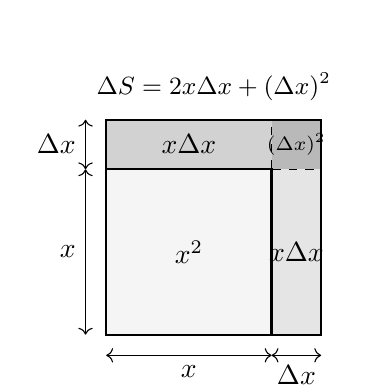
\begin{tikzpicture}[scale=1.05]
  \fill[gray!8] (0,0) rectangle (2,2);
  \fill[gray!20] (2,0) rectangle (2.6,2);
  \fill[gray!35] (0,2) rectangle (2,2.6);
  \fill[gray!55] (2,2) rectangle (2.6,2.6);
  \draw[thick] (0,0) rectangle (2,2);
  \draw[thick] (0,0) rectangle (2.6,2.6);
  \draw[dashed] (2,0)--(2,2.6);
  \draw[dashed] (0,2)--(2.6,2);
  \draw[<->] (0,-0.25)--(2,-0.25) node[midway,below] {$x$};
  \draw[<->] (2,-0.25)--(2.6,-0.25) node[midway,below] {$\Delta x$};
  \draw[<->] (-0.25,0)--(-0.25,2) node[midway,left] {$x$};
  \draw[<->] (-0.25,2)--(-0.25,2.6) node[midway,left] {$\Delta x$};
  \node at (1,1) {$x^2$};
  \node at (2.3,1) {$x\Delta x$};
  \node at (1,2.3) {$x\Delta x$};
  \node at (2.3,2.3) {\scriptsize $(\Delta x)^2$};
  \node at (1.3,3.0) {\small $\Delta S=2x\Delta x+(\Delta x)^2$};
\end{tikzpicture}
\end{center}

\begin{definition}[一元函数可微与微分]
设函数 $y=f(x)$ 在 $x$ 附近有定义. 当自变量增量为 $\Delta x$ 时，函数增量为
\[
\Delta y=f(x+\Delta x)-f(x).
\]
若存在与 $\Delta x$ 无关的常数 $A$，使得
\[
\Delta y=A\Delta x+o(\Delta x)\qquad(\Delta x\to0),
\]
则称 $f$ 在 $x$ 处可微，并称线性主部 $A\Delta x$ 为 $f$ 在 $x$ 处的微分，记作
\[
\dd y=A\Delta x.
\]
通常记 $\dd x=\Delta x$，于是微分写成 $\dd y=A\dd x$.
\end{definition}

\begin{theorem}[一元可导与可微等价]
$f$ 在 $x$ 处可微，当且仅当 $f$ 在 $x$ 处可导. 此时
\[
A=f'(x),\qquad \dd y=f'(x)\dd x.
\]
\end{theorem}
\begin{proofdetail}
若 $f$ 在 $x$ 处可微，则
\[
f(x+\Delta x)-f(x)=A\Delta x+o(\Delta x).
\]
当 $\Delta x\neq0$ 时，两边除以 $\Delta x$，得
\[
\frac{f(x+\Delta x)-f(x)}{\Delta x}
=A+\frac{o(\Delta x)}{\Delta x}.
\]
由 $o(\Delta x)$ 的定义，
\[
\frac{o(\Delta x)}{\Delta x}\to0\qquad(\Delta x\to0),
\]
所以导数存在，且 $f'(x)=A$.

反过来，若 $f$ 在 $x$ 处可导，则
\[
\frac{f(x+\Delta x)-f(x)}{\Delta x}\to f'(x).
\]
定义
\[
\alpha(\Delta x)=
\begin{cases}
\dfrac{f(x+\Delta x)-f(x)}{\Delta x}-f'(x),&\Delta x\neq0,\\[0.8em]
0,&\Delta x=0.
\end{cases}
\]
则 $\alpha(\Delta x)\to0$，并且
\[
\Delta y=f'(x)\Delta x+\alpha(\Delta x)\Delta x
=f'(x)\Delta x+o(\Delta x).
\]
因此 $f$ 在 $x$ 处可微，且 $\dd y=f'(x)\dd x$.
\end{proofdetail}

\begin{proposition}[微分运算法则]
若 $u=u(x),v=v(x)$ 在 $x$ 处可微，$c$ 为常数，则
\[
\dd(cu)=c\,\dd u,\qquad \dd(u+v)=\dd u+\dd v,
\]
\[
\dd(uv)=u\,\dd v+v\,\dd u,
\]
若 $v\neq0$，则
\[
\dd\left(\frac{u}{v}\right)=\frac{v\,\dd u-u\,\dd v}{v^2}.
\]
若 $y=f(u)$，$u=g(x)$，且相应函数可微，则
\[
\dd y=f'(u)\dd u.
\]
\end{proposition}
\begin{proofdetail}
由一元可导与可微等价，$u,v$ 可微等价于可导. 前四个公式分别由常数倍、和、积、商的求导法则乘以 $\dd x$ 得到. 例如
\[
\dd(uv)=(uv)'\dd x=(u'v+uv')\dd x=v(u'\dd x)+u(v'\dd x)=v\,\dd u+u\,\dd v.
\]
复合情形中，链式法则给出
\[
\dd y=\frac{\dd y}{\dd x}\dd x=f'(u)g'(x)\dd x=f'(u)\dd u.
\]
这说明无论 $u$ 是自变量还是 $x$ 的函数，微分形式 $\dd y=f'(u)\dd u$ 保持不变.
\end{proofdetail}

\begin{proposition}[微分的几何意义]
若 $f$ 在 $x_0$ 处可导，则曲线 $y=f(x)$ 在点 $M=(x_0,f(x_0))$ 附近可用切线作局部近似：
\[
f(x_0+\Delta x)-f(x_0)=f'(x_0)\Delta x+o(\Delta x).
\]
其中 $\Delta y=f(x_0+\Delta x)-f(x_0)$ 是真实增量，$\dd y=f'(x_0)\Delta x$ 是切线给出的线性近似，二者差为高阶误差.
\end{proposition}

\begin{center}
\begin{tikzpicture}[scale=1.0,>=Stealth]
  \draw[->] (-0.2,0)--(6.4,0) node[right] {$x$};
  \draw[->] (0,0.35)--(0,3.1) node[above] {$y$};
  \draw[domain=0.55:4.9,smooth,variable=\x,thick] plot ({\x},{0.16*(\x-1)*(\x-1)+1});
  \coordinate (M) at (2,1.16);
  \coordinate (T) at (3.4,1.608);
  \coordinate (N) at (3.4,1.922);
  \coordinate (B) at (3.4,1.16);
  \draw[thick] (0.7,0.744)--(5.15,2.168);
  \draw[dashed] (M)--(2,0) node[below] {$x_0$};
  \draw[dashed] (N)--(3.4,0) node[below] {$x_0+\Delta x$};
  \draw[dashed] (M)--(B);
  \draw[dashed] (N)--(T);
  \draw[dashed] (T)--(B);
  \draw[<->] (2,0.55)--(3.4,0.55) node[midway,below] {$\Delta x$};
  \draw[<->] (3.66,1.16)--(3.66,1.608);
  \draw[<->] (3.66,1.608)--(3.66,1.922);
  \draw[thin] (3.66,1.384)--(4.65,1.34) node[right] {$\dd y$};
  \draw[thin] (3.66,1.765)--(4.65,1.78) node[right] {\scriptsize $\Delta y-\dd y$};
  \fill (M) circle (1.5pt) node[above left] {$M$};
  \fill (T) circle (1.4pt) node[below left] {$T$};
  \fill (N) circle (1.5pt) node[above left] {$N$};
  \node[fill=white,inner sep=1pt] at (4.95,2.35) {切线};
\end{tikzpicture}
\end{center}

\begin{example}[近似计算]
用微分近似计算 $\sqrt{4.04}$.
\end{example}
\begin{solution}
取 $f(x)=\sqrt{x}$，在 $x=4$ 处线性化. 有
\[
f(4)=2,\qquad f'(x)=\frac{1}{2\sqrt{x}},\qquad f'(4)=\frac14.
\]
当 $\Delta x=0.04$ 时，
\[
\sqrt{4.04}=f(4+0.04)\approx f(4)+f'(4)\Delta x
=2+\frac14\cdot0.04=2.01.
\]
\end{solution}
\begin{warning}
微分近似不是等式. 本题真实值约为 $2.009975\cdots$，近似值 $2.01$ 的误差很小，是因为 $\Delta x=0.04$ 相对基点 $4$ 很小.
\end{warning}

\begin{example}[相对误差]
球的半径 $r$ 测量有小误差 $\Delta r$. 设体积 $V=\frac43\pi r^3$. 用微分估计体积的相对误差.
\end{example}
\begin{solution}
体积微分为
\[
\dd V=4\pi r^2\dd r.
\]
当 $\Delta r$ 很小时，$\Delta V\approx \dd V=4\pi r^2\Delta r$. 因此体积相对误差近似为
\[
\frac{\Delta V}{V}\approx
\frac{\dd V}{V}
=\frac{4\pi r^2\dd r}{\frac43\pi r^3}
=3\frac{\dd r}{r}.
\]
这说明半径的相对误差约放大为体积相对误差的三倍. 该结论来自数学模型 $V=\frac43\pi r^3$，不依赖具体计量单位.
\end{solution}

\begin{example}[微分形式不变性]
求函数
\[
y=\ee^{1-3x}\sin2x
\]
的微分.
\end{example}
\begin{solution}
由乘积微分法则，
\[
\dd y=\sin2x\,\dd(\ee^{1-3x})+\ee^{1-3x}\,\dd(\sin2x).
\]
利用微分形式不变性，
\[
\dd(\ee^{1-3x})=\ee^{1-3x}\dd(1-3x)=-3\ee^{1-3x}\dd x,
\]
\[
\dd(\sin2x)=\cos2x\,\dd(2x)=2\cos2x\,\dd x.
\]
故
\[
\dd y=\ee^{1-3x}(2\cos2x-3\sin2x)\dd x.
\]
\end{solution}

\subsection{偏导数与高阶偏导数}

二元函数 $z=f(x,y)$ 的输入是平面上的点. 若只让 $x$ 改变而保持 $y$ 不变，就得到沿平行于 $x$ 轴方向的变化率；若只让 $y$ 改变而保持 $x$ 不变，就得到沿平行于 $y$ 轴方向的变化率. 这两个变化率分别称为偏导数.

\begin{definition}[偏导数]
设 $z=f(x,y)$ 在点 $(x_0,y_0)$ 的某邻域内有定义. 若极限
\[
\lim_{h\to0}\frac{f(x_0+h,y_0)-f(x_0,y_0)}{h}
\]
存在，则称其为 $f$ 对 $x$ 的偏导数，记为
\[
f_x(x_0,y_0),\qquad \frac{\partial f}{\partial x}(x_0,y_0).
\]
若极限
\[
\lim_{k\to0}\frac{f(x_0,y_0+k)-f(x_0,y_0)}{k}
\]
存在，则称其为 $f$ 对 $y$ 的偏导数，记为 $f_y(x_0,y_0)$ 或 $\frac{\partial f}{\partial y}(x_0,y_0)$.
\end{definition}

\begin{example}[偏导计算]
设 $f(x,y)=x^2y+\sin(xy)$，求 $f_x,f_y$.
\end{example}
\begin{solution}
求 $f_x$ 时把 $y$ 看作常数：
\[
f_x=2xy+y\cos(xy).
\]
求 $f_y$ 时把 $x$ 看作常数：
\[
f_y=x^2+x\cos(xy).
\]
偏导计算中的“把另一个变量看作常数”不是说另一个变量永远不变，而是说此刻只沿一个坐标方向取变化率.
\end{solution}

\begin{example}[边际产量]
设 Cobb-Douglas 型生产函数为
\[
Q(K,L)=A K^\alpha L^\beta,\qquad A>0,\quad K>0,\quad L>0.
\]
其中 $K$ 表示资本投入，$L$ 表示劳动投入，$Q$ 表示产出. 求资本的边际产量和劳动的边际产量.
\end{example}
\begin{solution}
资本的边际产量指在劳动投入 $L$ 固定时，产出对资本投入 $K$ 的偏导数：
\[
Q_K=A\alpha K^{\alpha-1}L^\beta.
\]
劳动的边际产量指在资本投入 $K$ 固定时，产出对劳动投入 $L$ 的偏导数：
\[
Q_L=A\beta K^\alpha L^{\beta-1}.
\]
这两个量分别表示在当前投入水平附近，单独增加一单位资本或一单位劳动时，产出的近似增量.
\end{solution}

\begin{definition}[二阶偏导数]
若一阶偏导函数 $f_x,f_y$ 仍有偏导数，则称这些偏导数为二阶偏导数，记作
\[
f_{xx}=\frac{\partial^2 f}{\partial x^2},\qquad
f_{xy}=\frac{\partial^2 f}{\partial y\partial x},
\]
\[
f_{yx}=\frac{\partial^2 f}{\partial x\partial y},\qquad
f_{yy}=\frac{\partial^2 f}{\partial y^2}.
\]
这里 $f_{xy}$ 表示先对 $x$ 求偏导，再对 $y$ 求偏导；$f_{yx}$ 表示先对 $y$ 求偏导，再对 $x$ 求偏导.
\end{definition}

\begin{theorem}[混合偏导相等的充分条件]
若 $f_{xy}$ 与 $f_{yx}$ 在点 $(x_0,y_0)$ 的某邻域内存在，并且都在 $(x_0,y_0)$ 连续，则
\[
f_{xy}(x_0,y_0)=f_{yx}(x_0,y_0).
\]
\end{theorem}
\begin{proofdetail}
取充分小的非零 $h,k$，记
\[
\Delta=f(x_0+h,y_0+k)-f(x_0+h,y_0)-f(x_0,y_0+k)+f(x_0,y_0).
\]
先把 $\Delta$ 写为
\[
\Delta=\bigl[f(x_0+h,y_0+k)-f(x_0,y_0+k)\bigr]
-\bigl[f(x_0+h,y_0)-f(x_0,y_0)\bigr].
\]
对函数
\[
\Phi(y)=f(x_0+h,y)-f(x_0,y)
\]
在区间端点 $y_0,y_0+k$ 使用一元中值定理，存在 $\eta$ 介于 $0$ 与 $k$ 之间，使
\[
\Delta=\Phi'(y_0+\eta)k
=\bigl[f_y(x_0+h,y_0+\eta)-f_y(x_0,y_0+\eta)\bigr]k.
\]
再对函数 $x\mapsto f_y(x,y_0+\eta)$ 在 $x_0,x_0+h$ 上使用中值定理，存在 $\xi$ 介于 $0$ 与 $h$ 之间，使
\[
\Delta=f_{yx}(x_0+\xi,y_0+\eta)hk.
\]
因此
\[
\frac{\Delta}{hk}=f_{yx}(x_0+\xi,y_0+\eta).
\]

另一方面，把 $\Delta$ 写为
\[
\Delta=\bigl[f(x_0+h,y_0+k)-f(x_0+h,y_0)\bigr]
-\bigl[f(x_0,y_0+k)-f(x_0,y_0)\bigr],
\]
同理可得存在 $\xi_1$ 介于 $0$ 与 $h$ 之间、$\eta_1$ 介于 $0$ 与 $k$ 之间，使
\[
\frac{\Delta}{hk}=f_{xy}(x_0+\xi_1,y_0+\eta_1).
\]
令 $(h,k)\to(0,0)$，由 $f_{xy},f_{yx}$ 在 $(x_0,y_0)$ 连续，两种表示的极限分别为 $f_{xy}(x_0,y_0)$ 与 $f_{yx}(x_0,y_0)$，而左端是同一个量的极限，故两者相等.
\end{proofdetail}

\begin{example}[二阶偏导]
设 $f(x,y)=x^3y^2+\ee^{xy}$，求 $f_{xy}$ 与 $f_{yx}$.
\end{example}
\begin{solution}
先求
\[
f_x=3x^2y^2+y\ee^{xy},
\]
再对 $y$ 求偏导：
\[
f_{xy}=6x^2y+\ee^{xy}+xy\ee^{xy}.
\]
另一方面，
\[
f_y=2x^3y+x\ee^{xy},
\]
再对 $x$ 求偏导：
\[
f_{yx}=6x^2y+\ee^{xy}+xy\ee^{xy}.
\]
两者相等. 这里函数由初等函数复合而成，各相关偏导连续，因此符合混合偏导相等的充分条件.
\end{solution}

\begin{example}[偏导存在不推出连续]
设
\[
f(x,y)=
\begin{cases}
\dfrac{xy}{x^2+y^2},&(x,y)\neq(0,0),\\[0.6em]
0,&(x,y)=(0,0).
\end{cases}
\]
证明 $f_x(0,0),f_y(0,0)$ 存在，但 $f$ 在 $(0,0)$ 不连续.
\end{example}
\begin{solution}
按定义，
\[
f_x(0,0)=\lim_{h\to0}\frac{f(h,0)-f(0,0)}{h}=0,\qquad
f_y(0,0)=\lim_{h\to0}\frac{f(0,h)-f(0,0)}{h}=0.
\]
但沿直线 $y=x$，
\[
f(x,x)=\frac{x^2}{2x^2}=\frac12\quad(x\neq0),
\]
故 $\lim_{(x,y)\to(0,0)}f(x,y)$ 不等于 $0$，函数在原点不连续.
\end{solution}
\begin{warning}
偏导数只检测坐标轴方向的变化，不能控制所有趋近方向. 因此“两个偏导数都存在”远弱于“一元函数可导”.
\end{warning}

\subsection{全微分与多元链式法则}

二元函数的偏导数只给出两个坐标方向的变化率. 若要像一元函数那样用一个线性表达式近似总增量，就需要全微分. 全微分的线性主部同时包含 $\Delta x$ 与 $\Delta y$：
\[
\Delta z\approx f_x(x_0,y_0)\Delta x+f_y(x_0,y_0)\Delta y.
\]

\begin{definition}[二元函数可微与全微分]
设 $z=f(x,y)$ 在 $(x_0,y_0)$ 附近有定义. 若
\[
\Delta z=f(x_0+\Delta x,y_0+\Delta y)-f(x_0,y_0)
\]
可写成
\[
\Delta z=A\Delta x+B\Delta y+o(\rho),
\qquad \rho=\sqrt{(\Delta x)^2+(\Delta y)^2},
\]
则称 $f$ 在 $(x_0,y_0)$ 可微，并称
\[
\dd z=A\dd x+B\dd y
\]
为 $f$ 在该点的全微分.
\end{definition}

\begin{theorem}[可微推出连续且偏导存在]
若 $f$ 在 $(x_0,y_0)$ 可微，则 $f$ 在该点连续，且 $f_x(x_0,y_0),f_y(x_0,y_0)$ 存在，并且
\[
\dd z=f_x(x_0,y_0)\dd x+f_y(x_0,y_0)\dd y.
\]
\end{theorem}
\begin{proofdetail}
由可微性，
\[
\Delta z=A\Delta x+B\Delta y+o(\rho).
\]
由于 $|\Delta x|\leq\rho,\ |\Delta y|\leq\rho$，当 $\rho\to0$ 时，
\[
A\Delta x+B\Delta y\to0,\qquad o(\rho)\to0.
\]
故 $\Delta z\to0$，即 $f$ 在 $(x_0,y_0)$ 连续.

取 $\Delta y=0$，则 $\rho=|\Delta x|$，且
\[
f(x_0+\Delta x,y_0)-f(x_0,y_0)=A\Delta x+o(|\Delta x|).
\]
当 $\Delta x\neq0$ 时除以 $\Delta x$ 并令 $\Delta x\to0$，得
\[
f_x(x_0,y_0)=A.
\]
同理取 $\Delta x=0$ 得 $f_y(x_0,y_0)=B$. 因此
\[
\dd z=f_x(x_0,y_0)\dd x+f_y(x_0,y_0)\dd y.
\]
\end{proofdetail}

\begin{theorem}[偏导连续推出可微]
若 $f_x,f_y$ 在 $(x_0,y_0)$ 的某邻域内存在，并且在 $(x_0,y_0)$ 连续，则 $f$ 在 $(x_0,y_0)$ 可微.
\end{theorem}
\begin{proofdetail}
记
\[
\Delta z=f(x_0+\Delta x,y_0+\Delta y)-f(x_0,y_0).
\]
分两段改变变量：
\[
\Delta z=[f(x_0+\Delta x,y_0+\Delta y)-f(x_0,y_0+\Delta y)]
+[f(x_0,y_0+\Delta y)-f(x_0,y_0)].
\]
对第一项把 $y_0+\Delta y$ 固定，对一元函数 $x\mapsto f(x,y_0+\Delta y)$ 使用中值定理. 当 $\Delta x\neq0$ 时，存在 $\theta_1\in(0,1)$ 使
\[
f(x_0+\Delta x,y_0+\Delta y)-f(x_0,y_0+\Delta y)
=f_x(x_0+\theta_1\Delta x,y_0+\Delta y)\Delta x.
\]
当 $\Delta x=0$ 时该等式也成立，因为两边均为 $0$，$\theta_1$ 可任取. 对第二项同理，存在 $\theta_2\in(0,1)$ 使
\[
f(x_0,y_0+\Delta y)-f(x_0,y_0)
=f_y(x_0,y_0+\theta_2\Delta y)\Delta y.
\]
于是
\[
\Delta z=f_x(x_0,y_0)\Delta x+f_y(x_0,y_0)\Delta y+R,
\]
其中
\[
R=[f_x(x_0+\theta_1\Delta x,y_0+\Delta y)-f_x(x_0,y_0)]\Delta x
\]
\[
\quad+[f_y(x_0,y_0+\theta_2\Delta y)-f_y(x_0,y_0)]\Delta y.
\]
由 $f_x,f_y$ 在 $(x_0,y_0)$ 连续，两个方括号中的差都趋于 $0$. 又 $|\Delta x|\leq\rho,\ |\Delta y|\leq\rho$，所以 $R=o(\rho)$. 因此 $f$ 可微.
\end{proofdetail}

\begin{center}
\begin{tikzpicture}[scale=1.0,>=Stealth]
  \draw[->] (-0.2,0)--(5.2,0) node[right] {$x$};
  \draw[->] (0,-0.2)--(0,3.4) node[above] {$y$};
  \coordinate (P) at (1.3,1.0);
  \coordinate (A) at (4.2,1.0);
  \coordinate (B) at (4.2,2.75);
  \coordinate (C) at (1.3,2.75);
  \draw[dashed] (P)--(A)--(B);
  \draw[dashed] (P)--(C)--(B);
  \draw[->,thick] (P)--(A) node[midway,below] {$\Delta x$};
  \draw[->,thick] (A)--(B) node[midway,right] {$\Delta y$};
  \draw[->,thick] (P)--(C) node[midway,left] {$\Delta y$};
  \draw[->,thick] (C)--(B) node[midway,above] {$\Delta x$};
  \fill (P) circle (1.5pt) node[below left] {$(x_0,y_0)$};
  \fill (B) circle (1.5pt) node[above right] {$(x_0+\Delta x,y_0+\Delta y)$};
  \node at (2.75,3.15) {\small 总增量可沿两段坐标方向分解};
\end{tikzpicture}
\end{center}

\begin{example}[全微分近似]
估计 $f(x,y)=x^2y+\ln y$ 在 $(2,1)$ 附近，当 $x$ 增加 $0.01$、$y$ 减少 $0.02$ 时的函数增量.
\end{example}
\begin{solution}
\[
f_x=2xy,\qquad f_y=x^2+\frac1y.
\]
在 $(2,1)$ 处，
\[
f_x(2,1)=4,\qquad f_y(2,1)=5.
\]
故
\[
\Delta f\approx \dd f=4(0.01)+5(-0.02)=0.04-0.10=-0.06.
\]
这里的 $-0.06$ 是函数真实增量的线性近似；若要得到真实增量，需要代入原函数计算.
\end{solution}

\begin{example}[可微性判断]
证明函数
\[
f(x,y)=x^2+y^2+xy
\]
在任意点可微，并求其全微分.
\end{example}
\begin{solution}
先求偏导数：
\[
f_x=2x+y,\qquad f_y=2y+x.
\]
这两个偏导函数在全平面连续. 由偏导连续推出可微的定理，$f$ 在任意点可微，且
\[
\dd z=(2x+y)\dd x+(2y+x)\dd y.
\]
\end{solution}

\begin{theorem}[二元链式法则：一元参数情形]
设 $z=f(x,y)$ 在点 $(x(t),y(t))$ 处可微，且 $x=x(t),y=y(t)$ 在 $t$ 处可导，则复合函数 $z=f(x(t),y(t))$ 在 $t$ 处可导，且
\[
\frac{\dd z}{\dd t}=f_x\frac{\dd x}{\dd t}+f_y\frac{\dd y}{\dd t},
\]
其中 $f_x,f_y$ 在点 $(x(t),y(t))$ 处取值.
\end{theorem}
\begin{proofdetail}
由 $f$ 可微，
\[
\Delta z=f_x\Delta x+f_y\Delta y+o(\rho),
\qquad \rho=\sqrt{(\Delta x)^2+(\Delta y)^2}.
\]
两边除以 $\Delta t$. 因 $x,y$ 在 $t$ 处可导，故
\[
\Delta x=x'(t)\Delta t+o(\Delta t),\qquad
\Delta y=y'(t)\Delta t+o(\Delta t).
\]
于是 $\rho=O(|\Delta t|)$. 因此
\[
\frac{o(\rho)}{\Delta t}
=\frac{o(\rho)}{\rho}\cdot\frac{\rho}{\Delta t}\to0,
\]
其中第二个因子有界. 令 $\Delta t\to0$，得到
\[
\frac{\dd z}{\dd t}=f_x x'(t)+f_y y'(t).
\]
\end{proofdetail}

\begin{center}
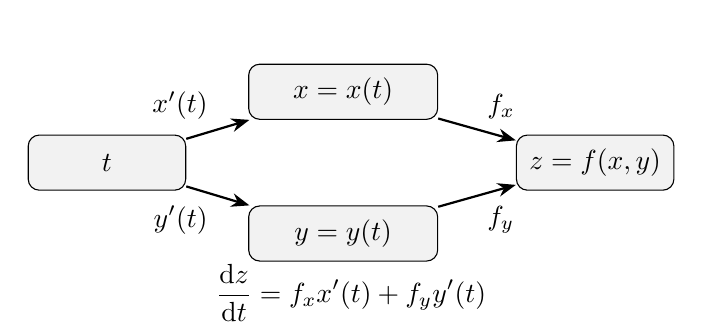
\begin{tikzpicture}[>=Stealth,scale=1.0]
  \node[draw,rounded corners,fill=gray!10,minimum width=2cm,minimum height=0.7cm] (t) at (0,0) {$t$};
  \node[draw,rounded corners,fill=gray!10,minimum width=2.4cm,minimum height=0.7cm] (x) at (3,0.9) {$x=x(t)$};
  \node[draw,rounded corners,fill=gray!10,minimum width=2.4cm,minimum height=0.7cm] (y) at (3,-0.9) {$y=y(t)$};
  \node[draw,rounded corners,fill=gray!10,minimum width=2cm,minimum height=0.7cm] (z) at (6.2,0) {$z=f(x,y)$};
  \draw[->,thick] (t)--(x) node[midway,above left] {$x'(t)$};
  \draw[->,thick] (t)--(y) node[midway,below left] {$y'(t)$};
  \draw[->,thick] (x)--(z) node[midway,above right] {$f_x$};
  \draw[->,thick] (y)--(z) node[midway,below right] {$f_y$};
  \node at (3.1,-1.65) {$\displaystyle \frac{\dd z}{\dd t}=f_xx'(t)+f_yy'(t)$};
\end{tikzpicture}
\end{center}

\begin{example}[多元链式法则]
设
\[
z=x^2y+\sin y,\qquad x=t^2,\qquad y=\ee^t.
\]
求 $\frac{\dd z}{\dd t}$.
\end{example}
\begin{solution}
先求
\[
z_x=2xy,\qquad z_y=x^2+\cos y.
\]
又
\[
\frac{\dd x}{\dd t}=2t,\qquad \frac{\dd y}{\dd t}=\ee^t.
\]
由链式法则，
\[
\frac{\dd z}{\dd t}
=z_x\frac{\dd x}{\dd t}+z_y\frac{\dd y}{\dd t}
=2xy\cdot2t+(x^2+\cos y)\ee^t.
\]
代入 $x=t^2,\ y=\ee^t$，得
\[
\frac{\dd z}{\dd t}
=4t^3\ee^t+(t^4+\cos(\ee^t))\ee^t.
\]
\end{solution}

\begin{theorem}[二元链式法则：二元中间变量情形]
设 $z=f(u,v)$ 在相应点可微，且
\[
u=u(x,y),\qquad v=v(x,y)
\]
在 $(x,y)$ 处有连续偏导数，则复合函数 $z=f(u(x,y),v(x,y))$ 在该点的偏导数为
\[
\frac{\partial z}{\partial x}=f_u\frac{\partial u}{\partial x}+f_v\frac{\partial v}{\partial x},
\qquad
\frac{\partial z}{\partial y}=f_u\frac{\partial u}{\partial y}+f_v\frac{\partial v}{\partial y}.
\]
\end{theorem}
\begin{proofdetail}
只证关于 $x$ 的公式，关于 $y$ 的公式同理. 固定 $y$，令 $x$ 改变为 $x+\Delta x$. 由于 $u,v$ 对 $x$ 可导，
\[
\Delta u=u_x\Delta x+o(\Delta x),\qquad
\Delta v=v_x\Delta x+o(\Delta x).
\]
由 $f$ 在 $(u,v)$ 处可微，
\[
\Delta z=f_u\Delta u+f_v\Delta v+o(\rho),
\qquad \rho=\sqrt{(\Delta u)^2+(\Delta v)^2}.
\]
又 $\Delta u=O(\Delta x),\Delta v=O(\Delta x)$，故 $\rho=O(|\Delta x|)$，从而 $o(\rho)=o(\Delta x)$. 代入得
\[
\Delta z=(f_u u_x+f_v v_x)\Delta x+o(\Delta x).
\]
两边除以 $\Delta x$ 并令 $\Delta x\to0$，得到
\[
\frac{\partial z}{\partial x}=f_u u_x+f_v v_x.
\]
\end{proofdetail}

\begin{example}[二元复合函数偏导]
设 $z=f(x^2+y,xy)$，其中 $f$ 有连续一阶偏导数. 求 $\frac{\partial z}{\partial x}$ 与 $\frac{\partial z}{\partial y}$.
\end{example}
\begin{solution}
令
\[
u=x^2+y,\qquad v=xy.
\]
则 $z=f(u,v)$. 记 $f_u,f_v$ 分别为 $f$ 对第一、第二个变量的偏导数，并在 $(u,v)=(x^2+y,xy)$ 处取值. 由链式法则，
\[
\frac{\partial z}{\partial x}
=f_u\frac{\partial u}{\partial x}+f_v\frac{\partial v}{\partial x}
=2x f_u+y f_v,
\]
\[
\frac{\partial z}{\partial y}
=f_u\frac{\partial u}{\partial y}+f_v\frac{\partial v}{\partial y}
=f_u+x f_v.
\]
\end{solution}


\subsection{偏导数在多参数机器学习模型中的应用}

多元函数的偏导数可以直接解释多参数模型训练. 设有 $m$ 个样本 $(x_i,y_i)$，用一元线性模型
\[
\hat y_i=wx_i+b
\]
进行预测. 常用的均方误差损失为
\[
J(w,b)=\frac{1}{2m}\sum_{i=1}^{m}(wx_i+b-y_i)^2.
\]
这里 $J$ 是关于两个变量 $w,b$ 的函数. 对 $w$ 和 $b$ 分别求偏导，得
\[
\frac{\partial J}{\partial w}
=\frac{1}{m}\sum_{i=1}^{m}(wx_i+b-y_i)x_i,
\qquad
\frac{\partial J}{\partial b}
=\frac{1}{m}\sum_{i=1}^{m}(wx_i+b-y_i).
\]
梯度下降更新为
\[
w_{k+1}=w_k-\eta\frac{\partial J}{\partial w}(w_k,b_k),\qquad
b_{k+1}=b_k-\eta\frac{\partial J}{\partial b}(w_k,b_k).
\]

\begin{example}
对两个样本 $(1,2),(2,3)$，写出线性模型 $\hat y=wx+b$ 的损失函数，并求 $\nabla J(0,0)$.
\end{example}
\begin{solution}
此时 $m=2$，
\[
J(w,b)=\frac14\left[(w+b-2)^2+(2w+b-3)^2\right].
\]
由上面的公式，
\[
\frac{\partial J}{\partial w}
=\frac12\left[(w+b-2)\cdot1+(2w+b-3)\cdot2\right],
\]
\[
\frac{\partial J}{\partial b}
=\frac12\left[(w+b-2)+(2w+b-3)\right].
\]
代入 $(w,b)=(0,0)$，
\[
\frac{\partial J}{\partial w}(0,0)=\frac12[-2+2(-3)]=-4,\qquad
\frac{\partial J}{\partial b}(0,0)=\frac12(-2-3)=-\frac52.
\]
故
\[
\nabla J(0,0)=\left(-4,-\frac52\right).
\]
若学习率为 $\eta$，第一次更新为
\[
(w_1,b_1)=\left(0,0\right)-\eta\left(-4,-\frac52\right)
=\left(4\eta,\frac52\eta\right).
\]
\end{solution}

\subsection{课后习题}
\begin{enumerate}[label=\textbf{练习\arabic*.},leftmargin=2.2em]
\item 判断下列命题真伪，并说明理由：偏导数存在必连续；连续且偏导存在必可微；偏导数连续必可微；可微必连续.
\item 求 $z=x^2y+\ee^{xy}$ 的全微分.
\item 用微分近似计算 $\sqrt{9.06}$.
\item 用微分估计 $\ln(1.02)$.
\item 设 $f(x,y)=x^3y^2+\ee^{xy}$，求 $f_x,f_y,f_{xy},f_{yx}$.
\item 设生产函数 $Q(K,L)=10K^{1/2}L^{1/2}$. 求 $Q_K,Q_L$，并解释它们的意义.
\item 证明函数 $f(x,y)=x^2+y^2-2xy$ 在任意点可微，并写出全微分.
\item 设 $z=x^2y+\sin y,\ x=t^2,\ y=\ee^t$. 求 $\frac{\dd z}{\dd t}$.
\item 设 $z=f(x^2+y,xy)$，其中 $f$ 有连续一阶偏导数. 求 $\frac{\partial z}{\partial x}$ 与 $\frac{\partial z}{\partial y}$.
\item 设
\[
f(x,y)=
\begin{cases}
\dfrac{x^2y}{x^2+y^2},&(x,y)\neq(0,0),\\[0.6em]
0,&(x,y)=(0,0).
\end{cases}
\]
求 $f_x(0,0),f_y(0,0)$，并判断 $f$ 在 $(0,0)$ 是否连续.
\end{enumerate}

\subsection{参考解答}
\begin{enumerate}[label=\textbf{练习\arabic*.},leftmargin=2.2em]
\item 偏导数存在不一定连续，反例可取本章例题
\[
f(x,y)=\frac{xy}{x^2+y^2},\quad f(0,0)=0.
\]
连续且偏导存在不一定可微；例如
\[
f(x,y)=
\begin{cases}
\dfrac{xy}{\sqrt{x^2+y^2}},&(x,y)\neq(0,0),\\[0.6em]
0,&(x,y)=(0,0).
\end{cases}
\]
在原点连续，且
\[
f_x(0,0)=\lim_{h\to0}\frac{f(h,0)-0}{h}=0,\qquad
f_y(0,0)=\lim_{k\to0}\frac{f(0,k)-0}{k}=0.
\]
若它在原点可微，则线性主部应为 $0\cdot x+0\cdot y=0$. 但沿 $y=x$，
\[
\frac{f(x,x)-0}{\sqrt{x^2+x^2}}
=\frac{x^2/\sqrt{2x^2}}{\sqrt{2x^2}}
=\frac12\qquad(x\neq0),
\]
不趋于 $0$，故不可微. 偏导数在邻域内存在且在该点连续可推出可微；可微必连续.
\item
\[
z_x=2xy+y\ee^{xy},\qquad z_y=x^2+x\ee^{xy},
\]
所以
\[
\dd z=(2xy+y\ee^{xy})\dd x+(x^2+x\ee^{xy})\dd y.
\]
\item 取 $f(x)=\sqrt{x}$，在 $x=9$ 处线性化：
\[
\sqrt{9.06}\approx3+\frac{1}{2\sqrt9}\cdot0.06=3.01.
\]
\item 取 $f(x)=\ln x$，在 $x=1$ 处线性化. 因 $f(1)=0,\ f'(1)=1$，且 $\Delta x=0.02$，
\[
\ln(1.02)\approx0+1\cdot0.02=0.02.
\]
\item
\[
f_x=3x^2y^2+y\ee^{xy},\qquad
f_y=2x^3y+x\ee^{xy}.
\]
进一步，
\[
f_{xy}=6x^2y+\ee^{xy}+xy\ee^{xy},
\]
\[
f_{yx}=6x^2y+\ee^{xy}+xy\ee^{xy}.
\]
\item
\[
Q_K=10\cdot\frac12K^{-1/2}L^{1/2}
=5\sqrt{\frac{L}{K}},
\]
\[
Q_L=10\cdot\frac12K^{1/2}L^{-1/2}
=5\sqrt{\frac{K}{L}}.
\]
$Q_K$ 表示劳动投入固定时资本投入增加一单位带来的产出近似增量；$Q_L$ 表示资本投入固定时劳动投入增加一单位带来的产出近似增量.
\item
\[
f_x=2x-2y,\qquad f_y=2y-2x.
\]
二者在全平面连续，故 $f$ 处处可微，且
\[
\dd f=(2x-2y)\dd x+(2y-2x)\dd y.
\]
\item
\[
z_x=2xy,\qquad z_y=x^2+\cos y,
\]
\[
\frac{\dd x}{\dd t}=2t,\qquad \frac{\dd y}{\dd t}=\ee^t.
\]
故
\[
\frac{\dd z}{\dd t}=2xy\cdot2t+(x^2+\cos y)\ee^t.
\]
代入 $x=t^2,\ y=\ee^t$ 得
\[
\frac{\dd z}{\dd t}=4t^3\ee^t+(t^4+\cos(\ee^t))\ee^t.
\]
\item 令 $u=x^2+y,\ v=xy$. 则
\[
\frac{\partial z}{\partial x}=f_u(u,v)\cdot2x+f_v(u,v)\cdot y,
\]
\[
\frac{\partial z}{\partial y}=f_u(u,v)+f_v(u,v)\cdot x,
\]
其中 $(u,v)=(x^2+y,xy)$.
\item 按定义，
\[
f_x(0,0)=\lim_{h\to0}\frac{f(h,0)-f(0,0)}{h}=0,
\]
\[
f_y(0,0)=\lim_{k\to0}\frac{f(0,k)-f(0,0)}{k}=0.
\]
沿任意直线 $y=mx$，
\[
f(x,mx)=\frac{x^2(mx)}{x^2+m^2x^2}
=\frac{mx}{1+m^2}\to0.
\]
但连续性不能只看直线. 由估计
\[
\left|\frac{x^2y}{x^2+y^2}\right|
\leq |y|\frac{x^2}{x^2+y^2}\leq |y|,
\]
当 $(x,y)\to(0,0)$ 时右端趋于 $0$，故 $f$ 在原点连续.
\end{enumerate}

\section{中值定理与洛必达法则}
\renewEnvironmentCounter

本章讨论导数理论中的一组核心桥梁：中值定理. 前几章主要研究“某一点附近”的变化率；中值定理则把区间上的整体变化与某个中间点的导数联系起来. 例如 Lagrange 中值定理说明，只要函数在闭区间上连续、开区间内可导，那么区间两端的平均变化率一定等于某个内点的瞬时变化率.

中值定理的作用主要有三类：
\begin{enumerate}[label=(\arabic*),leftmargin=2em]
\item 证明存在性结论，例如证明某点导数为零、证明方程根的个数；
\item 证明函数不等式，例如比较 $\ln(1+x)$、$\sin x$ 与多项式近似；
\item 推导洛必达法则，用导数之比研究未定式极限.
\end{enumerate}

使用本章定理时，最容易出错的是忽略条件. Rolle 定理要求两端函数值相等；Lagrange 中值定理要求闭区间连续、开区间可导；洛必达法则要求先确认极限是 $0/0$ 型或 $\infty/\infty$ 型，并且导数之比的极限存在.

\subsection{Rolle 定理与 Lagrange 中值定理}

\begin{theorem}[Fermat 引理]
若 $f$ 在 $x_0$ 的某邻域内有定义，在 $x_0$ 处可导，且 $x_0$ 是 $f$ 的局部极值点，则 $f'(x_0)=0$.
\end{theorem}
\begin{proofdetail}
设 $x_0$ 为局部极大点. 存在 $\delta>0$，当 $|h|<\delta$ 时 $f(x_0+h)\leq f(x_0)$. 当 $h>0$ 时，
\[
\frac{f(x_0+h)-f(x_0)}{h}\leq0;
\]
当 $h<0$ 时，由于分母为负，
\[
\frac{f(x_0+h)-f(x_0)}{h}\geq0.
\]
若导数存在，则右极限 $\leq0$，左极限 $\geq0$，二者相等，只能等于 $0$. 局部极小点情形不等号反向，结论同样成立.
\end{proofdetail}

\begin{theorem}[Rolle 定理]
若 $f$ 在 $[a,b]$ 上连续，在 $(a,b)$ 内可导，且 $f(a)=f(b)$，则存在 $\xi\in(a,b)$，使得 $f'(\xi)=0$.
\end{theorem}
\begin{proofdetail}
由闭区间连续函数最值定理，$f$ 在 $[a,b]$ 上取得最大值 $M$ 与最小值 $m$. 若 $M=m$，则 $f$ 为常数，任取 $\xi\in(a,b)$ 有 $f'(\xi)=0$.

若 $M>m$，因 $f(a)=f(b)$，最大值或最小值至少有一个不只在端点取得。具体地，若最大值和最小值都只在端点取得，则端点函数值既等于最大值又等于最小值，矛盾. 因此存在内点 $\xi\in(a,b)$，使 $f$ 在 $\xi$ 处取得局部极大或局部极小. 由 Fermat 引理，$f'(\xi)=0$.
\end{proofdetail}

Rolle 定理的几何意义是：若一段连续光滑曲线的两个端点等高，则曲线内部至少有一点的切线水平.

\begin{center}
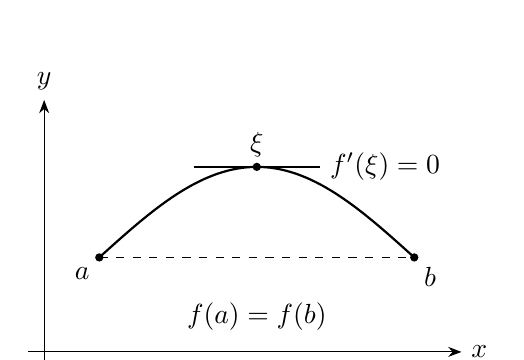
\begin{tikzpicture}[scale=1.0,>=Stealth]
  \draw[->] (-0.2,0)--(5.3,0) node[right] {$x$};
  \draw[->] (0,-0.2)--(0,3.2) node[above] {$y$};
  \draw[domain=0.7:4.7,smooth,variable=\x,thick]
    plot ({\x},{1.2+1.15*sin(45*(\x-0.7))});
  \coordinate (A) at (0.7,1.2);
  \coordinate (B) at (4.7,1.2);
  \coordinate (C) at (2.7,2.35);
  \fill (A) circle (1.5pt) node[below left] {$a$};
  \fill (B) circle (1.5pt) node[below right] {$b$};
  \fill (C) circle (1.5pt) node[above] {$\xi$};
  \draw[dashed] (A)--(B);
  \draw[thick] (1.9,2.35)--(3.5,2.35) node[right] {$f'(\xi)=0$};
  \node at (2.7,0.45) {$f(a)=f(b)$};
\end{tikzpicture}
\end{center}

\begin{theorem}[Lagrange 中值定理]
若 $f$ 在 $[a,b]$ 上连续，在 $(a,b)$ 内可导，则存在 $\xi\in(a,b)$，使得
\[
f'(\xi)=\frac{f(b)-f(a)}{b-a}.
\]
\end{theorem}
\begin{proofdetail}
构造辅助函数
\[
F(x)=f(x)-\frac{f(b)-f(a)}{b-a}(x-a).
\]
$F$ 在 $[a,b]$ 上连续，在 $(a,b)$ 内可导，且
\[
F(a)=f(a),\qquad F(b)=f(b)-[f(b)-f(a)]=f(a).
\]
由 Rolle 定理，存在 $\xi\in(a,b)$ 使 $F'(\xi)=0$. 而
\[
F'(x)=f'(x)-\frac{f(b)-f(a)}{b-a},
\]
故结论成立.
\end{proofdetail}

Lagrange 中值定理的几何意义是：连续光滑曲线上至少有一点的切线平行于连接两端点的弦. 公式
\[
f(b)-f(a)=f'(\xi)(b-a)
\]
说明“总改变量”等于某个中间点的瞬时变化率乘以区间长度.

\begin{center}
\begin{tikzpicture}[scale=1.0,>=Stealth]
  \draw[->] (-0.2,0)--(5.4,0) node[right] {$x$};
  \draw[->] (0,-0.2)--(0,4.0) node[above] {$y$};
  % y=0.18(x-2.2)^2+1, with a=0.8, b=4.6.
  % The secant slope equals f'(2.7)=0.18, so the tangent at xi=2.7 is parallel to the secant.
  \draw[domain=0.55:4.85,smooth,variable=\x,thick]
    plot ({\x},{0.18*(\x-2.2)*(\x-2.2)+1});
  \coordinate (A) at (0.8,1.353);
  \coordinate (B) at (4.6,2.037);
  \coordinate (C) at (2.7,1.045);
  \fill (A) circle (1.5pt) node[below left] {$(a,f(a))$};
  \fill (B) circle (1.5pt) node[above right] {$(b,f(b))$};
  \fill (C) circle (1.5pt) node[below] {$(\xi,f(\xi))$};
  \draw[thick,dashed] (A)--(B) node[midway,above,sloped] {弦};
  \draw[thick] ($(C)+(-1.2,-0.216)$)--($(C)+(1.2,0.216)$) node[right] {切线};
  \draw[dashed] (0.8,0)--(0.8,1.353);
  \draw[dashed] (2.7,0)--(2.7,1.045);
  \draw[dashed] (4.6,0)--(4.6,2.037);
  \node[below] at (0.8,0) {$a$};
  \node[below] at (2.7,0) {$\xi$};
  \node[below] at (4.6,0) {$b$};
\end{tikzpicture}
\end{center}

\begin{example}[验证中值定理]
对 $f(x)=x^2$ 在 $[1,3]$ 上求满足 Lagrange 中值定理的 $\xi$.
\end{example}
\begin{solution}
\[
\frac{f(3)-f(1)}{3-1}=\frac{9-1}{2}=4.
\]
因 $f'(x)=2x$，令 $2\xi=4$ 得 $\xi=2\in(1,3)$.
\end{solution}

\begin{example}[Rolle 定理的条件核查]
判断函数
\[
f(x)=|x|
\]
在区间 $[-1,1]$ 上能否应用 Rolle 定理.
\end{example}
\begin{solution}
首先，
\[
f(-1)=1,\qquad f(1)=1,
\]
两端函数值相等，且 $f$ 在 $[-1,1]$ 上连续. 但是 $f$ 在 $x=0$ 处不可导，因为
\[
\lim_{h\to0+}\frac{|h|-0}{h}=1,\qquad
\lim_{h\to0-}\frac{|h|-0}{h}=-1,
\]
左右导数不相等. 因此 $f$ 不满足“在 $(-1,1)$ 内可导”的条件，不能应用 Rolle 定理.
\end{solution}
\begin{warning}
Rolle 定理的结论不是只由 $f(a)=f(b)$ 推出. 连续性和开区间可导性缺一不可，本题图像有尖点，正好破坏了可导性.
\end{warning}

\begin{example}[Rolle 定理证明方程根的个数]
证明方程
\[
x^3-3x+1=0
\]
在区间 $(-2,2)$ 内有三个不同实根.
\end{example}
\begin{solution}
设
\[
f(x)=x^3-3x+1.
\]
计算得
\[
f(-2)=-1,\quad f(-1)=3,\quad f(0)=1,\quad f(1)=-1,\quad f(2)=3.
\]
由介值定理，区间 $(-2,-1)$、$(0,1)$、$(1,2)$ 内各至少有一个零点，所以 $(-2,2)$ 内至少有三个不同实根.

下面证明不可能有四个或更多不同实根. 若存在四个不同实根
\[
r_1<r_2<r_3<r_4,
\]
则在每个区间 $[r_i,r_{i+1}]$ 上，函数连续、开区间内可导，且两端函数值都为 $0$. 由 Rolle 定理，$f'$ 在 $(r_1,r_2)$、$(r_2,r_3)$、$(r_3,r_4)$ 内各至少有一个零点，因此 $f'$ 至少有三个不同零点. 但
\[
f'(x)=3x^2-3=3(x-1)(x+1)
\]
只有两个零点 $-1,1$，矛盾. 故方程在 $(-2,2)$ 内恰有三个不同实根.
\end{solution}

\begin{example}[构造辅助函数]
设 $f$ 在 $[0,1]$ 上连续，在 $(0,1)$ 内可导，且 $f(1)=0$. 证明存在 $\xi\in(0,1)$，使得
\[
f'(\xi)=-\frac{f(\xi)}{\xi}.
\]
\end{example}
\begin{solution}
令
\[
F(x)=xf(x).
\]
则 $F$ 在 $[0,1]$ 上连续，在 $(0,1)$ 内可导，并且
\[
F(0)=0,\qquad F(1)=f(1)=0.
\]
由 Rolle 定理，存在 $\xi\in(0,1)$，使得 $F'(\xi)=0$. 而
\[
F'(x)=f(x)+xf'(x),
\]
所以
\[
f(\xi)+\xi f'(\xi)=0.
\]
由于 $\xi\in(0,1)$，可除以 $\xi$，得到
\[
f'(\xi)=-\frac{f(\xi)}{\xi}.
\]
\end{solution}

\begin{example}[构造辅助函数]
设 $f$ 在 $[a,b]$ 上连续，在 $(a,b)$ 内可导，且 $f(a)=f(b)=0$. 证明存在 $\xi\in(a,b)$，使得
\[
f'(\xi)+f(\xi)=0.
\]
\end{example}
\begin{solution}
观察到表达式 $f'(x)+f(x)$ 是 $\ee^x f(x)$ 的导数中除去正因子后的部分. 令
\[
F(x)=\ee^x f(x).
\]
则 $F$ 在 $[a,b]$ 上连续，在 $(a,b)$ 内可导，并且
\[
F(a)=\ee^a f(a)=0,\qquad F(b)=\ee^b f(b)=0.
\]
由 Rolle 定理，存在 $\xi\in(a,b)$，使得 $F'(\xi)=0$. 而
\[
F'(x)=\ee^x f(x)+\ee^x f'(x)=\ee^x[f'(x)+f(x)].
\]
由于 $\ee^\xi>0$，所以
\[
f'(\xi)+f(\xi)=0.
\]
\end{solution}

\begin{example}[由导数界估计函数增量]
设 $f$ 在 $[a,b]$ 上连续，在 $(a,b)$ 内可导，且存在常数 $M>0$，使得
\[
|f'(x)|\leq M,\qquad x\in(a,b).
\]
证明对任意 $x_1,x_2\in[a,b]$，有
\[
|f(x_2)-f(x_1)|\leq M|x_2-x_1|.
\]
\end{example}
\begin{solution}
若 $x_1=x_2$，结论成立. 设 $x_1<x_2$. 由 Lagrange 中值定理，存在 $\xi\in(x_1,x_2)$，使得
\[
f(x_2)-f(x_1)=f'(\xi)(x_2-x_1).
\]
取绝对值得
\[
|f(x_2)-f(x_1)|=|f'(\xi)|\,|x_2-x_1|\leq M|x_2-x_1|.
\]
当 $x_1>x_2$ 时交换两点即可.
\end{solution}

\subsection{Cauchy 中值定理与若干推论}

\begin{theorem}[Cauchy 中值定理]
若 $f,g$ 在 $[a,b]$ 上连续，在 $(a,b)$ 内可导，且 $g'(x)\neq0$ 对所有 $x\in(a,b)$ 成立，则存在 $\xi\in(a,b)$，使得
\[
\frac{f'(\xi)}{g'(\xi)}=\frac{f(b)-f(a)}{g(b)-g(a)}.
\]
\end{theorem}
\begin{proofdetail}
先说明 $g(b)\neq g(a)$. 若 $g(b)=g(a)$，由 Rolle 定理存在 $\eta\in(a,b)$ 使 $g'(\eta)=0$，与条件矛盾.

构造
\[
F(x)=f(x)-f(a)-\frac{f(b)-f(a)}{g(b)-g(a)}[g(x)-g(a)].
\]
则 $F$ 在 $[a,b]$ 连续，在 $(a,b)$ 可导，且 $F(a)=F(b)=0$. 由 Rolle 定理，存在 $\xi\in(a,b)$ 使 $F'(\xi)=0$. 即
\[
f'(\xi)-\frac{f(b)-f(a)}{g(b)-g(a)}g'(\xi)=0.
\]
因 $g'(\xi)\neq0$，除以 $g'(\xi)$ 得结论.
\end{proofdetail}

\begin{proposition}[导数恒为零的函数为常数]
若 $f$ 在区间 $I$ 上可导，且 $f'(x)=0$ 对所有 $x\in I$ 成立，则 $f$ 在 $I$ 上为常数.
\end{proposition}
\begin{proofdetail}
任取 $x_1,x_2\in I$，不妨 $x_1<x_2$. $f$ 在 $[x_1,x_2]$ 连续、在 $(x_1,x_2)$ 可导. 由 Lagrange 中值定理，存在 $\xi\in(x_1,x_2)$ 使
\[
f(x_2)-f(x_1)=f'(\xi)(x_2-x_1)=0.
\]
故任意两点函数值相等，$f$ 为常数.
\end{proofdetail}

\begin{proposition}[导数相等的函数相差常数]
若 $f,g$ 在区间 $I$ 上可导，且
\[
f'(x)=g'(x),\qquad x\in I,
\]
则存在常数 $C$，使得
\[
f(x)=g(x)+C,\qquad x\in I.
\]
\end{proposition}
\begin{proofdetail}
令 $h(x)=f(x)-g(x)$. 则 $h$ 在 $I$ 上可导，且
\[
h'(x)=f'(x)-g'(x)=0.
\]
由“导数恒为零的函数为常数”，$h(x)=C$. 即
\[
f(x)-g(x)=C.
\]
\end{proofdetail}

\begin{example}[Cauchy 中值定理验证]
设
\[
f(x)=\ln x,\qquad g(x)=x,\qquad x\in[1,\ee].
\]
求 Cauchy 中值定理中的 $\xi$.
\end{example}
\begin{solution}
$f,g$ 在 $[1,\ee]$ 上连续，在 $(1,\ee)$ 内可导，且 $g'(x)=1\neq0$. Cauchy 中值定理给出存在 $\xi\in(1,\ee)$，使
\[
\frac{f'(\xi)}{g'(\xi)}
=\frac{f(\ee)-f(1)}{g(\ee)-g(1)}.
\]
即
\[
\frac{1/\xi}{1}=\frac{1-0}{\ee-1}=\frac1{\ee-1}.
\]
因此
\[
\xi=\ee-1.
\]
由于 $1<\ee-1<\ee$，该点确在区间内部.
\end{solution}

\begin{example}[用 Cauchy 中值定理证明不等式]
证明当 $0<a<b$ 时，
\[
\frac{b-a}{b}<\ln b-\ln a<\frac{b-a}{a}.
\]
\end{example}
\begin{solution}
对 $f(x)=\ln x$ 和 $g(x)=x$ 在 $[a,b]$ 上应用 Cauchy 中值定理，存在 $\xi\in(a,b)$，使得
\[
\frac{\ln b-\ln a}{b-a}=\frac{f'(\xi)}{g'(\xi)}=\frac1{\xi}.
\]
因为 $a<\xi<b$，所以
\[
\frac1b<\frac1\xi<\frac1a.
\]
又 $b-a>0$，两边同乘以 $b-a$ 得
\[
\frac{b-a}{b}<\ln b-\ln a<\frac{b-a}{a}.
\]
\end{solution}

\begin{example}[不等式]
证明当 $x>0$ 时，$\ln(1+x)<x$.
\end{example}
\begin{solution}
令 $f(t)=\ln(1+t)$，在 $[0,x]$ 上应用 Lagrange 中值定理，存在 $\xi\in(0,x)$ 使
\[
\ln(1+x)-\ln1=f'(\xi)x=\frac{x}{1+\xi}.
\]
因 $\xi>0$，有 $1+\xi>1$，故 $\ln(1+x)=x/(1+\xi)<x$.
\end{solution}

\begin{example}[不等式]
证明当 $x>0$ 时，
\[
\ln(1+x)>\frac{x}{1+x}.
\]
\end{example}
\begin{solution}
令
\[
F(x)=\ln(1+x)-\frac{x}{1+x},\qquad x\geq0.
\]
有 $F(0)=0$，且当 $x>0$ 时
\[
F'(x)=\frac1{1+x}-\frac1{(1+x)^2}
=\frac{x}{(1+x)^2}>0.
\]
由单调性判别法，$F$ 在 $[0,\infty)$ 上单调增加. 因此对 $x>0$，
\[
F(x)>F(0)=0,
\]
即
\[
\ln(1+x)>\frac{x}{1+x}.
\]
\end{solution}

\begin{example}[三角函数不等式]
证明当 $x>0$ 时，
\[
\sin x<x.
\]
\end{example}
\begin{solution}
当 $x\geq\pi$ 时，$\sin x\leq1<x$，结论成立. 下面只需考虑 $0<x<\pi$.

令 $f(t)=\sin t$，在 $[0,x]$ 上应用 Lagrange 中值定理，存在 $\xi\in(0,x)$，使得
\[
\sin x-\sin0=f'(\xi)x=\cos\xi\,x.
\]
由于 $0<\xi<\pi$，有 $\cos\xi<1$，故
\[
\sin x=x\cos\xi<x.
\]
\end{solution}

\begin{example}[指数函数不等式]
证明对一切实数 $x$，
\[
\ee^x\geq1+x,
\]
且等号当且仅当 $x=0$.
\end{example}
\begin{solution}
令
\[
F(x)=\ee^x-1-x.
\]
则
\[
F'(x)=\ee^x-1.
\]
当 $x<0$ 时，$F'(x)<0$；当 $x>0$ 时，$F'(x)>0$. 因而 $F$ 在 $(-\infty,0)$ 上单调减少，在 $(0,\infty)$ 上单调增加，所以 $x=0$ 是全局最小点. 又
\[
F(0)=0.
\]
于是 $F(x)\geq0$，即
\[
\ee^x\geq1+x.
\]
当 $x\neq0$ 时，$F(x)>F(0)=0$，故等号仅当 $x=0$ 成立.
\end{solution}

\subsection{洛必达法则}

\begin{theorem}[洛必达法则：$0/0$ 型]
设 $f,g$ 在 $a$ 的某去心右邻域内可导，且 $g'(x)\neq0$. 若
\[
\lim_{x\to a+}f(x)=\lim_{x\to a+}g(x)=0,\qquad
\lim_{x\to a+}\frac{f'(x)}{g'(x)}=L
\]
其中 $L$ 可为有限数或无穷大，则
\[
\lim_{x\to a+}\frac{f(x)}{g(x)}=L.
\]
左极限、双侧极限与 $x\to\infty$ 的相应形式类似成立.
\end{theorem}
\begin{proofdetail}
先证 $L$ 为有限数的情形. 任取 $\varepsilon>0$，由 $\frac{f'}{g'}\to L$，存在 $\delta>0$，当 $a<x<a+\delta$ 时，
\[
L-\varepsilon<\frac{f'(x)}{g'(x)}<L+\varepsilon.
\]
取 $x\in(a,a+\delta)$，再取 $t\in(a,x)$. 在 $[t,x]$ 上对 $f,g$ 应用 Cauchy 中值定理，存在 $\xi\in(t,x)$ 使
\[
\frac{f(x)-f(t)}{g(x)-g(t)}=\frac{f'(\xi)}{g'(\xi)}.
\]
因此
\[
\left|\frac{f(x)-f(t)}{g(x)-g(t)}-L\right|<\varepsilon.
\]
固定 $x$ 后令 $t\to a+$，由 $f(t)\to0,g(t)\to0$ 得
\[
\left|\frac{f(x)}{g(x)}-L\right|\leq\varepsilon
\]
其中 $x\in(a,a+\delta)$ 且 $g(x)\neq0$. 因 $\varepsilon$ 任意，得 $\frac{f(x)}{g(x)}\to L$.

若 $L=+\infty$，对任意 $M>0$，存在 $\delta>0$ 使 $a<x<a+\delta$ 时 $\frac{f'(x)}{g'(x)}>M$. 重复上面的 Cauchy 中值定理步骤，令 $t\to a+$ 得 $\frac{f(x)}{g(x)}>M$，故极限为 $+\infty$. $L=-\infty$ 同理.
\end{proofdetail}

\begin{theorem}[洛必达法则：$\infty/\infty$ 型]
设 $f,g$ 在 $a$ 的某去心右邻域内可导，且 $g'(x)\neq0$. 若
\[
\lim_{x\to a+}|f(x)|=+\infty,\qquad
\lim_{x\to a+}|g(x)|=+\infty,
\]
并且
\[
\lim_{x\to a+}\frac{f'(x)}{g'(x)}=L,
\]
其中 $L$ 可为有限数或无穷大，则
\[
\lim_{x\to a+}\frac{f(x)}{g(x)}=L.
\]
左极限、双侧极限与 $x\to\infty$ 的相应形式类似成立.
\end{theorem}
\begin{proofdetail}
证明有限 $L$ 的情形. 任取 $\varepsilon>0$，由 $\frac{f'}{g'}\to L$，存在去心右邻域，使得其中任意点 $u$ 都满足
\[
\left|\frac{f'(u)}{g'(u)}-L\right|<\varepsilon.
\]
固定该邻域内一点 $x_0$. 对 $x$ 与 $x_0$ 之间的闭区间应用 Cauchy 中值定理，存在 $\xi$ 介于 $x$ 与 $x_0$ 之间，使
\[
\frac{f(x)-f(x_0)}{g(x)-g(x_0)}=\frac{f'(\xi)}{g'(\xi)}.
\]
当 $x\to a+$ 时，$\xi\to a+$，所以
\[
\frac{f(x)-f(x_0)}{g(x)-g(x_0)}\to L.
\]
又因为 $|f(x)|,|g(x)|\to\infty$，有
\[
\frac{f(x)}{g(x)}
=\frac{f(x)-f(x_0)}{g(x)-g(x_0)}
\cdot
\frac{1-\frac{f(x_0)}{f(x)}}{1-\frac{g(x_0)}{g(x)}}.
\]
第二个因子趋于 $1$，故 $\frac{f(x)}{g(x)}\to L$. $L$ 为无穷大的情形可仿照 $0/0$ 型证明，用任意大数估计完成.
\end{proofdetail}

\begin{example}[$0/0$ 型]
求 $\displaystyle\lim_{x\to0}\frac{\sin x}{x}$.
\end{example}
\begin{solution}
这是 $0/0$ 型. 用洛必达法则：
\[
\lim_{x\to0}\frac{\sin x}{x}=\lim_{x\to0}\frac{\cos x}{1}=1.
\]
\end{solution}

\begin{example}[多次使用]
求 $\displaystyle\lim_{x\to0}\frac{\ee^x-1-x}{x^2}$.
\end{example}
\begin{solution}
第一次洛必达：
\[
\lim_{x\to0}\frac{\ee^x-1-x}{x^2}
=\lim_{x\to0}\frac{\ee^x-1}{2x}.
\]
仍为 $0/0$ 型，第二次洛必达：
\[
=\lim_{x\to0}\frac{\ee^x}{2}=\frac12.
\]
\end{solution}
\begin{warning}
使用洛必达前必须确认是 $0/0$ 或 $\infty/\infty$ 型，并确认分母导数不为零的条件在去心邻域内成立.
\end{warning}

\begin{example}[$\infty/\infty$ 型]
求
\[
\lim_{x\to\infty}\frac{\ln x}{x^\alpha},\qquad \alpha>0.
\]
\end{example}
\begin{solution}
当 $x\to\infty$ 时，分子、分母都趋于 $+\infty$，属于 $\infty/\infty$ 型. 用洛必达法则：
\[
\lim_{x\to\infty}\frac{\ln x}{x^\alpha}
=\lim_{x\to\infty}\frac{1/x}{\alpha x^{\alpha-1}}
=\lim_{x\to\infty}\frac{1}{\alpha x^\alpha}=0.
\]
这说明任意正幂函数 $x^\alpha$ 的增长都快于 $\ln x$.
\end{solution}

\begin{example}[三角函数高阶小量]
求
\[
\lim_{x\to0}\frac{\tan x-x}{x^3}.
\]
\end{example}
\begin{solution}
这是 $0/0$ 型. 第一次洛必达：
\[
\lim_{x\to0}\frac{\tan x-x}{x^3}
=\lim_{x\to0}\frac{\sec^2x-1}{3x^2}
=\lim_{x\to0}\frac{\tan^2x}{3x^2}.
\]
因为 $\lim_{x\to0}\frac{\tan x}{x}=1$，所以
\[
\lim_{x\to0}\frac{\tan^2x}{3x^2}
=\frac13.
\]
\end{solution}

\begin{example}[不能机械使用洛必达法则]
讨论 $\displaystyle\lim_{x\to\infty}\frac{x+\sin x}{x+\cos x}$.
\end{example}
\begin{solution}
这是 $\infty/\infty$ 型，但直接看导数之比会得到
\[
\frac{(x+\sin x)'}{(x+\cos x)'}=\frac{1+\cos x}{1-\sin x},
\]
该式当 $x\to\infty$ 时无极限，因此不能由洛必达法则推出原极限不存在. 原式应先整理：
\[
\frac{x+\sin x}{x+\cos x}
=\frac{1+\frac{\sin x}{x}}{1+\frac{\cos x}{x}}.
\]
由于 $\sin x/x\to0,\ \cos x/x\to0$，原极限为 $1$.
\end{solution}
\begin{warning}
洛必达法则给出的是充分条件：若导数之比的极限存在，原比值极限等于它. 导数之比极限不存在时，原极限仍可能存在.
\end{warning}

\begin{example}[转化未定式]
求 $\displaystyle\lim_{x\to0+}x\ln x$.
\end{example}
\begin{solution}
原式为 $0\cdot(-\infty)$ 型，改写为
\[
x\ln x=\frac{\ln x}{1/x}.
\]
当 $x\to0+$ 时为 $-\infty/\infty$ 型. 用洛必达法则：
\[
\lim_{x\to0+}\frac{\ln x}{1/x}
=\lim_{x\to0+}\frac{1/x}{-1/x^2}
=\lim_{x\to0+}(-x)=0.
\]
\end{solution}

\begin{example}[指数型未定式]
求
\[
\lim_{x\to0+}x^x.
\]
\end{example}
\begin{solution}
原式为 $0^0$ 型. 设
\[
y=x^x.
\]
取对数得
\[
\ln y=x\ln x.
\]
由上一例，
\[
\lim_{x\to0+}x\ln x=0.
\]
因此
\[
\lim_{x\to0+}\ln y=0.
\]
由于指数函数连续，
\[
\lim_{x\to0+}x^x=\ee^0=1.
\]
\end{solution}

\begin{example}[差型未定式]
求
\[
\lim_{x\to0+}\left(\frac1x-\frac1{\ee^x-1}\right).
\]
\end{example}
\begin{solution}
原式为 $\infty-\infty$ 型，先通分：
\[
\frac1x-\frac1{\ee^x-1}
=\frac{\ee^x-1-x}{x(\ee^x-1)}.
\]
当 $x\to0+$ 时为 $0/0$ 型. 用洛必达法则：
\[
\lim_{x\to0+}\frac{\ee^x-1-x}{x(\ee^x-1)}
=\lim_{x\to0+}\frac{\ee^x-1}{\ee^x-1+x\ee^x}.
\]
仍为 $0/0$ 型，再用一次洛必达：
\[
=\lim_{x\to0+}\frac{\ee^x}{2\ee^x+x\ee^x}
=\frac12.
\]
\end{solution}

\begin{example}[参数型极限]
设 $a>0$. 求
\[
\lim_{x\to0}\frac{a^x-1}{x}.
\]
\end{example}
\begin{solution}
当 $x\to0$ 时为 $0/0$ 型. 由洛必达法则，
\[
\lim_{x\to0}\frac{a^x-1}{x}
=\lim_{x\to0}\frac{a^x\ln a}{1}
=\ln a.
\]
特别地，当 $a=\ee$ 时，得到
\[
\lim_{x\to0}\frac{\ee^x-1}{x}=1.
\]
\end{solution}

\subsection{课后习题}
\begin{enumerate}[label=\textbf{练习\arabic*.},leftmargin=2.2em]
\item 判断下列函数在给定区间上能否应用 Rolle 定理；若能，求出满足结论的点：
\[
f(x)=x^2-1,\ [-1,1];\qquad
g(x)=|x|,\ [-1,1].
\]
\item 对函数 $f(x)=x^3$ 在区间 $[-1,2]$ 上求满足 Lagrange 中值定理的 $\xi$.
\item 设 $f$ 在 $[0,1]$ 上连续，在 $(0,1)$ 内可导，且 $f(0)=f(1)$. 证明存在 $\xi\in(0,1)$，使得
\[
f'(\xi)=0.
\]
\item 设 $f$ 在 $[a,b]$ 上连续，在 $(a,b)$ 内可导，且 $f(a)=f(b)=0$. 证明存在 $\xi\in(a,b)$，使得
\[
f'(\xi)+f(\xi)=0.
\]
\item 证明当 $x>0$ 时，
\[
\frac{x}{1+x}<\ln(1+x)<x.
\]
\item 证明对一切实数 $x$，有
\[
\ee^x\geq1+x.
\]
\item 证明当 $0<a<b$ 时，
\[
\frac{b-a}{b}<\ln b-\ln a<\frac{b-a}{a}.
\]
\item 求极限：
\[
\lim_{x\to0}\frac{\tan x-x}{x^3},\qquad
\lim_{x\to0}\frac{\ee^x-1-x}{x^2}.
\]
\item 求极限：
\[
\lim_{x\to\infty}\frac{\ln x}{\sqrt{x}},\qquad
\lim_{x\to0+}x\ln x.
\]
\item 求极限：
\[
\lim_{x\to0+}x^x,\qquad
\lim_{x\to0+}\left(\frac1x-\frac1{\ee^x-1}\right).
\]
\item 设 $a>0$，求
\[
\lim_{x\to0}\frac{a^x-1}{x}.
\]
\item 讨论
\[
\lim_{x\to\infty}\frac{x+\sin x}{x+\cos x},
\]
并说明为什么不能因导数之比无极限就断定原极限不存在.
\end{enumerate}

\subsection{参考解答}
\begin{enumerate}[label=\textbf{练习\arabic*.},leftmargin=2.2em]
\item $f(x)=x^2-1$ 在 $[-1,1]$ 上连续、在 $(-1,1)$ 内可导，且 $f(-1)=f(1)=0$，可用 Rolle 定理. 由
\[
f'(x)=2x
\]
得 $\xi=0$. 函数 $g(x)=|x|$ 虽在 $[-1,1]$ 上连续且 $g(-1)=g(1)$，但在 $0$ 处不可导，不能应用 Rolle 定理.
\item
\[
\frac{f(2)-f(-1)}{2-(-1)}=\frac{8-(-1)}{3}=3.
\]
而 $f'(x)=3x^2$，令 $3\xi^2=3$，得 $\xi=\pm1$. 由于 $\xi\in(-1,2)$，故只有 $\xi=1$ 满足.
\item 这正是 Rolle 定理. 由于 $f$ 在 $[0,1]$ 上连续、在 $(0,1)$ 内可导，且 $f(0)=f(1)$，存在 $\xi\in(0,1)$ 使 $f'(\xi)=0$.
\item 令 $F(x)=\ee^x f(x)$. 则 $F(a)=F(b)=0$，由 Rolle 定理存在 $\xi$ 使
\[
F'(\xi)=\ee^\xi[f'(\xi)+f(\xi)]=0.
\]
由于 $\ee^\xi>0$，故 $f'(\xi)+f(\xi)=0$.
\item 左侧可令
\[
F(x)=\ln(1+x)-\frac{x}{1+x}.
\]
则 $F(0)=0$，且
\[
F'(x)=\frac{x}{(1+x)^2}>0\qquad(x>0),
\]
所以 $F(x)>0$. 右侧由 Lagrange 中值定理得
\[
\ln(1+x)=\frac{x}{1+\xi}<x,\qquad 0<\xi<x.
\]
\item 令 $F(x)=\ee^x-1-x$. 则 $F'(x)=\ee^x-1$. $F$ 在 $(-\infty,0)$ 上递减，在 $(0,\infty)$ 上递增，故 $F(0)=0$ 为全局最小值. 因此 $\ee^x\geq1+x$.
\item 对 $f(x)=\ln x$、$g(x)=x$ 在 $[a,b]$ 上应用 Cauchy 中值定理，存在 $\xi\in(a,b)$，使
\[
\frac{\ln b-\ln a}{b-a}=\frac1\xi.
\]
由 $a<\xi<b$，得
\[
\frac1b<\frac1\xi<\frac1a.
\]
同乘 $b-a>0$ 即得结论.
\item
\[
\lim_{x\to0}\frac{\tan x-x}{x^3}
=\lim_{x\to0}\frac{\sec^2x-1}{3x^2}
=\lim_{x\to0}\frac{\tan^2x}{3x^2}=\frac13.
\]
又
\[
\lim_{x\to0}\frac{\ee^x-1-x}{x^2}
=\lim_{x\to0}\frac{\ee^x-1}{2x}
=\lim_{x\to0}\frac{\ee^x}{2}=\frac12.
\]
\item
\[
\lim_{x\to\infty}\frac{\ln x}{\sqrt{x}}
=\lim_{x\to\infty}\frac{1/x}{1/(2\sqrt{x})}
=\lim_{x\to\infty}\frac{2}{\sqrt{x}}=0.
\]
另外
\[
\lim_{x\to0+}x\ln x
=\lim_{x\to0+}\frac{\ln x}{1/x}
=\lim_{x\to0+}\frac{1/x}{-1/x^2}
=\lim_{x\to0+}(-x)=0.
\]
\item
\[
x^x=\ee^{x\ln x},\qquad x\ln x\to0,
\]
所以 $\lim_{x\to0+}x^x=1$. 其次
\[
\frac1x-\frac1{\ee^x-1}
=\frac{\ee^x-1-x}{x(\ee^x-1)}.
\]
两次洛必达得
\[
\lim_{x\to0+}\frac{\ee^x-1-x}{x(\ee^x-1)}
=\lim_{x\to0+}\frac{\ee^x-1}{\ee^x-1+x\ee^x}
=\lim_{x\to0+}\frac{\ee^x}{2\ee^x+x\ee^x}
=\frac12.
\]
\item
\[
\lim_{x\to0}\frac{a^x-1}{x}
=\lim_{x\to0}a^x\ln a=\ln a.
\]
\item
\[
\frac{x+\sin x}{x+\cos x}
=\frac{1+\frac{\sin x}{x}}{1+\frac{\cos x}{x}}\to1.
\]
导数之比为
\[
\frac{1+\cos x}{1-\sin x},
\]
它没有极限. 洛必达法则只能说“若导数之比极限存在，则原极限等于它”，不能反过来由导数之比无极限推出原极限不存在.
\end{enumerate}

\section{导数的应用}
\renewEnvironmentCounter
\subsection{函数单调性判别法}

\begin{theorem}[单调性判别法]
设 $f$ 在区间 $I$ 上连续，在 $I$ 的内部可导. 若 $f'(x)\geq0$ 对内部所有点成立，则 $f$ 在 $I$ 上单调不减；若 $f'(x)>0$ 对内部所有点成立，则 $f$ 在 $I$ 上严格单调增加. 相应地，$f'(x)\leq0$ 推出单调不增，$f'(x)<0$ 推出严格单调减少.
\end{theorem}
\begin{proofdetail}
任取 $x_1<x_2$，由 Lagrange 中值定理，存在 $\xi\in(x_1,x_2)$，使
\[
f(x_2)-f(x_1)=f'(\xi)(x_2-x_1).
\]
若 $f'\geq0$，则右端 $\geq0$，故 $f(x_2)\geq f(x_1)$. 若 $f'>0$，则右端 $>0$，故严格增加. 其余情形同理.
\end{proofdetail}

\begin{example}[求单调区间]
求 $f(x)=x^3-3x$ 的单调区间.
\end{example}
\begin{solution}
\[
f'(x)=3x^2-3=3(x-1)(x+1).
\]
当 $x<-1$ 或 $x>1$ 时 $f'(x)>0$；当 $-1<x<1$ 时 $f'(x)<0$. 故 $f$ 在 $(-\infty,-1)$ 与 $(1,\infty)$ 上单调增加，在 $(-1,1)$ 上单调减少.
\end{solution}

\begin{example}[求单调区间]
求函数
\[
f(x)=2x^3-9x^2+12x-3
\]
的单调区间.
\end{example}
\begin{solution}
\[
f'(x)=6x^2-18x+12=6(x-1)(x-2).
\]
临界点为 $x=1,2$. 当 $x<1$ 时 $f'(x)>0$；当 $1<x<2$ 时 $f'(x)<0$；当 $x>2$ 时 $f'(x)>0$. 因此 $f$ 在 $(-\infty,1)$ 与 $(2,\infty)$ 上单调增加，在 $(1,2)$ 上单调减少.
\end{solution}

\subsection{函数的极值}

\begin{definition}[局部极值]
若存在 $\delta>0$，使得对所有满足 $|x-x_0|<\delta$ 的 $x$，都有 $f(x)\leq f(x_0)$，则称 $f(x_0)$ 为局部极大值. 若不等号反向，则称为局部极小值.
\end{definition}

\begin{theorem}[一阶导数变号判别法]
设 $f$ 在 $x_0$ 连续，在 $x_0$ 的去心邻域内可导. 若 $f'$ 在 $x_0$ 左侧为正、右侧为负，则 $f(x_0)$ 为局部极大值；若左侧为负、右侧为正，则为局部极小值；若左右不变号，则不是极值点.
\end{theorem}
\begin{proofdetail}
只证由正变负的情形. 存在 $\delta>0$，使 $f'(x)>0$ 对 $x\in(x_0-\delta,x_0)$ 成立，$f'(x)<0$ 对 $x\in(x_0,x_0+\delta)$ 成立. 由单调性判别法，$f$ 在左侧区间单调增加，在右侧区间单调减少. 因 $f$ 在 $x_0$ 连续，对任意 $x\in(x_0-\delta,x_0)$ 有 $f(x)<f(x_0)$，对任意 $x\in(x_0,x_0+\delta)$ 有 $f(x)<f(x_0)$. 因此 $f(x_0)$ 为局部极大值. 其余情形同理.
\end{proofdetail}

\begin{theorem}[二阶导数判别法]
设 $f'(x_0)=0$，且 $f''(x_0)$ 存在. 若 $f''(x_0)>0$，则 $f(x_0)$ 是局部极小值；若 $f''(x_0)<0$，则是局部极大值.
\end{theorem}
\begin{proofdetail}
由二阶导数定义，
\[
f''(x_0)=\lim_{x\to x_0}\frac{f'(x)-f'(x_0)}{x-x_0}
=\lim_{x\to x_0}\frac{f'(x)}{x-x_0}.
\]
若 $f''(x_0)>0$，则存在 $\delta>0$，当 $0<|x-x_0|<\delta$ 时
\[
\frac{f'(x)}{x-x_0}>0.
\]
于是 $x<x_0$ 时 $f'(x)<0$，$x>x_0$ 时 $f'(x)>0$，由一阶变号判别法得局部极小. $f''(x_0)<0$ 时同理得到导数由正变负，故为局部极大.
\end{proofdetail}

\begin{example}[极值]
求 $f(x)=x^4-4x^3$ 的极值.
\end{example}
\begin{solution}
\[
f'(x)=4x^3-12x^2=4x^2(x-3).
\]
临界点为 $x=0,3$. 因 $x^2\geq0$，$f'(x)$ 在 $0$ 两侧均为负，所以 $x=0$ 不是极值点. $f'$ 在 $3$ 左侧负、右侧正，故 $x=3$ 为局部极小点，
\[
f(3)=81-108=-27.
\]
\end{solution}
\begin{warning}
导数为零只是极值的必要条件，不是充分条件. $x=0$ 就是典型反例.
\end{warning}

\begin{example}[极值]
求函数
\[
f(x)=(x-1)^2(x+1)^3
\]
的极值.
\end{example}
\begin{solution}
求导得
\[
f'(x)=2(x-1)(x+1)^3+3(x-1)^2(x+1)^2
=(x-1)(x+1)^2(5x-1).
\]
临界点为 $x=-1,\frac15,1$. 由于 $(x+1)^2\geq0$，且除 $x=-1$ 外不改变符号，只需考察 $(x-1)(5x-1)$ 的符号，并注意 $x=-1$ 两侧符号是否改变.

当 $x<\frac15$ 且 $x\neq-1$ 时，$(x-1)<0,\ 5x-1<0$，故 $f'(x)>0$；当 $\frac15<x<1$ 时，$f'(x)<0$；当 $x>1$ 时，$f'(x)>0$. 因而 $x=-1$ 不是极值点，$x=\frac15$ 为局部极大点，$x=1$ 为局部极小点.

函数值为
\[
f\left(\frac15\right)=\left(-\frac45\right)^2\left(\frac65\right)^3=\frac{3456}{3125},\qquad
f(1)=0.
\]
故局部极大值为 $\frac{3456}{3125}$，局部极小值为 $0$.
\end{solution}

\subsection{函数的最值与应用优化}

\begin{proposition}[闭区间最值求法]
若 $f$ 在 $[a,b]$ 连续，则最大值和最小值只能在端点、不可导点或内部驻点 $f'(x)=0$ 处取得. 逐一比较这些点的函数值即可.
\end{proposition}
\begin{proofdetail}
最值存在性来自闭区间连续函数最值定理. 若最值在内部点 $x_0$ 取得且 $f$ 在 $x_0$ 可导，则由 Fermat 引理 $f'(x_0)=0$. 若内部点不可导，也必须列入候选. 端点处 Fermat 引理不适用，因此端点也必须比较.
\end{proofdetail}

\begin{example}[利润最大化]
某产品价格与销量满足 $p(q)=100-q$，成本 $C(q)=20q+100$，其中 $0\leq q\leq100$. 求最大利润.
\end{example}
\begin{solution}
收入 $R(q)=qp(q)=100q-q^2$，利润
\[
\Pi(q)=R(q)-C(q)=80q-q^2-100.
\]
\[
\Pi'(q)=80-2q.
\]
令 $\Pi'(q)=0$ 得 $q=40$. 比较
\[
\Pi(0)=-100,\quad \Pi(40)=1600-100=1500,\quad \Pi(100)=8000-10000-100=-2100.
\]
最大利润为 $1500$，在 $q=40$ 时取得.
\end{solution}

\begin{example}[证明方程根的个数]
证明方程 $x^3-3x+1=0$ 在区间 $(-2,2)$ 内有三个不同实根.
\end{example}
\begin{solution}
设 $f(x)=x^3-3x+1$. 有
\[
f(-2)=-1,\quad f(-1)=3,\quad f(0)=1,\quad f(1)=-1,\quad f(2)=3.
\]
由介值定理，$(-2,-1)$、$(0,1)$、$(1,2)$ 内各至少有一个根.

再证至多三个根. 若有四个不同实根 $r_1<r_2<r_3<r_4$，由 Rolle 定理，$f'$ 在三个相邻根之间至少有三个不同零点. 但
\[
f'(x)=3x^2-3
\]
只有两个零点 $\pm1$，矛盾. 故恰有三个不同实根.
\end{solution}

\subsection{课后习题（一）：单调性、极值与最值}
\begin{enumerate}[label=\textbf{练习\arabic*.},leftmargin=2.2em]
\item 求函数 $f(x)=x+\frac1x$ 在 $(0,\infty)$ 上的最小值.
\item 证明 $\ee^x\geq1+x$，并说明等号何时成立.
\item 求 $y=x^3-6x^2+9x+1$ 的单调区间和极值.
\end{enumerate}

\subsection{参考解答（一）}
\begin{enumerate}[label=\textbf{练习\arabic*.},leftmargin=2.2em]
\item
\[
f'(x)=1-\frac1{x^2}.
\]
当 $0<x<1$ 时 $f'<0$，当 $x>1$ 时 $f'>0$，故 $x=1$ 处取最小值 $2$.
\item 令 $F(x)=\ee^x-1-x$. 则 $F'(x)=\ee^x-1$，$F$ 在 $(-\infty,0)$ 上递减，在 $(0,\infty)$ 上递增，故 $F(0)=0$ 为最小值. 等号仅当 $x=0$ 成立.
\item
\[
y'=3x^2-12x+9=3(x-1)(x-3).
\]
函数在 $(-\infty,1)$、$(3,\infty)$ 上增加，在 $(1,3)$ 上减少. $x=1$ 为局部极大点，$y(1)=5$；$x=3$ 为局部极小点，$y(3)=1$.
\end{enumerate}

\subsection{曲线的凸性与拐点}

\begin{definition}[曲线的上凸与下凸]
设曲线 $y=f(x)$ 在区间 $(a,b)$ 内每一点都有切线. 若曲线上任意一点处的切线都在曲线的上方，则称曲线在 $(a,b)$ 内为\textbf{上凸}；若曲线上任意一点处的切线都在曲线的下方，则称曲线在 $(a,b)$ 内为\textbf{下凸}.

教材之间关于“凸”“凹”的命名不完全一致. 本讲义在本节采用曲线的上凸、下凸说法，避免与现代凸分析中“凸函数”定义混淆.
\end{definition}

\begin{center}
\begin{tikzpicture}[scale=0.95,>=Stealth]
  \begin{scope}
    \draw[->] (-2.1,0)--(2.2,0) node[right] {$x$};
    \draw[->] (0,-0.3)--(0,2.7) node[above] {$y$};
    \draw[domain=-1.65:1.65,smooth,variable=\x,thick]
      plot ({\x},{0.42*\x*\x+0.45});
    \coordinate (P) at (0.75,0.686);
    \draw[thick] ($(P)+(-1.35,-0.851)$)--($(P)+(1.35,0.851)$);
    \fill (P) circle (1.5pt);
    \node at (0,-0.65) {下凸：切线在曲线下方};
  \end{scope}
  \begin{scope}[xshift=7cm]
    \draw[->] (-2.1,0)--(2.2,0) node[right] {$x$};
    \draw[->] (0,-0.3)--(0,2.7) node[above] {$y$};
    \draw[domain=-1.65:1.65,smooth,variable=\x,thick]
      plot ({\x},{2.25-0.42*\x*\x});
    \coordinate (Q) at (0.75,2.014);
    \draw[thick] ($(Q)+(-1.35,0.851)$)--($(Q)+(1.35,-0.851)$);
    \fill (Q) circle (1.5pt);
    \node at (0,-0.65) {上凸：切线在曲线上方};
  \end{scope}
\end{tikzpicture}
\end{center}

\begin{theorem}[二阶导数判别凸性]
若 $f$ 在 $(a,b)$ 内二阶可导，则：
\[
f''(x)>0\quad (x\in(a,b))\quad\Longrightarrow\quad y=f(x)\text{ 在 }(a,b)\text{ 内下凸};
\]
\[
f''(x)<0\quad (x\in(a,b))\quad\Longrightarrow\quad y=f(x)\text{ 在 }(a,b)\text{ 内上凸}.
\]
\end{theorem}
\begin{proofdetail}
只证 $f''>0$ 的情形. 任取 $x_0\in(a,b)$，点 $(x_0,f(x_0))$ 处切线为
\[
T(x)=f(x_0)+f'(x_0)(x-x_0).
\]
令
\[
F(x)=f(x)-T(x).
\]
则 $F(x_0)=0,\ F'(x_0)=0$，且
\[
F''(x)=f''(x)>0.
\]
由单调性判别法，$F'$ 在 $(a,b)$ 内严格增加. 因 $F'(x_0)=0$，当 $x<x_0$ 时 $F'(x)<0$，当 $x>x_0$ 时 $F'(x)>0$. 因此 $F$ 在 $x_0$ 左侧随 $x$ 增大而减少，在 $x_0$ 右侧随 $x$ 增大而增加. 对任意 $x\neq x_0$，都有 $F(x)>F(x_0)=0$，即
\[
f(x)>f(x_0)+f'(x_0)(x-x_0).
\]
这说明切线在曲线下方，故曲线下凸. 若 $f''<0$，则对 $-f$ 应用已证结论，得到原曲线切线在曲线上方，故上凸.
\end{proofdetail}

\begin{definition}[拐点]
若曲线 $y=f(x)$ 在点 $x_0$ 的两侧凸凹性发生改变，则称 $(x_0,f(x_0))$ 为曲线的拐点.
\end{definition}

\begin{center}
\begin{tikzpicture}[scale=1.0,>=Stealth]
  \draw[->] (-2.6,0)--(2.7,0) node[right] {$x$};
  \draw[->] (0,0.2)--(0,3.4) node[above] {$y$};
  \draw[domain=-2.05:2.05,smooth,variable=\x,thick]
    plot ({\x},{1.75+0.18*\x*\x*\x});
  \coordinate (I) at (0,1.75);
  \fill (I) circle (1.5pt) node[above left] {拐点};
  \draw[dashed] (0,0)--(I);
  \node at (-1.55,2.55) {上凸};
  \node at (1.45,1.0) {下凸};
  \node[below] at (0,0) {$x_0$};
\end{tikzpicture}
\end{center}

\begin{example}[凸性与拐点]
讨论 $f(x)=x^3-3x$ 的凸性与拐点.
\end{example}
\begin{solution}
\[
f''(x)=6x.
\]
当 $x<0$ 时 $f''(x)<0$，曲线上凸；当 $x>0$ 时 $f''(x)>0$，曲线下凸. 上凸、下凸性在 $x=0$ 改变，故 $(0,0)$ 是拐点.
\end{solution}

\begin{example}[凸性与拐点]
求曲线
\[
y=2x^3+3x^2+12x+14
\]
的上凸区间、下凸区间和拐点.
\end{example}
\begin{solution}
\[
y'=6x^2+6x+12,\qquad y''=12x+6=6(2x+1).
\]
令 $y''=0$ 得 $x=-\frac12$. 当 $x<-\frac12$ 时 $y''<0$，曲线上凸；当 $x>-\frac12$ 时 $y''>0$，曲线下凸. 因此上凸区间为
\[
\left(-\infty,-\frac12\right),
\]
下凸区间为
\[
\left(-\frac12,\infty\right).
\]
又
\[
y\left(-\frac12\right)=2\left(-\frac18\right)+3\left(\frac14\right)+12\left(-\frac12\right)+14
=\frac{17}{2}.
\]
所以拐点为
\[
\left(-\frac12,\frac{17}{2}\right).
\]
\end{solution}

\subsection{曲线的渐近线与函数图像}

\begin{definition}[渐近线]
若 $\lim_{x\to x_0}f(x)=\infty$ 或 $-\infty$，则 $x=x_0$ 为垂直渐近线. 若 $\lim_{x\to\infty}f(x)=b$，则 $y=b$ 为水平渐近线. 若存在 $a,b$ 使
\[
\lim_{x\to\infty}[f(x)-(ax+b)]=0,
\]
则 $y=ax+b$ 为斜渐近线. $x\to-\infty$ 时同理.
\end{definition}

\begin{center}
\begin{tikzpicture}[scale=0.95,>=Stealth]
  \begin{scope}
    \draw[->] (-1.6,0)--(3.2,0) node[right] {$x$};
    \draw[->] (0,-1.1)--(0,3.0) node[above] {$y$};
    \draw[dashed] (1,-1.0)--(1,2.8) node[above] {$x=x_0$};
    \draw[dashed] (-1.5,1)--(3.0,1) node[right] {$y=b$};
    \draw[domain=-1.4:0.72,smooth,variable=\x,thick]
      plot ({\x},{1+0.55/(\x-1)});
    \draw[domain=1.28:3.0,smooth,variable=\x,thick]
      plot ({\x},{1+0.55/(\x-1)});
    \node at (0.75,-1.45) {垂直渐近线与水平渐近线};
  \end{scope}
  \begin{scope}[xshift=7.0cm]
    \draw[->] (-1.6,0)--(3.3,0) node[right] {$x$};
    \draw[->] (0,-1.0)--(0,3.2) node[above] {$y$};
    \draw[dashed] (-1.3,-0.2)--(3.0,2.8) node[right] {$y=ax+b$};
    \draw[domain=-1.25:3.0,smooth,variable=\x,thick]
      plot ({\x},{0.7*\x+0.7+0.55/(\x*\x+1.2)});
    \node at (0.75,-1.45) {斜渐近线};
  \end{scope}
\end{tikzpicture}
\end{center}

\begin{proposition}[斜渐近线求法]
若
\[
a=\lim_{x\to\infty}\frac{f(x)}{x},\qquad
b=\lim_{x\to\infty}[f(x)-ax]
\]
均存在且有限，则 $y=ax+b$ 是 $x\to\infty$ 时的斜渐近线.
\end{proposition}
\begin{proofdetail}
由 $b$ 的定义，
\[
\lim_{x\to\infty}[f(x)-(ax+b)]
=\lim_{x\to\infty}\{[f(x)-ax]-b\}=0.
\]
这正是斜渐近线定义. 其中 $a$ 的公式来自若 $f(x)-(ax+b)\to0$，则
\[
\frac{f(x)}x-a-\frac bx\to0,
\]
因此 $f(x)/x\to a$.
\end{proofdetail}

\begin{example}[完整图像分析]
讨论 $f(x)=\frac{x^2}{x-1}$ 的单调性、极值与渐近线.
\end{example}
\begin{solution}
定义域为 $(-\infty,1)\cup(1,\infty)$. 垂直渐近线：$x=1$.
作除法：
\[
\frac{x^2}{x-1}=x+1+\frac1{x-1},
\]
故斜渐近线为 $y=x+1$.

求导：
\[
f'(x)=\frac{2x(x-1)-x^2}{(x-1)^2}=\frac{x(x-2)}{(x-1)^2}.
\]
因分母为正，符号由 $x(x-2)$ 决定. 故在 $(-\infty,0)$、$(2,\infty)$ 上增加，在 $(0,1)$、$(1,2)$ 上减少. $x=0$ 处导数由正变负，为局部极大，$f(0)=0$；$x=2$ 处导数由负变正，为局部极小，$f(2)=4$.
\end{solution}

\begin{center}
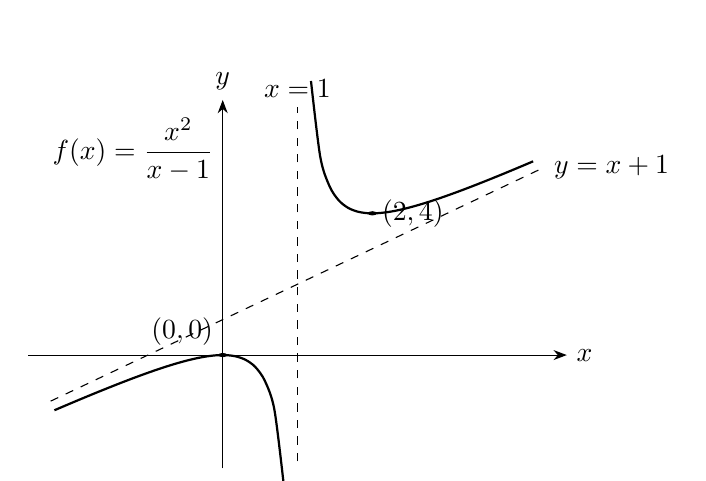
\begin{tikzpicture}[xscale=0.95,yscale=0.45,>=Stealth]
  \draw[->] (-2.6,0)--(4.6,0) node[right] {$x$};
  \draw[->] (0,-3.2)--(0,7.2) node[above] {$y$};
  \draw[dashed] (1,-3.0)--(1,7.0) node[above] {$x=1$};
  \draw[dashed] (-2.3,-1.3)--(4.3,5.3) node[right] {$y=x+1$};
  \draw[domain=-2.25:0.82,smooth,variable=\x,thick]
    plot ({\x},{\x+1+1/(\x-1)});
  \draw[domain=1.18:4.15,smooth,variable=\x,thick]
    plot ({\x},{\x+1+1/(\x-1)});
  \fill (0,0) circle (1.7pt) node[above left] {$(0,0)$};
  \fill (2,4) circle (1.7pt) node[right] {$(2,4)$};
  \node at (-1.2,5.8) {$f(x)=\dfrac{x^2}{x-1}$};
\end{tikzpicture}
\end{center}


\subsection{凸性与机器学习优化}

凸性在优化问题中非常重要. 直观地说，凸函数的图像没有“局部低谷冒充全局最低点”的现象. 在一元情形下，若 $f''(x)\ge0$，则 $f$ 为下凸函数；若严格凸且存在临界点，那么该临界点就是全局最小点. 许多基础机器学习模型，例如线性回归的均方误差损失，关于参数是凸函数，因此可以用导数和梯度方法稳定地寻找最优参数.

\begin{example}
设单样本线性模型损失为
\[
L(w)=\frac12(wx-y)^2,
\]
其中 $x,y$ 为常数. 讨论 $L$ 关于 $w$ 的凸性.
\end{example}
\begin{solution}
对 $w$ 求导：
\[
L'(w)=x(wx-y),\qquad L''(w)=x^2\ge0.
\]
因此 $L$ 关于 $w$ 是下凸函数. 若 $x\neq0$，则 $L''(w)=x^2>0$，函数严格凸，唯一最小点由 $L'(w)=0$ 给出，即
\[
w=\frac{y}{x}.
\]
若 $x=0$，则 $L(w)=\frac12y^2$ 为常数函数，任意 $w$ 都是最小点.
\end{solution}

\subsection{Taylor 公式}

\begin{theorem}[Taylor 公式：Lagrange 余项]
若 $f$ 在含 $x_0$ 与 $x$ 的区间上有 $n+1$ 阶连续导数，则存在介于 $x_0$ 与 $x$ 之间的 $\xi$，使得
\[
f(x)=\sum_{k=0}^{n}\frac{f^{(k)}(x_0)}{k!}(x-x_0)^k
+\frac{f^{(n+1)}(\xi)}{(n+1)!}(x-x_0)^{n+1}.
\]
\end{theorem}
\begin{proofdetail}
记
\[
P_n(t)=\sum_{k=0}^{n}\frac{f^{(k)}(x_0)}{k!}(t-x_0)^k.
\]
固定 $x\neq x_0$，令
\[
R=f(x)-P_n(x),\qquad
M=\frac{R}{(x-x_0)^{n+1}}.
\]
构造
\[
F(t)=f(t)-P_n(t)-M(t-x_0)^{n+1}.
\]
由 $P_n$ 的构造可知
\[
F(x_0)=F'(x_0)=\cdots=F^{(n)}(x_0)=0,
\]
且由 $M$ 的定义，$F(x)=0$. 对 $F$ 在以 $x_0,x$ 为端点的区间反复使用 Rolle 定理：由 $F(x_0)=F(x)=0$，存在一点使 $F'=0$；又 $F'(x_0)=0$，可在相应子区间再次使用 Rolle 定理，逐次得到存在 $\xi$ 介于 $x_0$ 与 $x$ 之间，使
\[
F^{(n+1)}(\xi)=0.
\]
而
\[
F^{(n+1)}(t)=f^{(n+1)}(t)-M(n+1)!.
\]
故
\[
M=\frac{f^{(n+1)}(\xi)}{(n+1)!}.
\]
代回 $R=M(x-x_0)^{n+1}$，得 Taylor 公式.
\end{proofdetail}

\begin{example}[Maclaurin 公式]
写出 $\ee^x,\sin x,\ln(1+x)$ 在 $0$ 处到常用阶数的展开.
\end{example}
\begin{solution}
\[
\ee^x=1+x+\frac{x^2}{2!}+\cdots+\frac{x^n}{n!}+o(x^n).
\]
\[
\sin x=x-\frac{x^3}{3!}+\frac{x^5}{5!}+\cdots+(-1)^m\frac{x^{2m+1}}{(2m+1)!}+o(x^{2m+1}).
\]
\[
\ln(1+x)=x-\frac{x^2}{2}+\frac{x^3}{3}-\cdots+(-1)^{n-1}\frac{x^n}{n}+o(x^n).
\]
这些公式可由 Taylor 公式和各阶导数在 $0$ 处的值推出.
\end{solution}

\begin{example}[极限]
求 $\displaystyle\lim_{x\to0}\frac{\cos x-1+\frac{x^2}{2}}{x^4}$.
\end{example}
\begin{solution}
由 Taylor 展开
\[
\cos x=1-\frac{x^2}{2}+\frac{x^4}{24}+o(x^4).
\]
故分子为
\[
\left(1-\frac{x^2}{2}+\frac{x^4}{24}+o(x^4)\right)-1+\frac{x^2}{2}
=\frac{x^4}{24}+o(x^4).
\]
因此极限为 $1/24$.
\end{solution}

\begin{example}[用 Taylor 判别极值]
设 $f'(x_0)=f''(x_0)=0$，$f^{(3)}(x_0)\neq0$. 证明 $x_0$ 不是极值点.
\end{example}
\begin{solution}
由 Taylor 公式，
\[
f(x)=f(x_0)+\frac{f^{(3)}(x_0)}{3!}(x-x_0)^3+o((x-x_0)^3).
\]
记 $A=f^{(3)}(x_0)/6\neq0$. 则
\[
f(x)-f(x_0)=(x-x_0)^3[A+o(1)].
\]
当 $x$ 足够接近 $x_0$ 时，$A+o(1)$ 与 $A$ 同号. 而 $(x-x_0)^3$ 在 $x_0$ 两侧异号，所以 $f(x)-f(x_0)$ 在两侧异号. 因此 $f(x_0)$ 既不是局部极大值，也不是局部极小值.
\end{solution}

\subsection{课后习题（二）：凸性、渐近线与 Taylor 公式}
\begin{enumerate}[label=\textbf{练习\arabic*.},leftmargin=2.2em]
\item 讨论 $y=x^4-2x^2$ 的凸性与拐点.
\item 求 $f(x)=\frac{x^2+1}{x-1}$ 的垂直渐近线与斜渐近线.
\item 用 Taylor 公式求下列极限或近似：
\[
\lim_{x\to0}\frac{\ln(1+x)-x+\frac{x^2}{2}}{x^3},\quad
\lim_{x\to0}\frac{\ee^{x^2}-1}{1-\cos x},\quad
\sqrt[3]{8.12}.
\]
\end{enumerate}

\subsection{参考解答（二）}
\begin{enumerate}[label=\textbf{练习\arabic*.},leftmargin=2.2em]
\item
\[
y''=12x^2-4=4(3x^2-1).
\]
当 $|x|<1/\sqrt3$ 时 $y''<0$，曲线上凸；当 $|x|>1/\sqrt3$ 时 $y''>0$，曲线下凸. 拐点为
\[
\left(\pm\frac1{\sqrt3},\,\frac19-\frac23\right)=\left(\pm\frac1{\sqrt3},-\frac59\right).
\]
\item $x=1$ 是垂直渐近线. 作除法：
\[
\frac{x^2+1}{x-1}=x+1+\frac2{x-1},
\]
故斜渐近线为 $y=x+1$.
\item
\[
\ln(1+x)=x-\frac{x^2}{2}+\frac{x^3}{3}+o(x^3),
\]
故第一个极限为 $\frac13$. 又
\[
\ee^{x^2}-1=x^2+o(x^2),\qquad 1-\cos x=\frac{x^2}{2}+o(x^2),
\]
第二个极限为 $2$. 对 $\sqrt[3]{8.12}$，取 $f(x)=x^{1/3}$，在 $x=8$ 处线性化：
\[
\sqrt[3]{8.12}\approx2+\frac{1}{3\cdot 8^{2/3}}\cdot0.12=2+\frac{0.12}{12}=2.01.
\]
\end{enumerate}

\clearpage
\renewcommand{\refname}{References}
\addcontentsline{toc}{section}{References}
\begin{thebibliography}{99}
\bibitem{JJ} 龚德恩. 经济数学基础：第一分册，微积分. 四川人民出版社. 2016.
\bibitem{TJ} 同济大学数学系. 高等数学. 高等教育出版社.
\bibitem{CJX} 陈纪修，於崇华，金路. 数学分析. 高等教育出版社.
\bibitem{Stewart} Stewart, J. \emph{Calculus: Early Transcendentals}. Cengage Learning.
\bibitem{MacTutorGreek} MacTutor History of Mathematics Archive. Euclid, Archimedes, Apollonius biographies. \url{https://mathshistory.st-andrews.ac.uk/}
\bibitem{MacTutorChinese} MacTutor History of Mathematics Archive. Chinese mathematics overview. \url{https://mathshistory.st-andrews.ac.uk/HistTopics/Chinese_overview/}
\bibitem{MacTutorCalculus} MacTutor History of Mathematics Archive. The rise of calculus. \url{https://mathshistory.st-andrews.ac.uk/HistTopics/The_rise_of_calculus/}
\bibitem{SEP-AI} Stanford Encyclopedia of Philosophy. Artificial Intelligence. \url{https://plato.stanford.edu/entries/artificial-intelligence/}
\bibitem{MathWorldFib} Wolfram MathWorld. Fibonacci Number. \url{https://mathworld.wolfram.com/FibonacciNumber.html}
\end{thebibliography}

\end{document}
